\documentclass{jcgt}
\usepackage{amsthm}
\usepackage{cleveref}
\newtheorem{definition}{Definition}
\setciteauthor{Alexander Sannikov}
\setcitetitle{Radiance Cascades}
%\setheadtitle{Abbreviated title, only if full title won't fit in page headers}

% Mark submissions with the date of submission using the following line:
\submitted{\today}

% Once an article is accepted accepted, switch to the following line and comment the preceding one. The editor will supply the argument values.
\accepted{submitted}{accepted}{published}{Editor Name}{vol}{issue}{1}{1}{year}
\seturl{http://jcgt.org/published/vol/issue/num/}


%%%%%%%%%%%%%%%%%%%%%%%%%%%%%%%%%%%%%%%%%%%%%%%%%


\begin{document}

\title{Radiance Cascades:\\A Novel Approach to Calculating Global Illumination[WIP]}

\author
       {Alexander Sannikov\\Grinding Gear Games
       }

\teaser{
  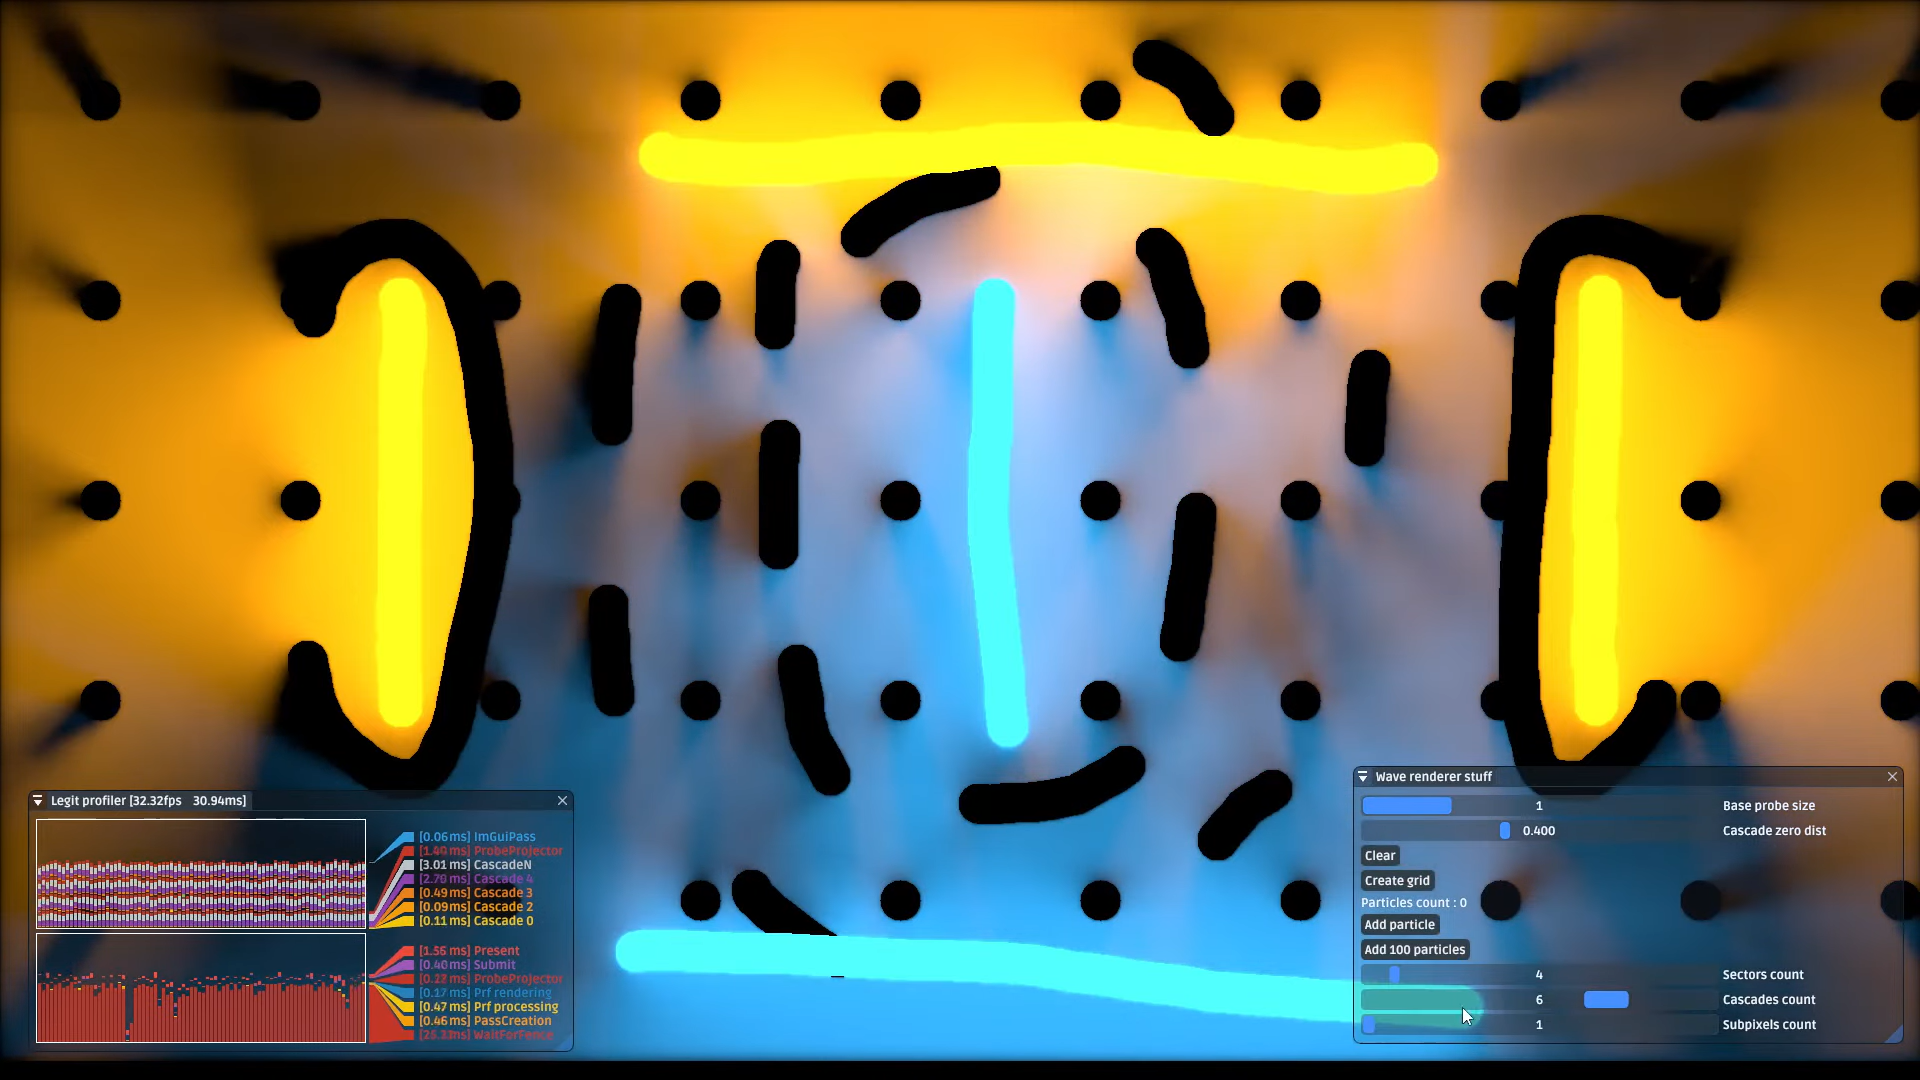
\includegraphics[width=0.9\textwidth]{images/gi_2d.png}
  \caption{\emph{Radiance cascades} used to calculate single-shot dynamic per-pixel global illumination in 2d.}
  \label{fig:teaser}
}

\maketitle
\thispagestyle{firstpagestyle}

\begin{abstract}
\small
This work proposes a novel data structure called \emph{radiance cascades} that allows effectively storing and calculating radiance field by decomposing it into multiple ranges (from near-field to far-field) and storing them separately. The idea of radiance cascades relies on an observation, that in order to resolve
radiance emitted by an object, one needs to have higher linear resolution next to it, and higher angular resolution farther away from it. \emph{Radiance cascades} exhibit a distinctly unique way of asymptotic scaling that for all practical purposes is equivalent to casting infinitely many rays in a finite amount of time, while using a finite amount of memory. This highly unusual property allows to effectively remove the total number of rays as the primary constraint for calculating global illumination in 2d and 3d.
\end{abstract}


%-------------------------------------------------------------------------
\section{Introduction}
\label{sec:introduction}
Global Illumination refers to the process of calculating more than one light bounce in rendering. This process is governed by the rendering equation:
\begin{equation}
  L_\mathrm{out}(\textbf{p}, \hat \omega_\mathrm{out}) = L_\mathrm{emi}(\textbf{p}, \hat \omega_\mathrm{out}) + \int_{\mathbb{S}^2} L_\mathrm{in}(\textbf{p}, \hat \omega_\mathrm{in}) \cdot f(\textbf p, \hat \omega_\mathrm{in}, \hat{\omega}_\mathrm{out}) \cdot |\hat{n} \cdot \hat{\omega}_\mathrm{in} |~ d\hat{\omega}_\mathrm{in}
  \label{eqn:rendering}
\end{equation}
  
This equation is notoriously hard to solve in the general case, either analytically or numerically, due to its inherent nature where every point of every object can cast or receive light from every other point of every other object and this light can also be occluded by any object between them. that is why in the field of graphics programming, the task of efficient calculation of global illumination has been one of the most crucial, yet among the most difficult tasks. In fact, some consider finding a fast and accurate solution to global illumination to be the ultimate goal or a holy grail of rendering.

Even though it is relatively straightforward to find an approximate solution to the rendering equation with methods like path tracing, these methods are generally not realtime \footnote{Notable "exception" of 1spp path tracing will be discussed in greater detail in \ref{sec:relatedwork}}, and even those methods that claim to be realtime in fact are typically not capable of converging to an accurate enough solution in one frame. This leads to a noisy solution and in order to mitigate it, practically all such methods have to heavily rely on spatial and/or temporal reuse of samples that inevitably leads to slow response of indirect lighting to scene changes and/or loss of high frequency details in indirect lighting.

As typically done in other approaches to solving global illumination, this work focuses primarily on calculating a single indirect bounce (including indirect light from emissive surfaces). The governing equation for this process can be represented with a non-recursive form of the rendering equation where the term $L_\mathrm{in}()$ is replaced with the part of lighting that can be calculated directly $L_\mathrm{direct}()$ with algorithms such as shadow mapping and using analytic light sources:
\begin{equation}
  L_\mathrm{out}(\textbf{p}, \hat \omega_\mathrm{out}) = L_\mathrm{emi}(\textbf{p}, \hat \omega_\mathrm{out}) + \int_{\mathbb{S}^2} L_\mathrm{direct}(\textbf{p}, \hat \omega_\mathrm{in}) \cdot f(\textbf p, \hat \omega_\mathrm{in}, \hat{\omega}_\mathrm{out}) \cdot |\hat{n} \cdot \hat{\omega}_\mathrm{in} |~ d\hat{\omega}_\mathrm{in}
  \label{eqn:reduced_rendering}
\end{equation}
This has become a standard practice in realtime rendering, because using an approach called \emph{radiosity}, this equation can be applied repeatedly to calculate multiple light bounces, and such a process converges to the same result as \ref{eqn:rendering}.

The main contribution of this work is proposing a novel data structure called radiance cascades that decomposes a radiance field into multiple ranges (from near-field to far-field) and stores each range in its own cascade. This way of representing radiance fields is quite memory-efficient and provides a natural way of calculating global illumination that is fast enough for many realtime applications and accurate enough to capture all frequencies of details: from high spatial frequency contact shadows to high angular frequency environment light.
In fact, radiance fields are built "from scratch" every frame without reusing any data from the previous frame, and in a matter of milliseconds allow calculating a solution to global illumination that is accurate enough so that it does not need any additional denoising. Another crucial property of radiance cascades is that they are completely geometry-agnostic: they encode radiance
at a constant cost that is independent of scene complexity, number of light sources or polygons present in the scene.

Each isolated radiance cascade is quite similar in its nature to a uniform grid of radiance probes, except instead of encoding full radiance, its probes store a different value called \emph{radiance interval} that corresponds to a specific range of the radiance field and a hierarchy of such cascades allows to accurately reconstruct the original radiance field.

Practical implementation of radiance cascades is integrated into Path of Exile 2 as its global illumination solution \Cref{fig:poe2gi}. That specific implementation uses a flatland-like screenspace radiance cascade hierarchy and populates them using screenspace raymarching -- a choice motivated by PoE2's fixed camera.

\begin{figure}[htb]
  \centering
  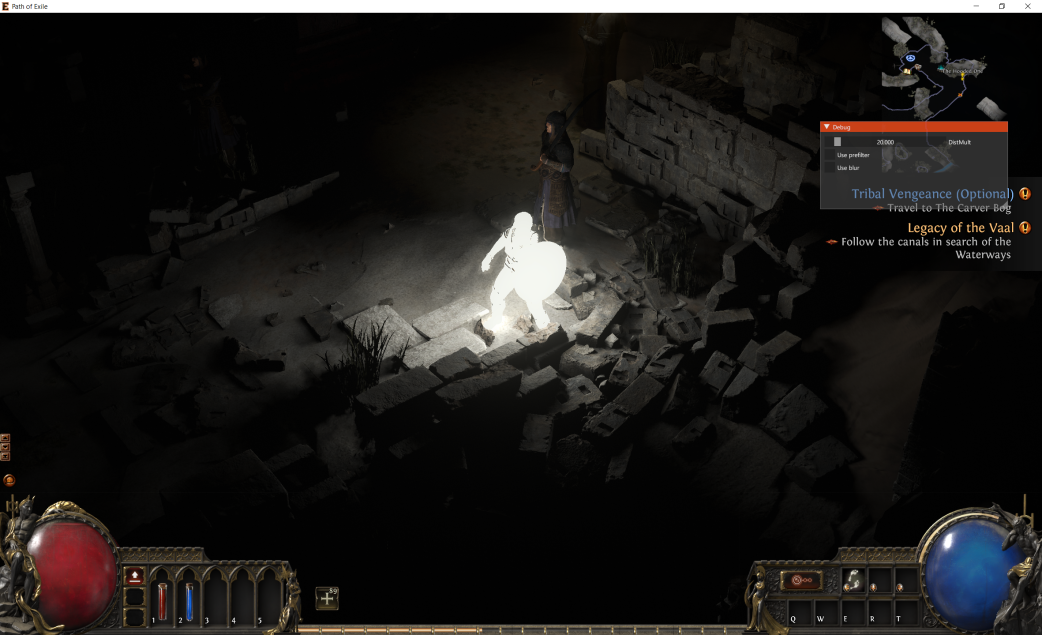
\includegraphics[width=0.49\columnwidth]{images/ranger_gi.png}
  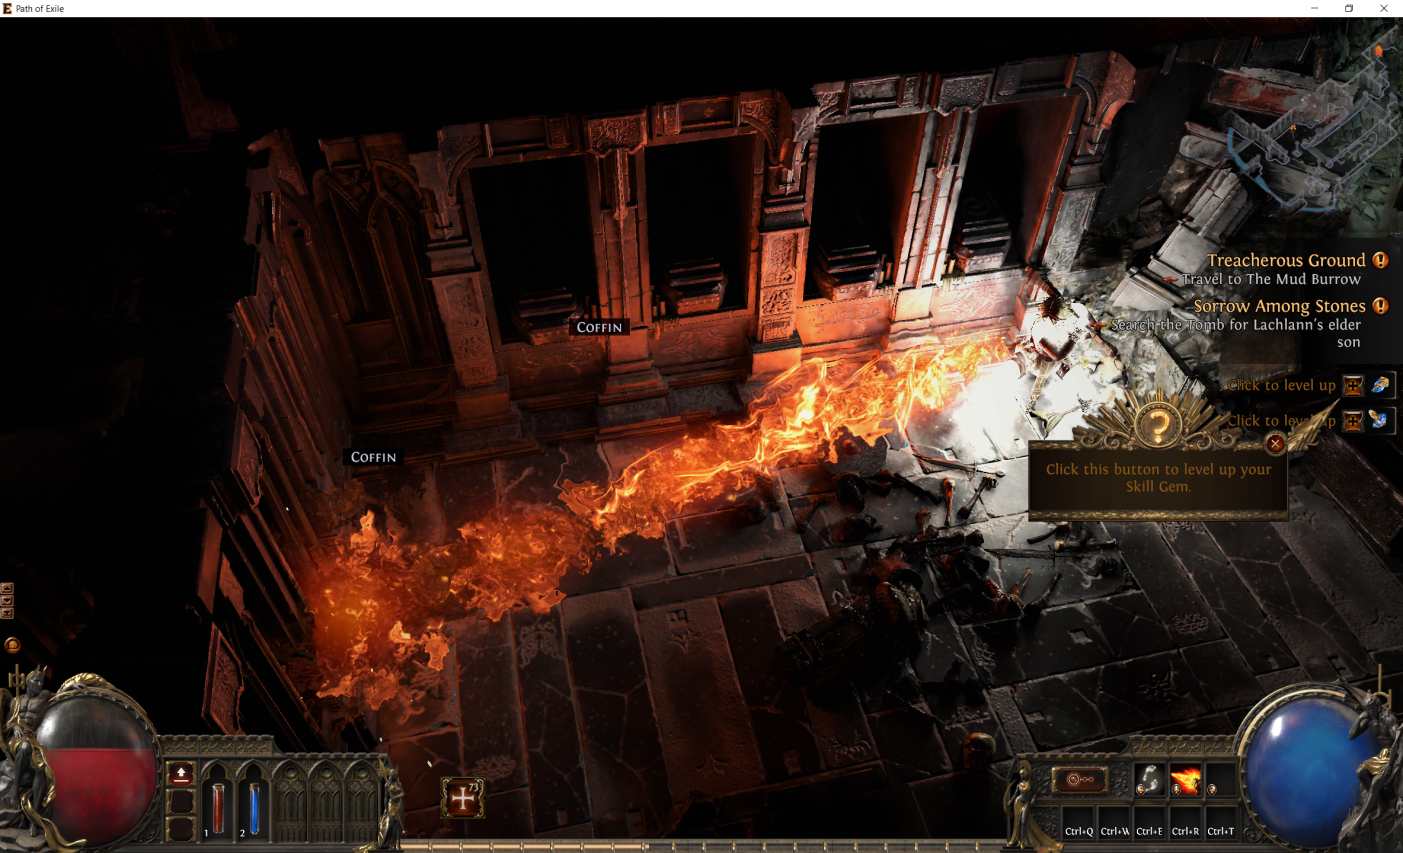
\includegraphics[width=0.49\columnwidth]{images/gi_with_specular.png}
  \caption{\label{fig:poe2gi}
     Left: PoE2 scene lit exclusively by indirect lighting emitted by a glowing character. Right: scene lit by indirect light created by a glowing character along with an emissive spell effect, includes both diffuse and specular components of indirect light.}
\end{figure}

In addition to calculating global illumination, \emph{radiance cascades} can also be directly observed, which can be useful for tasks such as rendering glossy reflections. Finally, radiance fields can be precalculated offline
capturing all view-dependent radiance data along with all material properties and all scene geometry and then rendered directly in near-constant time.


\subsection{Related Work and Motivation}
\label{sec:relatedwork}

The sheer number of approaches designed over the past 30+ years to find approximate solutions, under special conditions, to the problem of global illumination highlights how difficult this task truly is. The beauty and diversity of ideas behind some of these methods is truly inspirational and in one way or another has motivated this work.Unfortunately, many of these approaches, despite having amazing properties, see limited use in practice.

One example of a dramatically underused technique is \emph{imperfect shadow maps} or \emph{ISM} that allow practical encoding of surface radiance fields using atlases of
parabolically projected shadow maps created with rasterized point clouds assisted by postprocess gap filling. Truly inspirational technique that allows calculating global illumination with occlusion on old generation hardware at interactive framerates. Unfortunately, \emph{ISM} was never widely adopted, however, due to flaws in its scaling to large scenes.

An example of a completely different way of approaching the same problem would be \emph{light propagation volumes} also known as \emph{LPV}. \emph{LPV} encode radiance on a regular grid of probes that encode directional distribution with spherical harmonics and calculate radiance by solving continuous light propagation equations -- another beautiful idea, that enjoyed a relatively widespread adoption despite its fundamental limitations associated with light leaks and difficulties representing high frequency details.

A widely adopted idea is \emph{radiance probes} -- a fundamental data structure that captures incoming radiance into cubemap-like probes. While
being a very natural idea, the exact details of its implementation produce inevitable problems with light leaks and the exact way of calculating a large number of cubemaps especially for dynamic scenes is not exactly clear. A particularly curious decision that needs to be made before using \emph{radiance probes} is the tradeoff of how many radiance probes to use vs
what resolution to assign to each radiance probe. It is interesting to note that every implementation of \emph{radiance probes} seems to arbitrarily decide its position on this spectrum of the linear vs angular resolution tradeoff, and the search for the optimal answer to this conundrum has been one of the major motivations for this work. Another curious observation about grids of radiance probes are the eternal problems associated with their light leaking through walls and especially slopes at an angle: while it has been entertaining to see every game development studio come up with its own set tools to somewhat mitigate this problem, the problem is clearly fundamental to the idea of trying to discretize radiance on a regular grid. This search served as yet another inspiration for this work and prompted partitioning radiance fields into individual components (further referred to as \emph{radiance intervals}) that can be interpolated without introducing light leaks.

Seemingly unrelated at first glance, ubiquitous techniques such as \emph{environment mapping} and \emph{ambient occlusion} can actually be considered as approximations to the global radiance field and
naturally approximate the solution to global illumination. More specifically, environment mapping is an approximation far-field radiance directional distribution that captures no spatial information, while ambient occlusion captures specially localized occlusion with no directional information. And it is widely known how well these two extremes compliment each other: typically near-field ambient occlusion attenuating far-field environment light is present in practically every modern realtime renderer. However,a natural question to ask here is whether it is possible to define more intermediate steps between these two extremes of near-field and far-field. Is it possible to create more mid-field representations of the global radiance field that can synergize with each other as well as environment mapping synergizes with ambient occlusion? Well, the answer is yes and radiance cascades do exactly that.

A whole family of related work stems from approaches that precalculate and cache radiance and/or irradiance, effectively precalculating global illumination.
One such approach is light maps -- unfortunately, despite being widely adopted, it provides no easy way of storing the directional aspect of precomputed radiance. Attempts to store directional information in texture space have evolved to approaches such as precomputed radiance transfer. Despite being practically useful due to their precomputed nature, these methods have always been quite limited due to their precomputed nature. While radiance cascades proposed in this work can be also used for storing static precalculated radiance, they also offer an efficient way of calculating it fully dynamically.

Another relatively popular approach to calculating global illumination is voxel cone tracing. VCT approximates average radiance coming from a cone by a series of averaged boxes of increased size along its main axis. This can be done relatively cheaply by voxelizing the scene, building volumetric mipmaps and then by marching along a ray while also sampling higher and higher mip levels. Voxel cone tracing enjoyed some adoption in the industry but unfortunately suffered from significant problems associated with scaling to scenes of large volumes.
However, its core idea of averaging outgoing radiance from multiple points by building mipmaps was very fruitful and was later used in my original Path of Exile global illumination solution.


Among most recently developed practically useful global illumination solutions are hybrid approaches such as Lumen and GI-1.0. Despite being commercially successful, these methods have to rely quite a lot on spatiotemporal filtering, effectively
losing high frequency occlusion and creating ghosting artifacts. These hugely inspirational methods have brought the industry slightly closer to solving the problem of global illumination once and for all, but their spatiotemporal filtering artifacts as well as problems calculating far-field indirect light from small light sources are still open problems. These methods store radiance in two hierarchy levels: one level of screenspace radiance probes and a higher level of a worldspace radiance cache. One might say that they also have two more levels of
this emerging hierarchy: good old ambient occlusion and environment mapping. This fact more than ever begs the same questions: Why are there only 4 levels now? How many levels can there be? How many levels is
it reasonable to have? Is it possible to have a uniform representation for all such levels? Again, these questions ultimately lead to the idea of radiance cascades.

Problems associated with artifacts due to spatiotemporal filtering are far from being unique to Lumen and GI-1.0. In fact, it seems that there's a prominent trend in the industry right now towards having more sparse approximation of the radiance function while putting more work towards "fixing" it with spatiotemporal denoisers. In fact,
the extreme case of 1 sample per pixel path tracing with RESTIR and AI spatiotemporal denoisers seems to gain more and more popularity due to simplicity of the main idea behind it. The main idea behind these can be formulated as a practical decoupling of the problem of creating an accurate (albeit very coarse) discretization of the radiance field with path tracing and then
solving the problem of "filling the gaps" in such approximations with increasingly complex methods. Even though this approach can look very tempting, my strong belief is that the fundamental idea of reconstructing full radiance field from its crude approximation is inherently flawed. In other words, the core idea of reusing rays between spatially and temporally
adjacent rays is flawed: rays can be spatially incoherent for example on shadow boundaries and temporally incoherent in dynamic scenes. that is also the primary failure modes of all such methods: sharp contact shadows and highly dynamic scenes. A strategy much more efficient than reusing spatially adjacent radiance samples is reusing \emph{radiance intervals} (a property defined later on in this paper). And if done properly, that in itself is sufficient to not even rely on temporal coherence: just sharing radiance intervals between as many points as possible
is already sufficient to find an accurate enough solution to the problem of global illumination in realtime. And the answer is yet again, radiance cascades: the data structure designed with the goal of
sharing radiance intervals among as many points as possible. That being said, the accuracy of radiance cascades can be further dramatically increased if one does want to make use of temporal coherence,
although every application of radiance fields in this paper explicitly does not rely on temporal reuse and reacts instantaneously to arbitrarily dramatic scene, viewport and lighting changes.

Due to the considerations above, my personal belief is that even when hardware will at last become powerful enough to indeed solve global illumination with path tracing in real time, nobody will actually do so, just like nobody sorts arrays with bubble sort today, despite modern hardware is already powerful enough to sort most arrays in realtime with bubble sort. Bubble sort is still out of fashion just because strictly better sorting methods were discovered. 
Methods of calculating global illumination will keep getting better, and this includes unbiased solvers. As hardware becomes more powerful, much more efficient methods will be available and it will be simply more efficient to use them most of the time.

Last but not least, one global illumination solution that I find quite promising is my previous algorithm that is been shipped with Path of Exile since 2018 that I first implemented in 2017, which will be later referred to as \emph{hierarchal screenspace variance-based global illumination}, or \emph{HSSVGI}.
HSSVGI was roughly based on the idea of approximating radiance with horizon-based screenspace sectors, while each sector is calculated using screenspace mipmaps, and occlusion within a sector was approximated by a VSM-like Chebyshev inequality that utilizes the first two linear depth moments.
I have never published a paper on that one, but I explained it in my Exilecon 2019 presentation, and surprisingly in 2018 completely independently from me another author published a paper called
"Horizon-Based Indirect Lighting (HBIL)" by Benoît “Patapom” Mayaux that described a very similar approach.

However, even though \emph{HSSVGI} clearly had a lot of extremely valuable properties (in fact, they were valuable enough for it to become the first algorithm of its kind to be shipped
with a released game, Path of Exile), I knew from the beginning that there still were crucially important properties of radiance fields that it did not exploit. Namely, it had a denoiser stage that effectively shared irradiance between spatially adjacent points to reduce the noise. However, as was mentioned earlier, the core idea of sharing radiance produces an inevitable tradeoff between high frequency details of indirect light and the quality of denoising. And a proof to the fact that this could be done much better was also my algorithm for
calculating hierarchical screenspace shadow cascades that was implemented a couple years prior to that and explained as well during the 2019 Exilecon presentation. Its core idea was to calculate
blurrier parts of shadow penumbras \footnote{Arguably, the plural form of "penumbra" should be "penumbrae", but alas.} in lower resolution render targets/cascades and sharper contact shadows in higher resolution render targets, and then to effectively combine them. This
approach to rendering shadows by its very construction was exceptionally successful at representing penumbras, where blurry parts of penumbras were achieved for free just from the way these shadows were
stored in memory instead of the typical way achieved by blurring hard shadows. In fact, blurrier parts of penumbras are cheaper to calculate in such an approach compared hard shadows, which is a uniquely valuable property to have. The success of that algorithm kept fuelling my search for a way to construct a global illumination algorithm that would have the same property of capturing both
hard contact shadows as well as far-field blurry shadows. Again, finally realizing this idea in radiance cascades.



\section{Derivation}
To calculate global illumination efficiently, it's worth exploring geometric properties of radiance fields. Even though the radiance function $L(\textbf p, \hat \omega)$ on the first glance might look like a general-case 5d function ($\textbf p \in \mathbb{R}^3, \hat \omega \in \mathbb{S}^2$), it actually has internal constraints that can be exploited to represent it much more efficiently than that.

%\subsection{Disclaimer from the author}
%By writing this paper I deliberately put myself into an academically vulnerable position due to a certain level of slack that I allow myself in mathematical formalisms that follow, and occasional downright abuse of mathematical notation. Even though this does bring me great shame, it is not done with a malicious intent of hiding sneakily attached strings. This is done because I pursue no academic goals with this publication, and most explicitly there's no goal for me to provide a bulletproof mathematically rigorous foundation to my ideas. No. Instead, my only goal is to as clearly as possible relay the ideas behind \emph{radiance cascades} as well as the thought process that led to their creation and a way of justifying my choice of their parameters. This means that if an apt reader notices a clear flaw in my formal notation, but understands my intent behind it, I will consider my mission to be accomplished successfully.

\subsection{The Penumbra Condition}
The idea of radiance cascades relies on a crucial observation, that in order to resolve radiance emitted by an object of a given size, one needs to have higher linear resolution with lower angular resolution near this object, and lower linear resolution with higher angular resolution farther away from it.

One way to arrive at a formal definition of such a property is to explore the geometric structure of penumbras and the necessary conditions required to approximate penumbra's corresponding radiance field in a discrete fashion. Most notably, to accurately represent radiance of a penumbra, one needs to accurately capture both its sharp contact shadows in its near-field as well as its
wide blurred region in the far-field.

\begin{figure}[htb]
  \centering
  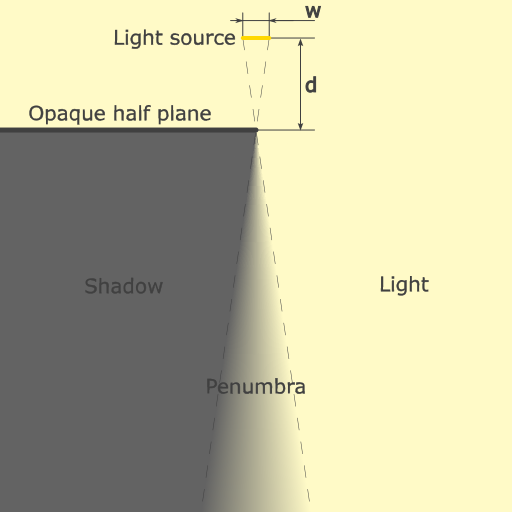
\includegraphics[width=0.5\columnwidth]{images/penumbra.png}
  \caption{\label{fig:penumbra} Penumbra occurs due to partial occlusion of an area light source.}
\end{figure}

To formally define such a condition, consider a penumbra produced by the smallest light source in the scene of linear size $w$ located at a small distance $d$ away from an infinite half plane (Figure \ref {fig:penumbra}).
Such a configuration produces a linear penumbra of angle
$
  \alpha = 2\arctan\left(\frac{ w}{2d}\right) \sim \frac{w}{d}
  \label{eq:pen_ang}
$. In order to resolve such penumbra at a given distance $D$ away from the light source\footnote{The condition of $D \gg d$ is actually not necessary, but it is easier to assume so in order to avoid defining $D + d$ as a distinct value and instead assume that $D+d \approx D$} ($D \gg d$),
one needs to have a linear discretization step of smaller than 
\begin{equation}
\Delta_p < \alpha D = 2\arctan\left(\frac{ w}{2d}\right) D
\label{eq:delta_p_big}
\end{equation}

\begin{figure}[htb]
  \centering
  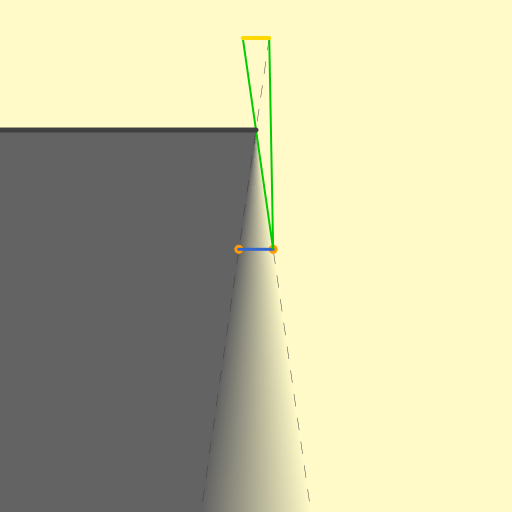
\includegraphics[width=0.49\columnwidth]{images/penumbra probes 1.png}
  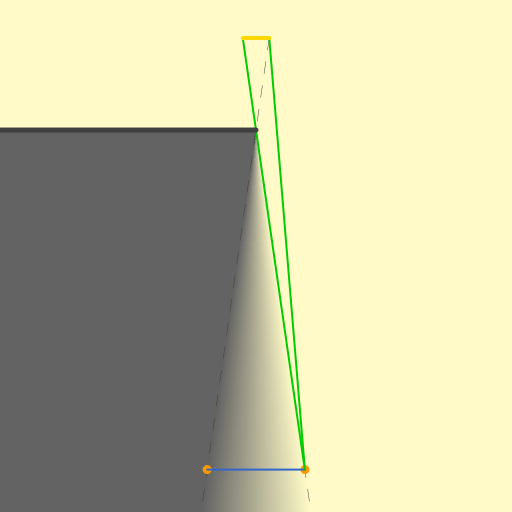
\includegraphics[width=0.49\columnwidth]{images/penumbra probes 2.png}
  \caption{\label{fig:penumbra2}
  Left: to properly resolve a penumbra, two probes (shown in orange) located close to its origin need comparatively small linear discretization steps (shown in blue) and comparatively large angular discretization steps (shown in green). Right: more distant radiance probes can have higher linear discretization steps, but require lower angular discretization in order to resolve the same penumbra.}
\end{figure}
since that is the linear width of such penumbra at distance D. However, since the penumbra is physically produced by partial occlusion of a light source, it is also necessary to have sufficient angular resolution to resolve the light source itself with enough detail to capture its partial occlusion, so the angular discretization step needs to be smaller than the angular size of the light source at distance $D$ which is equal to
\begin{equation}
  \Delta_\omega < w/D
  \label{eq:delta_w_big}
\end{equation}

To summarize, let's combine inequalities \ref{eq:delta_p_big} with \ref{eq:delta_w_big} to define the way the linear discretization step $\Delta_p$
as well as the angular discretization step $\Delta_w$ need to scale with distance $D$ from the light source, by fixing characteristic parameters of the scene $w$ and $d$ (Figure \ref {fig:penumbra2})\footnote{From now on, notation $A \sim B$ should be interpreted as "A scales linearly as a function of B" and $A <\sim B$ should be interpreted as "A is less than some function that scales linearly with B".} :

\begin{equation}
  \begin{cases}
    \Delta_p <\sim D, \\
    \Delta_\omega <\sim 1/D
  \end{cases}
  \label{eq:pen_cond}
\end{equation}

Let's call such relationship \emph{the penumbra condition} for the lack of a better term. To reiterate, this condition defines the way radiance discretization stepping needs to scale with distance in order to accurately encode penumbras.

\subsection{The Penumbra Hypothesis}

Let's define \emph{The Penumbra Hypothesis} as an assumption that for a given discretization of radiance field to be representative of the field at every scale, it is necessary and sufficient for such discretization
to satisfy the penumbra condition associated with such radiance field. \footnote{
Admittedly the exact meaning of what it means for a field discretization to be "representative" is at best nebulous (and more realistically, ambiguous), hopefully its exact meaning will become more apparent from the way it will be used in Section \ref{interpolateability}.}

A perfectly logical question to ask at this point is whether this hypothesis even holds in reality or not at all. Apparently, while there are certain edge cases when this assumption can be demonstrated to fail(namely infinitesimally
small light sources located infinitesimally close to occluders), it turns out this assumption holds quite well for almost all practical purposes. In particular, it is worth noting that
this assumption holds for two of the most extreme cases of radiance approximation: ambient-occlusion-like near-field representation that captures very high spatial frequency occlusion $\Delta_p \to 0$ without capturing any directionality $\Delta_\omega \to +\infty$, as well as environment-mapping-like far-field information stored in environment maps without any spatial localization so that $\Delta_p \to +\infty$
but with sufficient angular accuracy such that $\Delta_\omega \to 0$. However, later on it will be shown that it is also possible to construct a continuum of approximations (radiance cascades) that can encode
these two extremes as well as everything in-between them.

Another way to give intuitive justification as to why such hypothesis should indeed hold in reality is to consider what it means for a discretization of a radiance field to satisfy the penumbra condition: it means that
such discretization can describe well enough any penumbra of angular size larger than $w/d$ and produced by any light source larger than $w$. And since an arbitrary radiance field can be thought of
superposition of penumbras, and the given approximation is representative of each one of them, it is also fair to assume that it is representative of the radiance field overall.

\subsection{Radiance Interval}
Assuming the penumbra hypothesis holds, in order to exploit its properties, it is essential to separately represent near-field and far-field radiance fields since they have different
discretization frequency requirements. In order to do so, let's define a new property called radiance interval. Radiance interval $L_{a,b}(\textbf{p}, \hat \omega)$ is defined as incoming radiance at point $\textbf{p}$ from ray direction $\hat \omega$, originating from points farther away than $a$, but closer than $b$, in relation to $\textbf{p}$. In other words, only points on the ray
\begin{equation}
  \textbf{p} + t \hat \omega, t \in [a,b]
\end{equation}
contribute to such radiance. For visual difference between radiance and radiance interval refer to Figure \ref{fig:radiance_interval_probe}

\begin{figure}[htb]
  \centering
  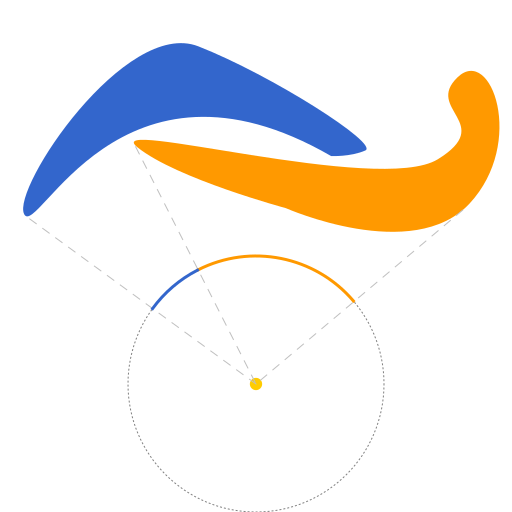
\includegraphics[width=0.49\columnwidth]{images/radiance probe.png}
  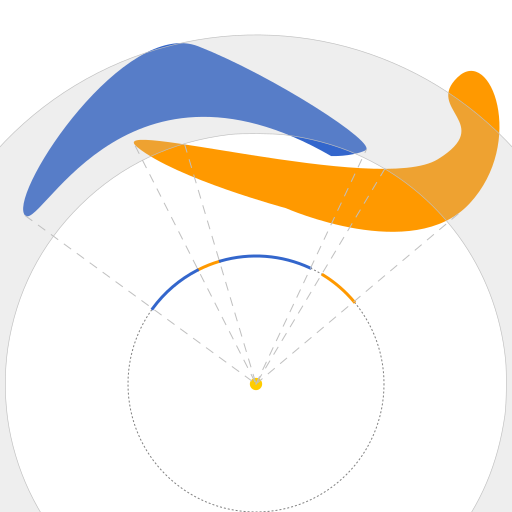
\includegraphics[width=0.49\columnwidth]{images/radiance interval probe.png}
  \caption{\label{fig:radiance_interval_probe}
  Left: radiance of two objects (orange, blue) encoded as angular distribution for a single radiance probe. Right: radiance interval corresponding to grayed out distance range encoded the same way.}
\end{figure}


 
In order to formally define \emph{radiance interval} in the opaque approximation (where each point of space is either completely transparent or completely opaque), one can use a raycasting function
$\textbf R(\textbf{p}, \hat \omega)$ that for a given point $\textbf{p}$ and direction $\hat \omega$ returns the nearest opaque surface in that direction. Using the raycasting function $\textbf R(\textbf{p}, \hat \omega)$ , we can formally define \emph{radiance interval} $L_{a,b}(\textbf{p}, \hat \omega)$ as:
\begin{equation}
  \label{eq:def_radiance_opaque}
  L_{a,b}(\textbf{p}, \hat \omega) = \left\{
    \begin{array}{ll}  
      L_{\mathrm{out}}(\textbf R(\textbf{p} + a\hat \omega, \hat \omega), -\hat \omega), & \text{if\ } |\textbf R(\textbf p + a \hat \omega, \hat \omega)-\textbf p| < b; \\
      0, & \text{otherwise}.
    \end{array}\right.
\end{equation}

It is also possible to define \emph{radiance interval} in the continuous case using volume rendering-like formulation for a continuous opacity distribution $\sigma(\textbf p)$:

\begin{equation}
  \label{eq:def_radiance_volume}
  L_{a,b}(\textbf{p}, \hat \omega) = 
  \int_a^b e^{-\int_a^x \sigma(\textbf p + y\hat \omega)dy} L_\mathrm{emi}(\textbf p+x\hat \omega, -\hat \omega)dx
\end{equation}

It is also useful to define in a similar fashion \emph{transparency interval}, that for a given point $\textbf{p}$, direction $\hat \omega$ and an interval $[a, b]$ returns transparency $\beta \in [0,1]$ of geometry on a ray segment $\textbf{p} + t \hat \omega, t \in [a,b]$. In other words, in the opaque approximation, transparency interval can be defined as
\begin{equation}
  \beta(\textbf p, \hat \omega)_{a, b} = \left\{
  \begin{array}{ll}  
    0, & \text{if\ } |\textbf R(\textbf p + a \hat \omega, \hat \omega)-\textbf p| < b; \\
    1, & \text{otherwise}.
  \end{array}\right.
\end{equation}
Or in continuous approximation:
\begin{equation}
  \beta(\textbf p, \hat \omega)_{a, b} =
  e^{-\int_a^x \sigma(\textbf p + y\hat \omega)dy}
\end{equation}
An intuitive understanding of radiance intervals can be acquired by looking at Figure \ref{fig:radiance_interval_probe} that demonstrates between classic radiance and a radiance interval, and also at Figure \ref{fig:3d_cascades} where radiance intervals of different ranges are displayed.
\begin{figure}[htb]
  \centering
  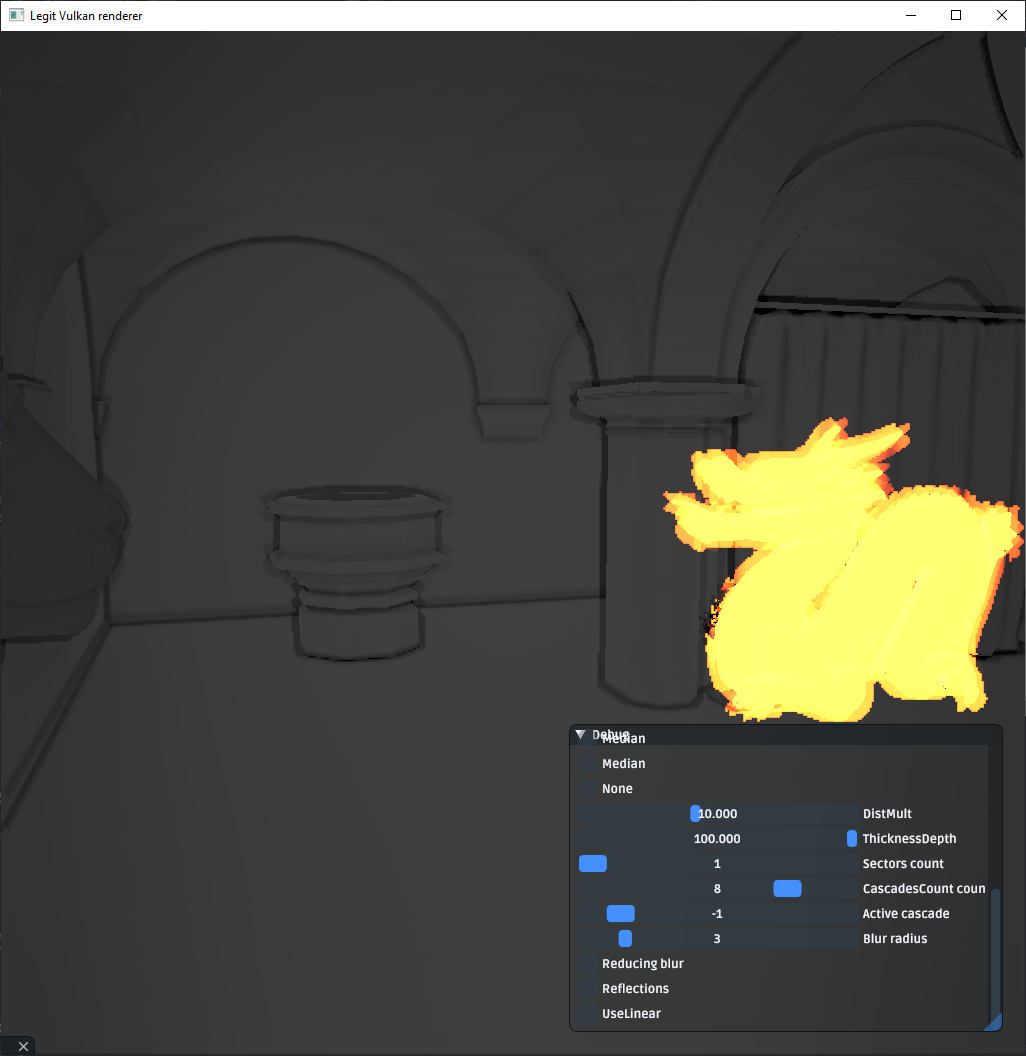
\includegraphics[width=0.32\columnwidth]{images/3d_cascade_0.png}
  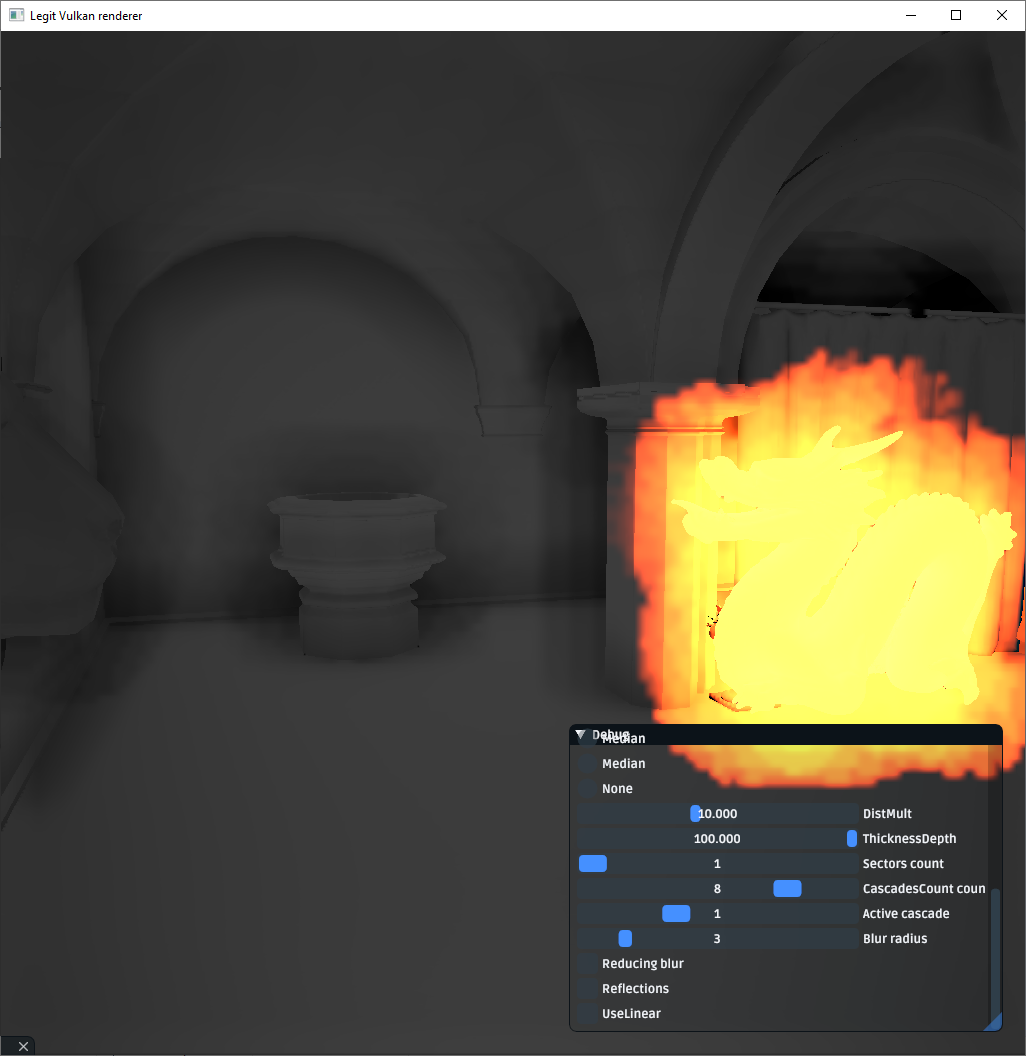
\includegraphics[width=0.32\columnwidth]{images/3d_cascade_2.png}
  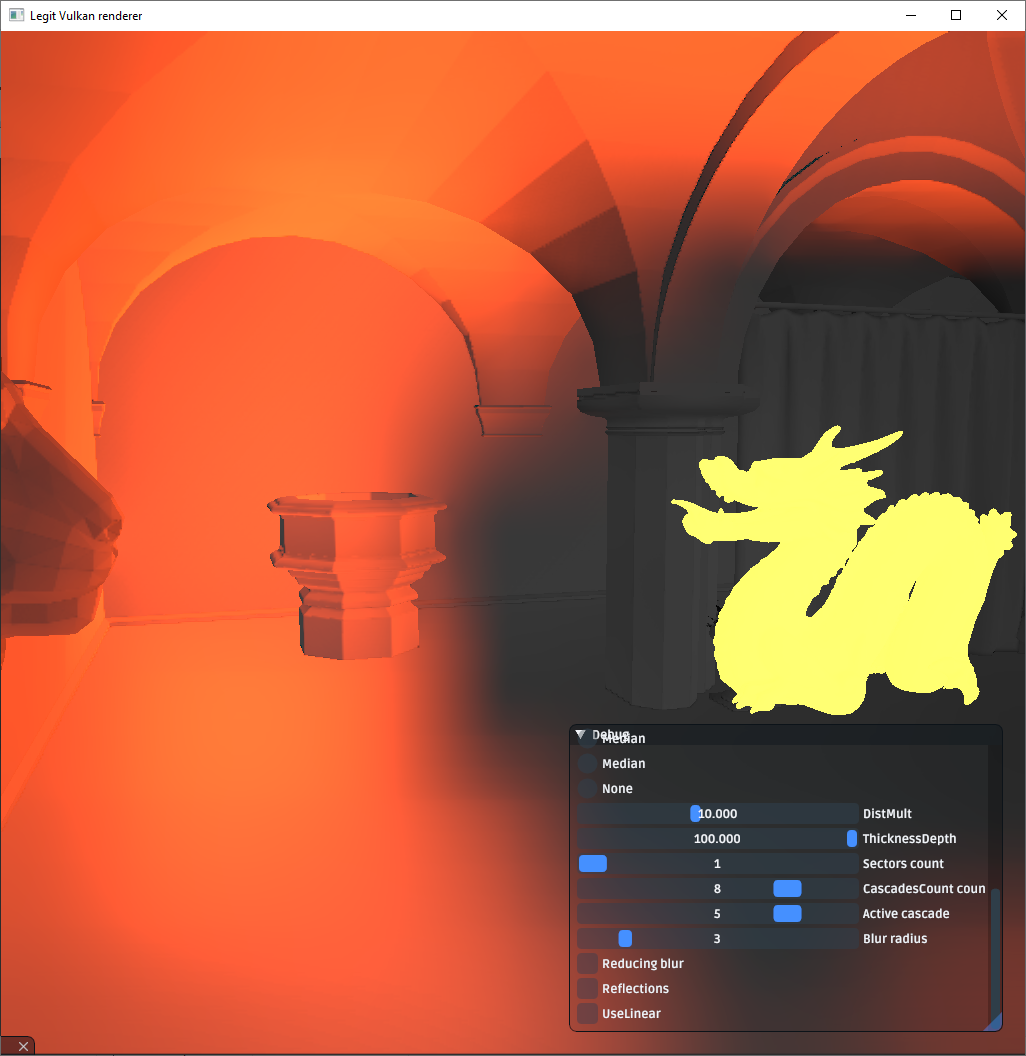
\includegraphics[width=0.32\columnwidth]{images/3d_cascade_5.png}
  \caption{\label{fig:3d_cascades}
     From left to right, cascades 0, 2, and 5 are shown. Note how each cascade captures a specific part of incoming radiance with a relatively consistent linear and angular frequency, hence allowing each cascade to be linearly interpolated.}
\end{figure}


\subsubsection{Merging radiance intervals}
A crucial observation should be made here that radiance intervals can be merged if their corresponding intervals are adjacent:
\begin{equation}
  \begin{cases}
    L_{a,c}(\textbf{p}, \hat \omega) = L_{a,b}(\textbf{p}, \hat \omega) + \beta(\textbf p, \hat \omega)_{a, b}L_{b,c}(\textbf{p}, \hat \omega)\\
    \beta(\textbf p, \hat \omega)_{a, c} = \beta(\textbf p, \hat \omega)_{a, b}\beta(\textbf p, \hat \omega)_{b, c}
    \label{eq:merging}
  \end{cases}
\end{equation}


The set of equations \ref{eq:merging} can be trivially derived from the formal definitions of \emph{radiance interval}. Intuitively, what this means is that when you look in a certain direction, what you see is simply what is located near you, on top of what is located away from you.

Next, let's notice that conventional radiance can be defined as radiance interval of an infinite half-interval:
\begin{equation}
  L_{\mathrm{in}}(\textbf{p}, \hat \omega) = L_{0,+\infty}(\textbf{p}, \hat \omega)
  \label{eq:infty_radiance}
\end{equation}
The intuitive meaning here is that when you look in any direction, what you see is the nearest of all things that are located anywhere from right next to you to infinitely far away.

And finally, by combining \ref{eq:merging} and \ref{eq:infty_radiance} it can be shown that radiance can be constructed by recursively "merging" N \emph{radiance intervals} $L_{t_i, t_{i+1}}(\textbf{p}, \hat \omega)$, if $t_0 = 0$ and $t_{N-1} = +\infty$:
\begin{equation}
  \begin{cases}
    L_{t_i,t_{i+2}}(\textbf{p}, \hat \omega) = L_{t_i,t_{i+1}}(\textbf{p}, \hat \omega) + \beta(\textbf p, \hat \omega)_{t_i, t_{i+1}}L_{t_{i+1},t_{i+2}}(\textbf{p}, \hat \omega)\\
    \beta_{t_i, t_{i+2}}(\textbf p, \hat \omega) = \beta_{t_i, t_{i+1}}(\textbf p, \hat \omega)\beta_{t_{i+1}, t_{i+2}}(\textbf p, \hat \omega)
    \label{eq:recursive_merging}
  \end{cases}
\end{equation}

Note that depending on the order of iterations, cascades can be merged either back-to-front as well as front-to-back, providing identical results, which is equivalent to classic back-to-front vs front-to-back blending or volume rendering.

\subsubsection{Shifting radiance intervals}
For a known radiance interval field
$L_{a,b}(\textbf{p}, \hat \omega)$
and some fixed direction $\hat \omega$, one can shift the range of such an interval by translating it in space along $\hat \omega$:
\begin{equation}
  \begin{cases}
    L_{a + x,b + x}(\textbf{p}, \hat \omega)=
      L_{a,b}(\textbf{p} + \hat \omega x, \hat \omega) \\
    \beta_{a + x,b + x}(\textbf{p}, \hat \omega)=
      \beta_{a,b}(\textbf{p} + \hat \omega x, \hat \omega)
  \end{cases}
  \label{eq:radiance_interval_shifting}
\end{equation}

The intuitive meaning is that points located on a ray segment $\textbf{p} + t \hat \omega, t \in [a+x,b+x]$ are the exact same point as points on a ray segment $\textbf{p} + x \hat \omega + t \hat \omega, t \in [a,b]$, because these are actually two ways to define the same segment.

This property can be derived in a more rigorous way by analyzing the definition of radiance interval \ref{eq:def_radiance_opaque} or  \ref{eq:def_radiance_volume}.


\subsubsection{Extending radiance intervals}
Another observation can be made by combining the equation for shifting radiance intervals \ref{eq:radiance_interval_shifting} with the equation for merging them \ref{eq:merging}. Namely, for a known radiance interval $L_{a,a+x}(\textbf{p}, \hat \omega)$, one can construct a shifted radiance interval: 
\begin{equation}
  \begin{cases}
    L_{a+x,a+2x}(\textbf{p}, \hat \omega)
      =L_{a,a+x}(\textbf{p}+x\hat \omega, \hat \omega) \\
    \beta_{a+x,a+2x}(\textbf{p}, \hat \omega)
      =\beta_{a,a+x}(\textbf{p}+x\hat \omega, \hat \omega)
  \end{cases}
\end{equation}
and this interval can be merged with the original $L_{a,a+x}(\textbf{p}, \hat \omega)$ to extend its range to $[a,a+2x]$, using the merging formulas \ref{eq:merging}:

\begin{equation}
  \begin{cases}
    L_{a,a+2x}(\textbf{p}, \hat \omega) = L_{a,a+x}(\textbf{p}, \hat \omega) + \beta(\textbf p, \hat \omega)_{a, a+x}L_{a,a+x}(\textbf{p} + x\hat \omega, \hat \omega)\\
    \beta_{a, a+2x}(\textbf p, \hat \omega) = \beta_{a, a+x}(\textbf p, \hat \omega)\beta_{a, a+x}(\textbf p+x\hat \omega, \hat \omega)
    \label{eq:extending_intervals}
  \end{cases}
\end{equation}
This means that methods utilizing raymarching don't need to actually raymarch an entire interval $[a, b]$ to calculate radiance $L_{a,b}(\textbf{p}, \hat \omega)$. Instead, it is possible to raymarch only the range $[a, a + \frac{b-a}{2}]$, store it in a radiance cascade and then extend this range twice by shifting and merging probes inside of the cascade in $O(1)$. Furthermore, even range $[a, a+\frac{b-a}{2}]$ can in turn be constructed by extending the range of $[a, a+\frac{b-a}{4}]$ just the same way. In other words, as long as precision allows, it is possible to avoid raymarching long paths and instead raymarch a tiny path and then keep iteratively doubling it by extending the cascade until it meets the necessary range.


%Another crucial observation here is that if \emph{the penumbra hypothesis} holds and \emph{radiance interval} $L_{a,b}(\textbf{p}, \hat \omega)$ is discretized by a set of points $(\textbf{p}_i, \hat \omega_i)$ that satisfies the penumbra condition, then the original function $L_{a,b}(\textbf{p}, \hat \omega)$ can be approximated well enough by linearly interpolating between discrete values $L_{a,b}(\textbf{p}_i, \hat \omega_i)$ \label{fact:int}. In fact, this property of linear interpolability(?) is what it in fact means for a discretization to be representative of a field in the definition of \emph{the penumbra hypothesis}.


\subsection{Radiance cascades}
\label{sec:radiance_cascades}
Now it is possible to construct a general-purpose scene-independent and BRDF-independent discretization scheme of an arbitrary radiance function $L(\textbf p, \hat \omega)$ that relies only on the penumbra hypothesis.
First, since the discretization needs to be scene-independent, we can't utilize any nonuniform sampling schemes such as importance sampling of BRDF, or explicit sampling of emissive surfaces and/or light sources.
Instead, we'll use only uniformly distributed samples in both space and direction. Second, we can encode radiance intervals corresponding to different ranges separately. In order to do so, let's define one radiance cascade as a linearly and directionally uniform discretization of radiance interval $[a, b]$ in accordance with the penumbra condition.
In order for such discretization to satisfy the penumbra condition, its linear and angular discretization steps must satisfy:
\begin{equation}
  \begin{cases}
    \Delta_p<\sim\min(a, b)=a \\
    \Delta_\omega<\sim \min(\frac{1}{a}, \frac{1}{b})=\frac{1}{b}
    \label{eq:interval_ranges}
  \end{cases}
\end{equation}
\label{interpolateability}
One crucially important property of radiance cascades is that if they satisfy the penumbra condition, then this representation is always linearly interpolateable. This holds because radiance cascades by construction encode data that has a maximum spatial frequency less than cascade's linear discretization frequency and angular frequency less than the cascade's directional discretization frequency, satisfying the Nyquist condition due to the way they are constructed. This means that the original radiance interval function can be reconstructed from its discrete samples without introducing distortion. In practice, this reconstruction can be done using linear interpolation between discrete radiance interval samples.

In fact, the way I originally came up with this data structure was by trying to find a way to discretize radiance in a way that is as sparse as possible, while minimizing the error associated with linear interpolation.

Just to re-iterate this once again: data stored in radiance cascades can be linearly interpolated in both space and direction, without the need of any bilateral filtering or disocclusion schemes frequently encountered in many techniques involving radiance probes. In fact, classic radiance probes indeed require special handling of disocclusion exactly \emph{because} they attempt to encode full radiance instead of encoding radiance intervals.

After defining one radiance cascade that encodes a given radiance interval, the next step is to define a sequence of such cascades that can be all combined together using \ref{eq:recursive_merging} to encode full radiance.
In order to achieve this, each cascade in such a sequence set needs to start exactly at the end of the cascade before it. In other words, cascade number $i$ encodes radiance interval $[t_i, t_{i+1}]$,
such that
\begin{equation}
  \begin{cases}
    t_{i+1}>t_i \\
    t_0 = 0 \\
    \lim_{i \to +\infty}t_i=+\infty
  \end{cases}
  \label{eq:ts}
\end{equation}

Now, let's decide what values of $t_i$ to choose, because anything that satisfies \ref{eq:ts} creates a valid sequence of cascades. However, not every choice of $t_i$ will produce cascades that can satisfy the penumbra condition while having sparse enough linear and angular stepping, since in practice it is beneficial to encode every cascade with as little information as possible, and the amount of required storage directly decreases with larger spatial and angular discretization stepping.

One natural way of producing a sequence of cascades that lends itself to efficient storage is by exponentially increasing probe linear stepping, so that probes of cascade $i+1$ are spaced apart twice as far away than probes of cascade $i$, similar to how mipmapping works, and then calculate their corresponding intervals $t_i$ and angular stepping $\Delta_\omega$ using the penumbra condition.

More specifically, the distance $\Delta_p$ between probes in the grid needs to increase exponentially $\Delta_p\sim2^i$, but also according to \ref{eq:interval_ranges}, $\Delta_p\sim t_i$, and combining them together leads to $t_i\sim2^i$.

Consequently, in order to satisfy \ref{eq:interval_ranges}, $\Delta_\omega$ must be defined as $\Delta_\omega\sim\frac{1}{t_{i+1}}=\frac{1}{2^{i+1}}\sim \frac{1}{2^i}$ (see Figure \ref{fig:cascades} for illustration). To sum up, in order to satisfy the penumbra condition, if every cascade has twice greater probe linear stepping than the previous cascade, it also needs to have twice smaller angular stepping and it needs to cover twice longer radiance interval:
\begin{equation}
  \begin{cases}
    \Delta_p\sim2^i \\
    \Delta_\omega\sim \frac{1}{2^i} \\
    t_i\sim2^i
  \end{cases}
  \label{eq:cascade_scaling}
\end{equation}


\subsection{Representing radiance cascades in memory}
  
Next step is deciding exactly how to encode each individual cascade $i$ in order to satisfy \ref{eq:cascade_scaling}, namely its necessary linear discretization step has to be $\Delta_p \sim 2^i$ and its angular discretization step has to be $\Delta_\omega\sim\frac{1}{2^i}$. A natural choice for this task is to use a data structure similar a regular grid of standard radiance probes (also known as light probes), where each probe is represented by its position in space and stores directional distribution of incoming radiance interval $L_{t_i, t_{i+1}}(\textbf p, \hat \omega)$ as rgb triplets + opacity $\beta_{t_i, t_{i+1}}(\textbf p, \hat \omega)$ in the alpha channel by means of storing them in a cubemap, octahedral map, spherical harmonics, etc. The exact representation of each radiance probe is not really relevant, what is relevant is how the amount of data that it needs to contain scales asymptotically, and all these representations scale exactly the same way. The only difference between a radiance cascade and typical radiance probes is that each radiance cascade stores a specific radiance interval, whereas radiance probes typically encode full radiance.


The amount of memory needed to store such cascades will crucially depend on the exact linear as well as angular dimensionality of the radiance field in question. 
For example, encoding full 3d radiance will obviously require storing more data compared to flatland.

Below are listed some examples of how to construct radiance cascades for typical cases of dimensionality used in rendering.


\subsubsection{Flatland}
\label{sub:flatland_scaling}
Radiance field of a flatland is defined as a 3d function (2d position + 1d direction/angle). One radiance cascade corresponding to radiance interval field of such dimensionality can be represented as a 2d grid of uniformly spaced radiance probes at linear distance $\sim2^i$ apart, and each probe needs to have $\sim\frac{1}{2^i}$ as its angular discretization step. This means that there 
needs to be a total of $P_i\sim \frac{1}{2^i}\cdot\frac{1}{2^i}$ probes, while each probe needs to store $Q_i=2^n$ angular "texels". This means that memory required to store such cascade is $M_i=P_iQ_i \sim \frac{1}{2^i}\cdot\frac{1}{2^i}\cdot 2^i = \frac{M_0}{2^i}$.

In other words, in flatland the memory required for discretizing radiance cascade $i$ scales as $M_i\sim\frac{1}{2^n}$. In other words, memory required to store cascade $i$ decreases exponentially as a function of $i$.

Now, memory required to store $N$ such cascades is simply the total memory required from each cascade added together, which is:
\begin{equation}
  \sum_{i=1}^{N}M_i\sim M_0/2^0+M_0/2^1+M_0/2^2+... = 2M_0
  \label{eq:constant_cost}
\end{equation}
In other words, the amount of memory required to store arbitrarily many radiance cascades in 2d is less than a constant, and it is exactly equal to twice the amount of memory required to store cascade 0. Figure \ref {fig:flatland_cascades} shows an example of what such layout can look like visually:
\begin{figure}[htb]
  \centering
  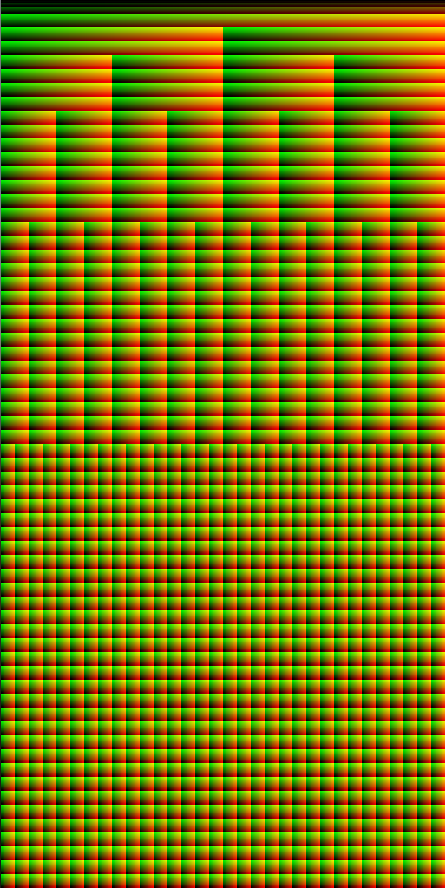
\includegraphics[height=\columnwidth, angle=-90]{images/flatland_cascades.png}
  \caption{\label{fig:flatland_cascades}
     An example of flatland radiance cascade hierarchy in memory: cascade 0 on the left has 32x32 probes, 8x8 angular texels each. Cascade 1 to the right from it has 16x16 probes, 8x16 texels each, etc. Width of this atlas is always equal to twice the width of cascade 0. }
\end{figure}

Note that even though flatland seems like a toy example of limited practical importance, it will be shown later that screenspace radiance of a 3d scene can be actually discretized in a way that scales the same way as how flatland \emph{radiance cascades} scale.


\subsubsection{3D space}
Radiance field of a regular 3d space is a function of 3d position $\textbf p(x, y, z)$ and a 2d direction $\hat \omega(\text{longitude}, \text{latitude})$, so $L(\textbf p, \hat \omega)$ is a 5d function. Once again, in accordance with \ref{eq:cascade_scaling} for cascade number $i$ and probes spaced apart at distance $\Delta_p\sim 2^i$ in a 3d regular grid, the total number of probes decreases as $P_i\sim(\frac{1}{2^i})^3$. Now, in order for each probe to have angular resolution 
$\Delta_\omega=\frac{1}{2^i}$, it needs to have an equivalent of $Q_i\sim(2^i)^2$ "cubemap texels". Cubemap texels here are taken in quotes because the exact representation of angular distribution is completely
irrelevant: it can be a cubemap, a parabolic projection map, octahedral mapping, spherical harmonics, the important property is that it is encoded with $Q_i\sim(2^i)^2$ floating point values. Now, total memory required to store cascade $i$ is $M_i=P_i*Q_i$ and can be expressed as $M_i\sim (\frac{1}{2^i})^3\cdot(2^i)^2=\frac{M_0}{2^i}$.

This means that even though the exact layout of each cascade in 3d is totally different compared with flatland, the total memory required to store cascade i decreases exponentially exactly the same way $1/2^i$. Because of this, infinitely many cascades add up to $\sum_{i=1}^{+\infty} M_i=2M_0$ in exactly the same way, which for a given size of $M_0$ is less than a constant.

\subsubsection{Surface radiance field in 3d}
\label{sub:surface_scaling}
Radiance of a 3d scene encoded on a 2d surface can be useful for applications such as baking surface lighting in 2d lightmaps and rendering subsurface geometry. Such a radiance field is defined
for every position $\textbf p(x, y)$ a 2d surface (for example, in UV space) and every direction $\hat \omega(\text{longitude}, \text{latitude})$, so $L(\textbf p, \hat \omega)$ is a 4d function in this case. To discretize it, we'll once again use radiance cascades with exponentially increasing probe stepping according to \ref{eq:cascade_scaling} which means the the total number of probes decreases as $P_i\sim \frac{1}{(2^i)^2}$ as a function of $i$ (like in flatland), and each probe needs to store a total of $Q_i\sim(2^i)^2$ angular "texels" (same as in 3d), so the amount of memory required to store cascade $i$ is $M_i=P_i*Q_i \sim \frac{1}{(2^i)^2}(2^i)^2 = 1$, in other words $M_i=M_0$. This means that storing 3d radiance on a 2d surface with radiance cascades requires the same amount of memory for each cascade. So in total, memory required for storing N cascades equals to $\sum_{i=1}^{N}M_i=NM_0$, which means it increases linearly with the number of cascades.

At first glance it might seem that storing surface radiance cascades in 3d is less efficient than storing full 3d radiance cascades, but in fact even though it does indeed scale much better with number of cascades, just storing $M_0$ for full 3d is usually the limiting factor in terms of practical applicability, whereas storing $M_0$ for a surface is usually perfectly acceptable.

An example of surface cascades' memory layout is shown on \ref{fig:surface_cascades}.
\begin{figure}[htb]
  \centering
  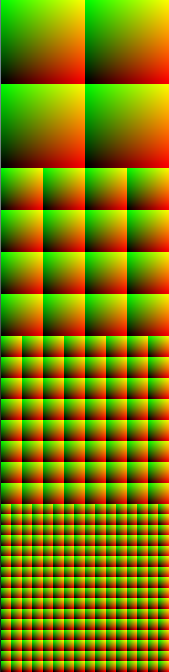
\includegraphics[height=\columnwidth, angle=-90]{images/surface_cascades.png}
  \caption{\label{fig:surface_cascades}
     An example of surface radiance cascade hierarchy: cascade 0 on the left has 16x16 probes, each with 8x8 resolution, cascade 1 has 8x8 probes each with 16x16 resolution, etc. Width of this atlas grows linearly with the number of cascades.}
\end{figure}

\subsection{Calculating indirect lighting with radiance cascades}
Once radiance cascades are calculated, they can be used to calculate an approximation of the rendering equation \cref{eqn:rendering} that gives outgoing/exitant radiance or the final "visible" color of a render surface.

This equation can be calculated numerically in a naive way, by sampling a set of directions for each point, and querying $L_{\mathrm{in}}$ from the radiance cascades. However, it can be done much more efficiently by introducing a very small amount of bias for some of the common BRDF's.

For calculating diffuse lighting (irradiance), it's possible to merge all cascades $N-1..0$ onto cascade 0 and then calculate the integral using its relatively few discrete directions. This can be done efficiently, because projecting cascade $i+1$ onto cascade $i$ can be done quite cheaply by just averaging 2 or 4 texels of cascade $i+1$ and merging the result with a texel of cascade $i$, at the end of such chain cascade 0 will contain an approximation of full radiance for an entire solid angle corresponding to each of its probes' texels. The reason why approach introduces only a small bias for diffuse lighting is because the multiplier under the integral $ f(\textbf p, \hat \omega_\mathrm{in}, \hat{\omega}_\mathrm{out}) \cdot |\hat{n} \cdot \hat{\omega}_\mathrm{in} |$ has a very low directional frequency, so the integral can be calculated efficiently by having just a few samples of incoming radiance averaged over relatively large cones.

Specular lighting can be approximated by incoming radiance averaged over a single cone in the direction of reflected view vector with its angle defined by the surface roughness. Averaging radiance over a cone can be done using radiance cascades in $O(N)$ where $N$ is the number of cascades. Minimum angle of a cone approximated with radiance cascades can be achieved by querying a radiance interval from each cascade individually and then merging all such intervals: this results in an approximation of radiance cone with an angle equal to directional step of cascade $N$.  Maximum angle of a cone can be achieved by merging all cascades first and then querying a single direction from merged cascade 0: this will result in a wide cone corresponding to directional step of cascade 0. And every intermediate value of radiance cone angle can be achieved by querying $0..K$ radiance intervals from individual cascades, then merging the remaining $K+1..N$ and merging the result with a single query from a merged cascade $K$.

\section{Analysis}

For the sake of brevity, let's limit detailed analysis to the case of flatland, as it is also applicable to the screenspace implementation and that is the encoding used in Path of Exile 2.
Let's assume that cascade 0 has a total of $P_0$ probes and each probe stores $Q_0$ discrete values corresponding to $M_0$ uniformly distributed directions in image space. This means that cascade 0 encodes a total of $M_0=P_0Q_0$ radiance intervals in the range of $[0..t_0]$. Now, let's add another cascade, cascade 1. As discussed earlier, cascade 1 would have half the number of probes along each spatial dimension, $P_1=P_0/4$ probes total, but each probe would store two times more discrete values $Q_1=2Q_0$, which allows storing total of $M_1=P_1Q_1=P_0Q_0/2$ of radiance intervals in the range of $[t_0,t_1]=[t_0,2t_0]$ for cascade 1.


\begin{figure}[htb]
  \centering
  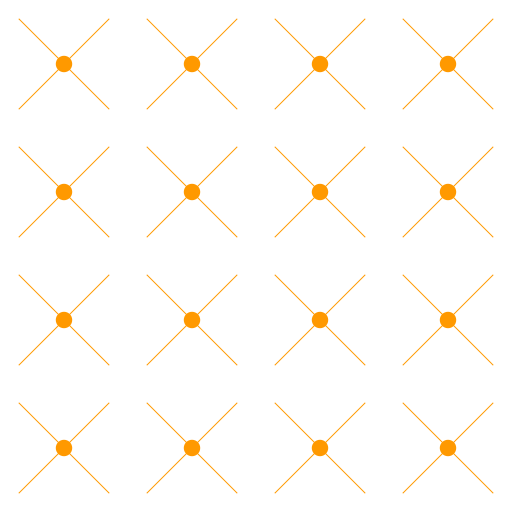
\includegraphics[width=0.49\columnwidth]{images/cascade 0.png}
  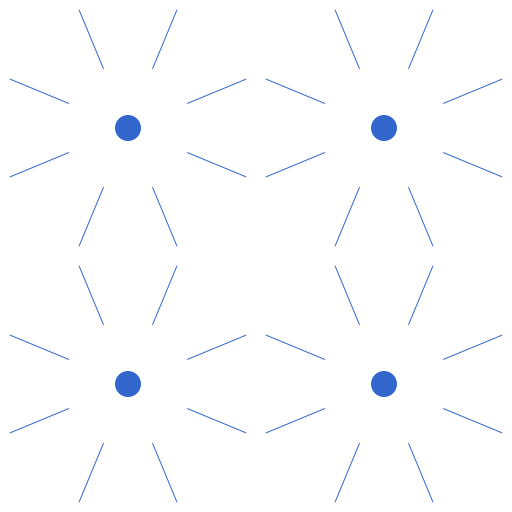
\includegraphics[width=0.49\columnwidth]{images/cascade 1.png}
  \caption{\label{fig:cascades}
     Schematic visualization of two \emph{radiance cascades}. Left: cascade 0 contains 16 total with 4 values of radiance interval stored in each. Right: cascade 1 contains 4 probes with 8 values of radiance interval stored in each.}
\end{figure}


Now, since data in each of these cascades is interpolateable, it is possible to interpolate radiance interval with range $[t_1, t_2]=[t_0,2t_0]$ in cascade 1 onto position of each probe in cascade 0($P_0$ positions total), and
it is also possible to calculate radiance interval $[0,t_0]$ of cascade 0 onto every probe direction ($Q_1=2Q_0$ total) used in cascade 1.



This allows constructing total of $P_0Q_1=2P_0Q_0$ radiance intervals of range $[0,t_1]$. A keen observer might notice something strange at this point: cascade 0 contains $P_0Q_0$ radiance intervals,
cascade 1 contains $P_0Q_0/2$ radiance intervals, but combining them produces $2P_0Q_0$ radiance intervals, instead of $P_0Q_0+P_0Q_0/2=\frac{3}{2}P_0Q_0$ intervals. And adding yet another cascade (cascade 2) requires calculating
$P_2Q_2=P_0Q_0/4$ more radiance intervals in the range of $[t1,t2]=[2t_0,4t_0]$, but then allows constructing $4P_0Q_0$ radiance intervals in the range of $[0,4t_0]$.

\begin{figure}[htb]
  \centering
  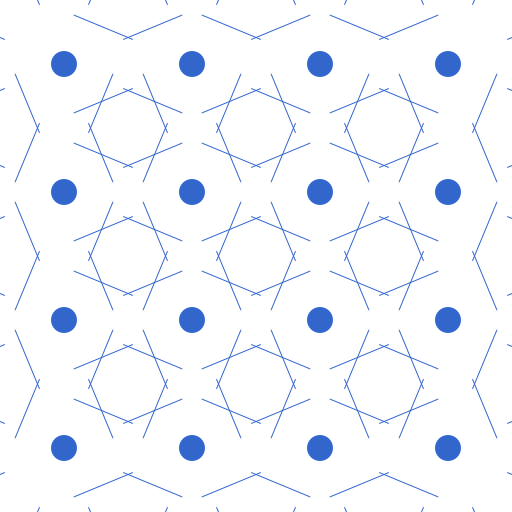
\includegraphics[width=0.49\columnwidth]{images/cascade 1 on 0 exclusive.png}
  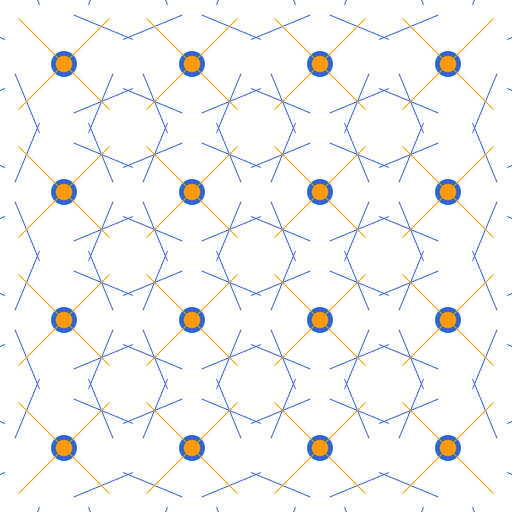
\includegraphics[width=0.49\columnwidth]{images/cascade 1 on 0 merged.png}
  \caption{\label{fig:cascades}
     Left: cascade 1 radiance interval interpolated for every position of probe in cascade 0; Right: cascade 0 merged with interpolated intervals of cascade 1.}
\end{figure}

\begin{figure}[htb]
  \centering
  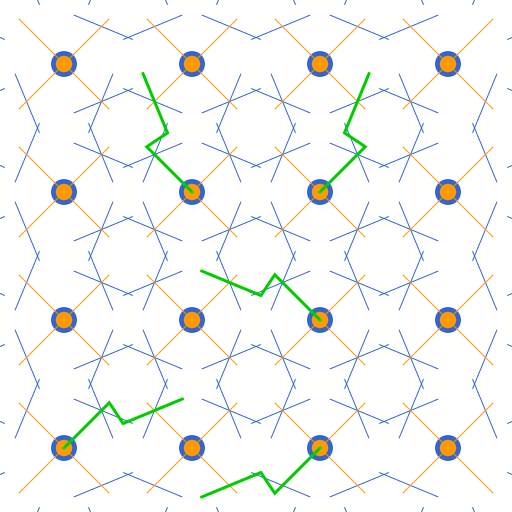
\includegraphics[width=0.49\columnwidth]{images/cascade 1 on 0 rays.png}
  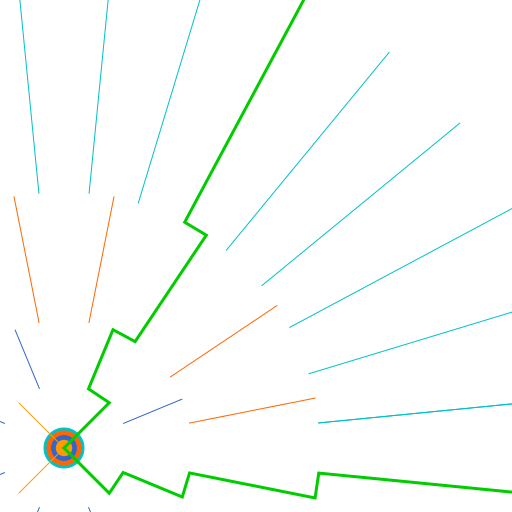
\includegraphics[width=0.49\columnwidth]{images/max rays.png}
  \caption{\label{fig:cascades}
     Left: highlighted in green are 5 out of 128 merged radiance intervals that can be constructed by combining intervals stored in cascade 0 and interpolated intervals of cascade 1 Right: highlighted 2 out 64 possible merged radiance intervals \emph{per every cascade 0 probe} after combining 4 cascades total.}
\end{figure}
%

This means that adding one more cascade always costs half as much as adding the previous one (both in terms of memory storage as well as calculation cost), but effectively increases the number of approximated maximum-range radiance intervals twice. Since each maximum range interval serves is basically equivalent to casting another ray, it means that adding each cascade increases the number of rays total twice, while being half the cost of the previous one. Compare this with classic path tracing that requires paying twice greater cost to cast twice more rays.

In other words, the total number of rays equivalent to having $N$ radiance cascades increases exponentially with $N$, while the total cost needed to calculate and store them stays less than twice the cost of cascade 0:
\begin{equation}
  \begin{cases}
    \text{rays}(N) = 2^N\text{rays}(0); \\
    \text{cost}(N) = (1+1/2+...+1/2^N)\text{cost}(0)<2\text{cost}(0).
  \end{cases}
  \label{eq:scaling}
\end{equation}

This is also equivalent to saying that an infinite number of rays can be calculated in a finite amount of time. Now, there's obviously a certain amount of facetiousness to this statement, because the number of cascades can not actually be greater than $\log(P_0)$ due to their discrete nature.
Another small caveat is that constructed radiance intervals are assembled from interpolated parts, and such construction will not introduce a significant error if and only if the penumbra hypothesis holds. That being said, the seemingly unbelievable quality of exponential scaling for a constant cost does indeed hold in reality.

What this analysis means is that with radiance cascades the total number of rays is basically no longer a limiting factor of calculating global illumination. It is important to note that it does not mean it automatically solves the problem of global illumination once and for all. First, there's still a couple technical aspects that need attention: how exactly to calculate data of every radiance cascade, how exactly to calculate irradiance from radiance efficiently enough, how to go from 2d flatland radiance cascades to storing 3d screenspace data, etc. And secondly, a unique type of problems can indeed arise, once the fundamental assumption, \emph{the penumbra hypothesis} starts breaking down. This happens if one tries to encode a point light that is just too small or to encode a penumbra that is too sharp, or chooses incorrectly one of the parameters, such as cascade 0 probe linear/angular stepping or its range (so any of $P_0$, $Q_0$ or $t_0$). But the practice has shown that it is indeed
possible to find the right range of these parameters for most applications so that the penumbra hypothesis does hold and radiance cascades do scale in this seemingly impossible way in practice.
\section{Implementations}
At the time of writing this article, there are 4 implementations that use \emph{radiance cascades} for practical applications and for research purposes. Each of them is detailed in its own subsection down below.

\subsection{Radiant 2d}
\begin{figure}[htb]
  \centering
  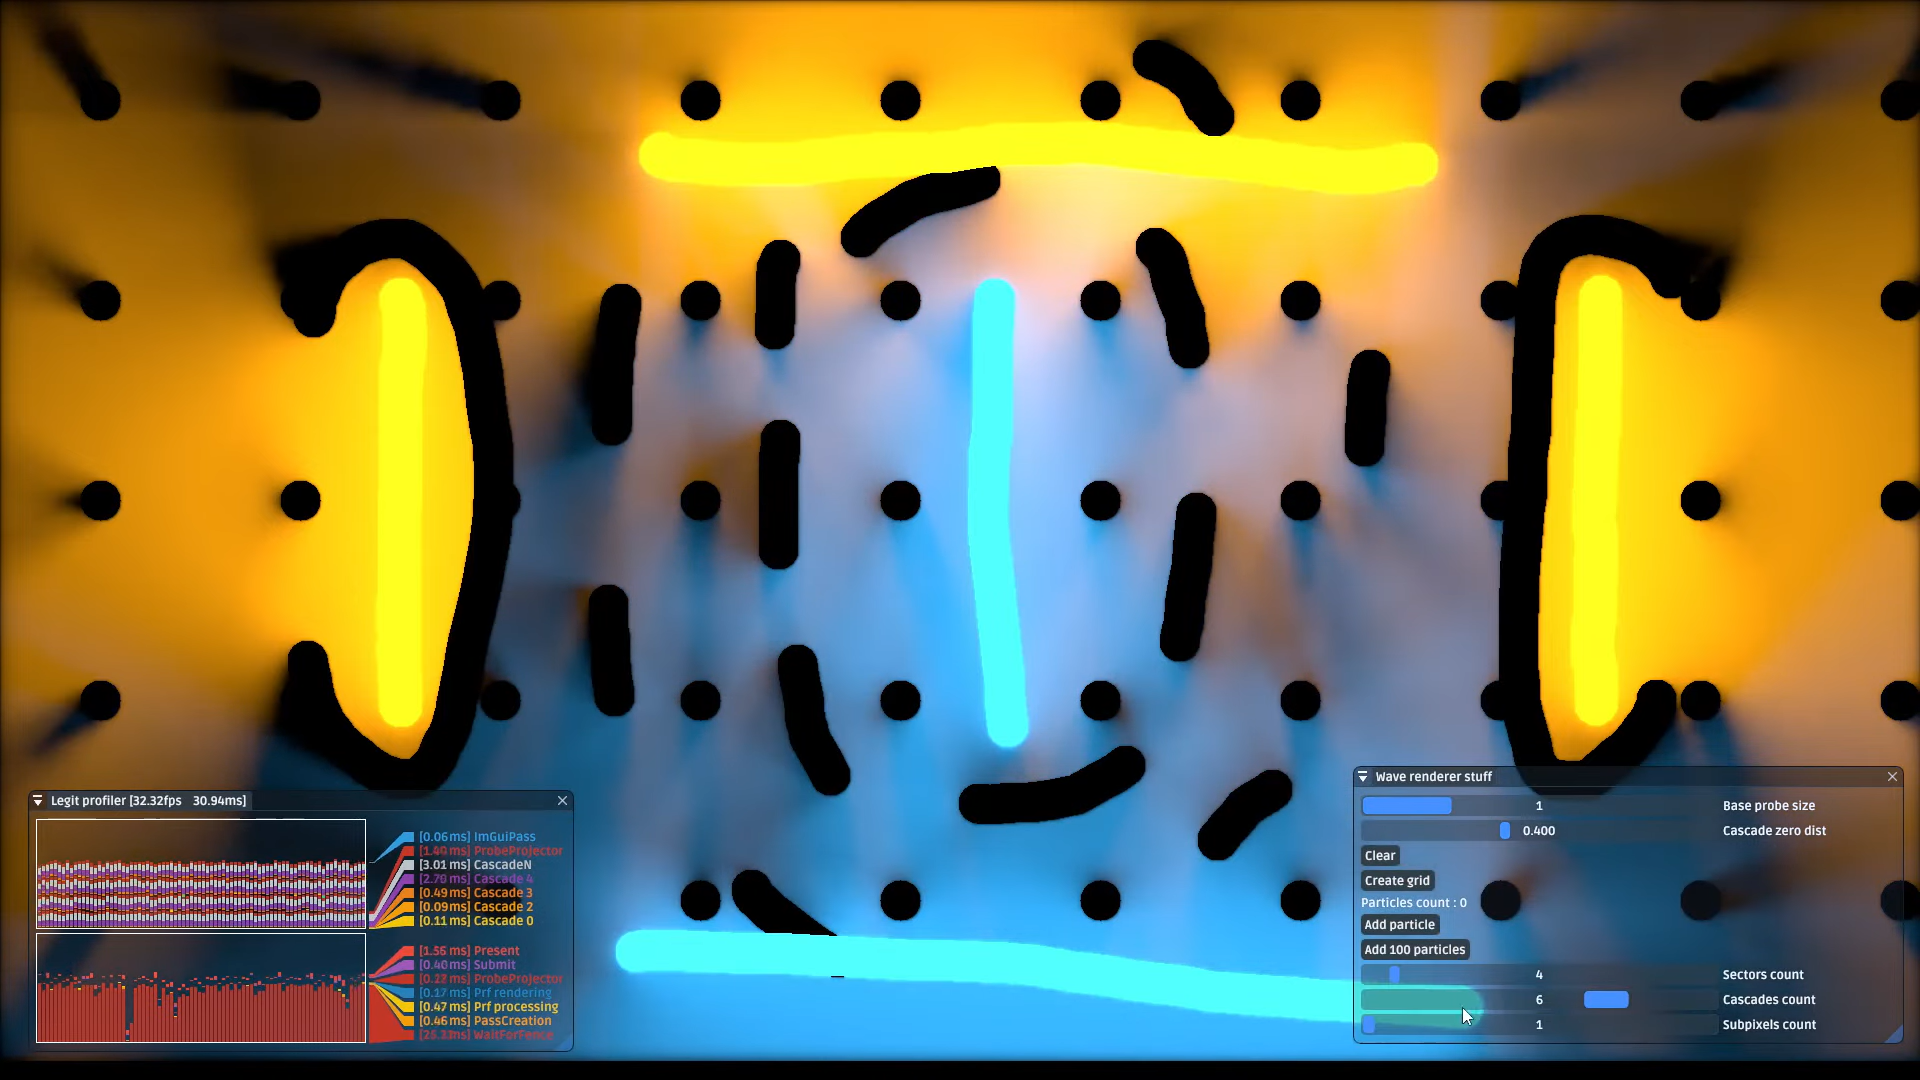
\includegraphics[width=\columnwidth]{images/gi_2d.png}
  \caption{\label{fig:radiant_2d}
     The first proof of concept implementation of radiance cascades in 2d.}
\end{figure}
\emph{Radiant 2d} is my first implementation of \emph{radiance cascades} that proved such a concept can indeed work. \emph{Radiant 2d} is capable of calculating per-pixel global illumination in 2d in a constant time of about 30ms on a GTX3060, depending on required fidelity. Its cost is completely fixed and is entirely scene-independent, which is shown on Figure \ref{fig:flatland_scaling}.

\begin{figure}[htb]
  \centering
  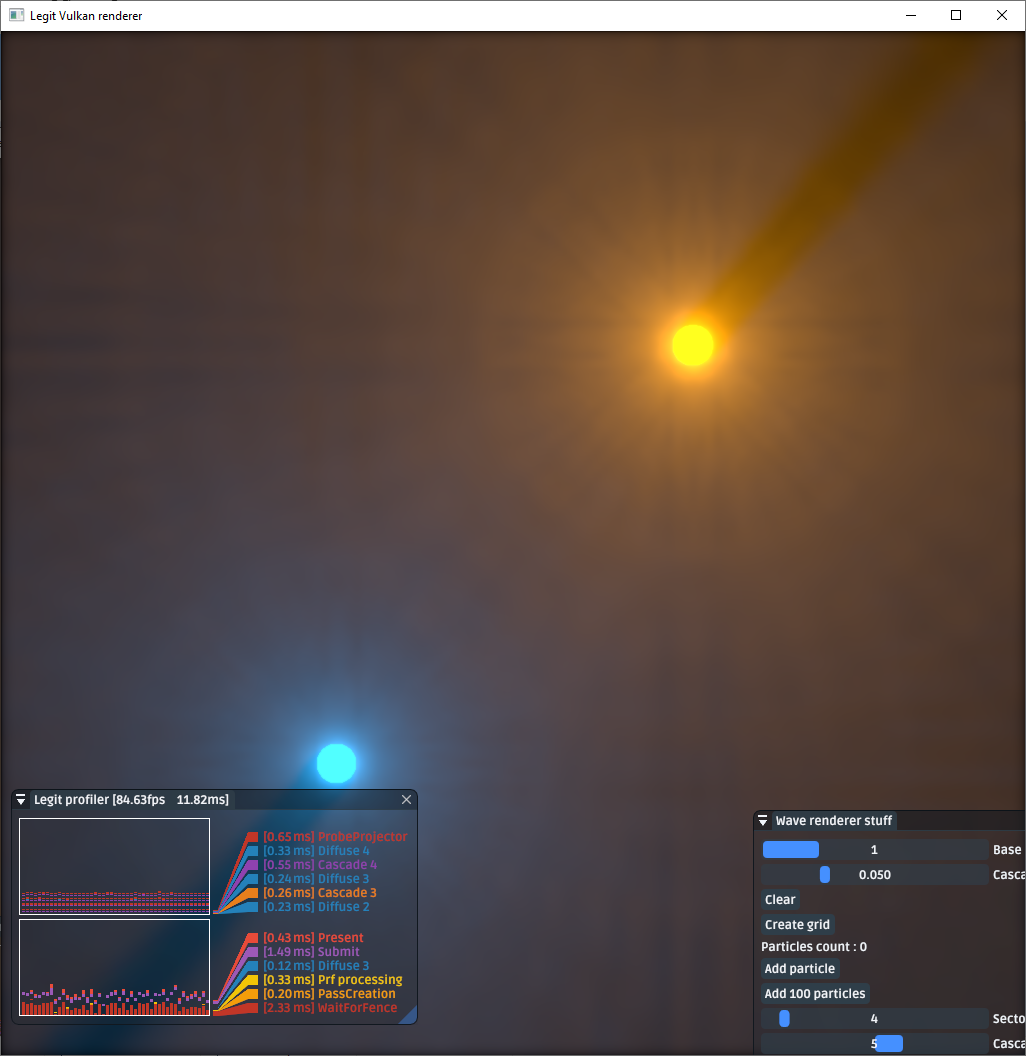
\includegraphics[width=0.32\columnwidth]{images/flatland_2_particles_1024.png}
  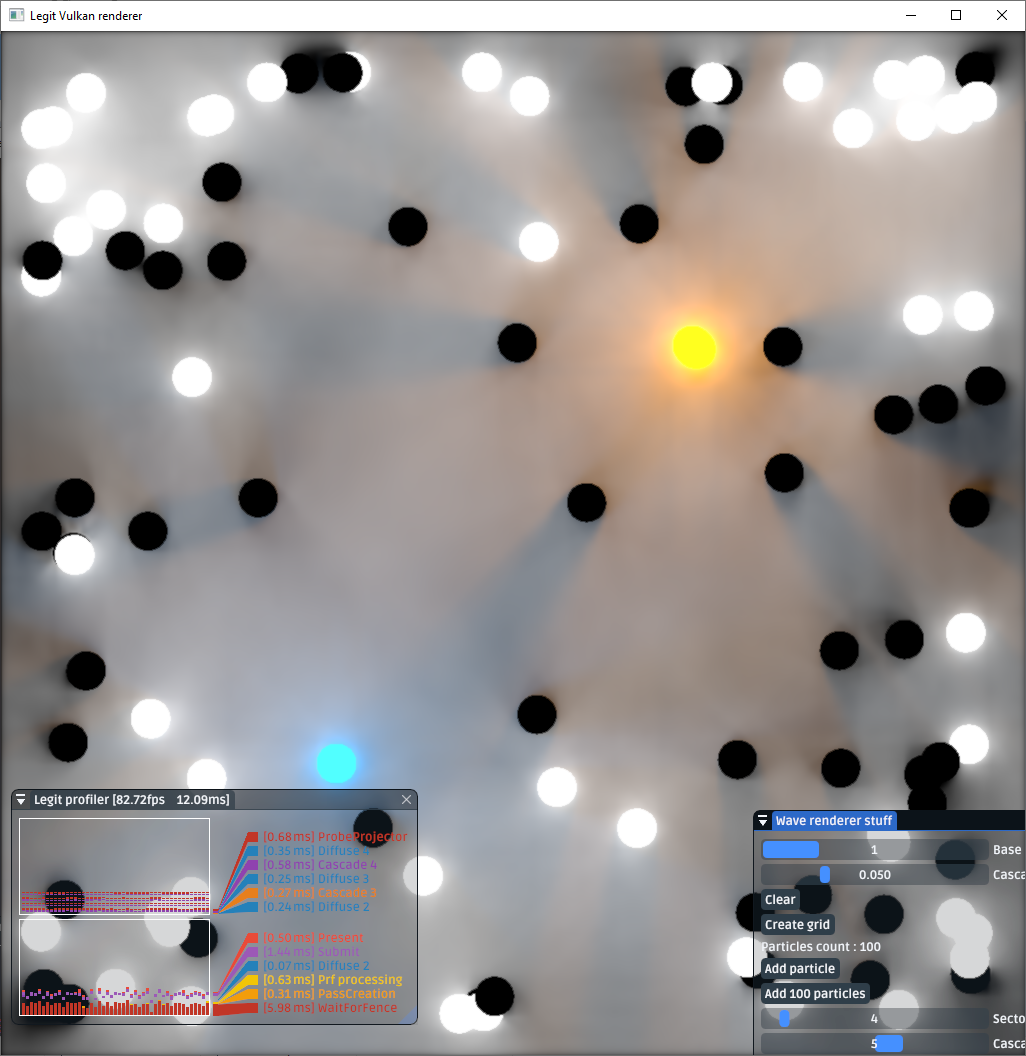
\includegraphics[width=0.32\columnwidth]{images/flatland_102_particles_1024.png}
  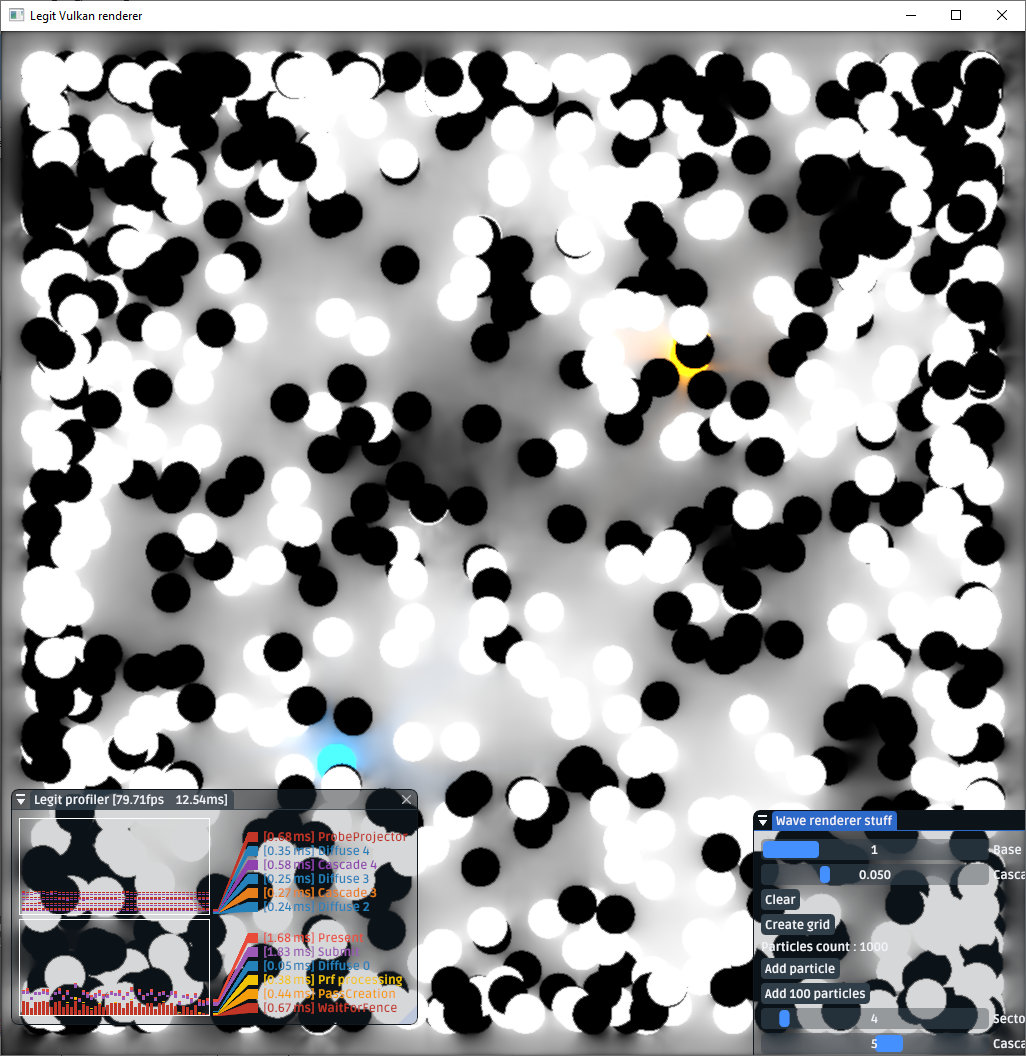
\includegraphics[width=0.32\columnwidth]{images/flatland_1002_particles_1024.png}
  \caption{\label{fig:flatland_scaling}
     Radiance cascades are completely scene-independent and calculate lighting for 2, 102 and 1002 particles in the same amount of time of about 12ms.}
\end{figure}

It is curious to see what calculated global illumination looks like depending on the radiance interval range of cascade 0 (a reminder, this is an arbitrary parameter that all subsequent cascades scale off). A Figure \ref{fig:flatland_range_scaling} shows how radiance intervals from different cascades blend into a smooth and continuous radiance approximation.
\begin{figure}[htb]
  \centering
  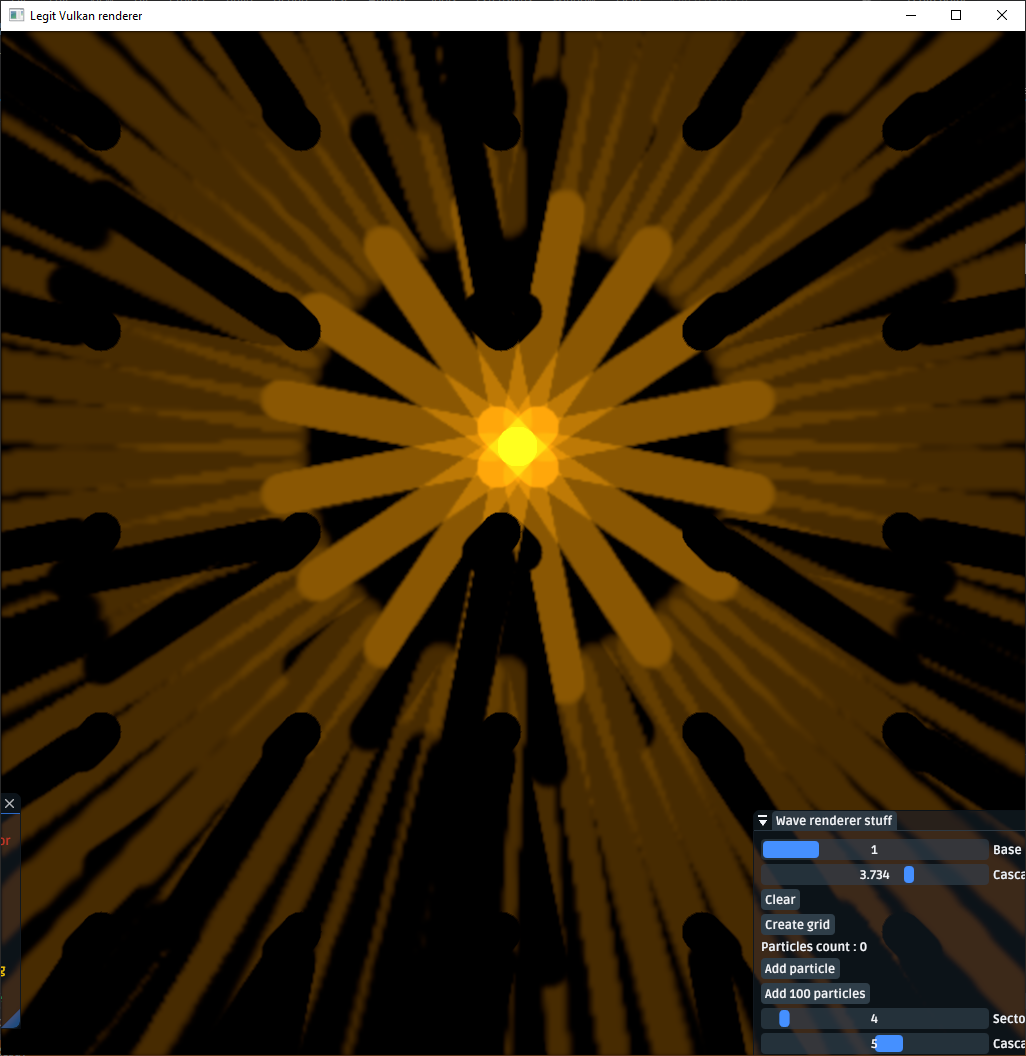
\includegraphics[width=0.32\columnwidth]{images/flatland_mult_3.png}
  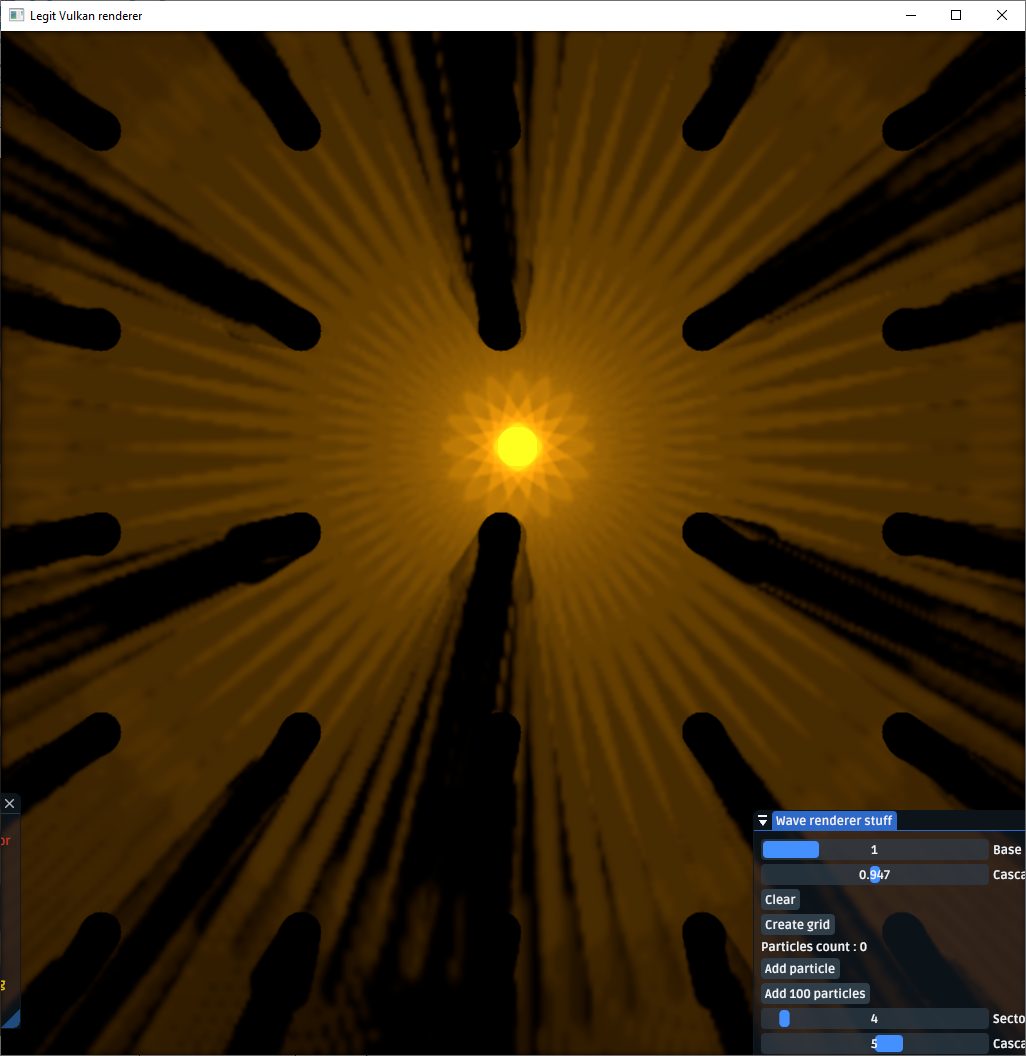
\includegraphics[width=0.32\columnwidth]{images/flatland_mult_2.png}
  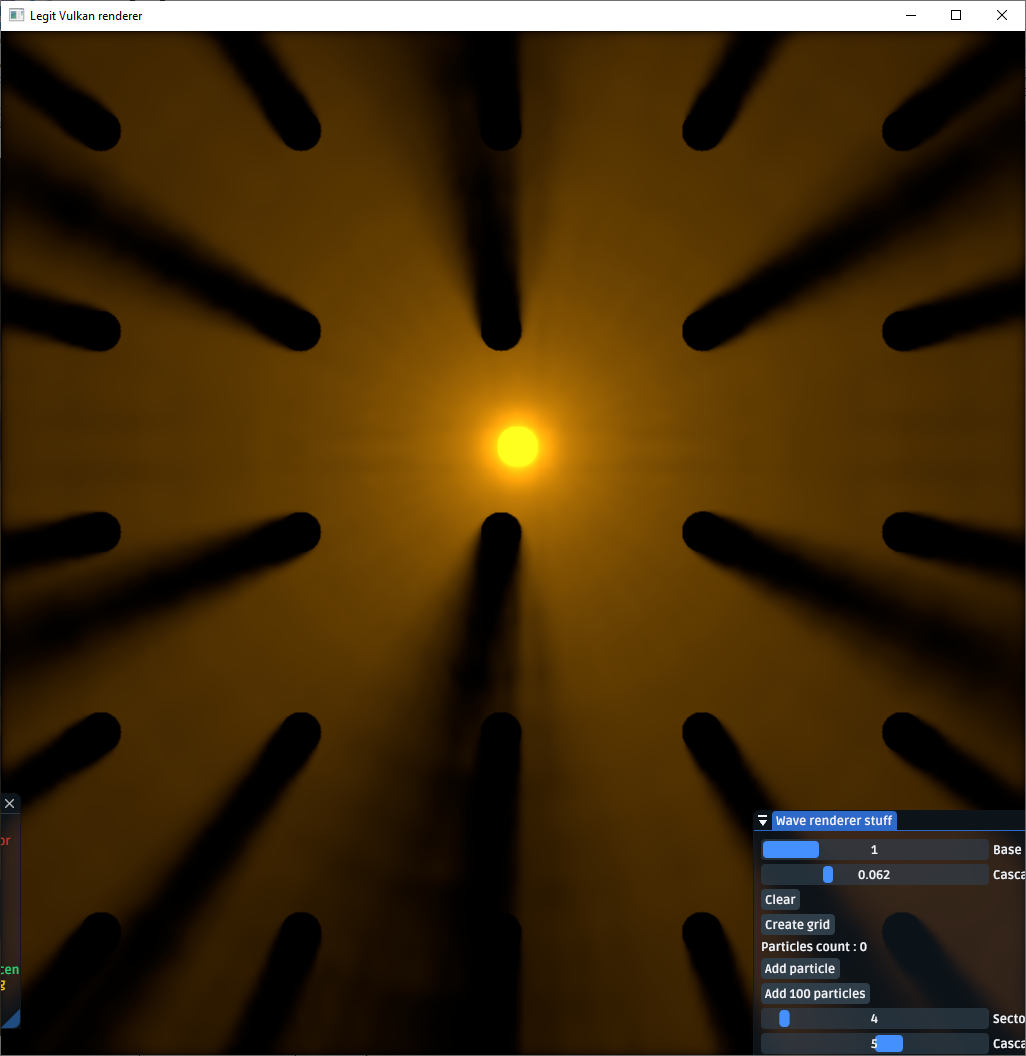
\includegraphics[width=0.32\columnwidth]{images/flatland_mult_1.png}
  \caption{\label{fig:flatland_range_scaling}
     From left to right the sequence shows what it looks like to decrease the range associated with cascade 0. The first image shows very crude and disconnected radiance intervals that connect smoother with decreased cascade 0 range and finally connect into a continuous radiance approximation once the range is small enough on the right image.}
\end{figure}

Radiant 2d also utilizes an interesting way of calculating radiance intervals \emph{within} every cascade. It relies on the fact that any radiance interval can be extended with itself, essentially doubling its corresponding range, using formula \ref{eq:extending_intervals}. Instead of calculating long range radiance interval of, say $[512, 1024]$ pixels, it calculates a radiance interval of $[512, 512+32]$, then extends it to $[512, 512+64]$ and so on until it reaches the target $[512, 512+512]$. This is possible specifically for representations that use rectilinear grids of radiance interval probes (so flatland and 3d world space cascades) and unfortunately not possible for 3d screenspace cascades where every probe has its own depth value.

For the sake of completeness and further research it is worth mentioning that Radiant 2d used a slightly different scaling law than what's described in Section \ref{sub:flatland_scaling}. As can be seen on figure \ref{fig:flatland_range_scaling}, each subsequent cascade has 4x higher angular resolution instead of 2x increase as discussed in Section \ref{sub:flatland_scaling}. This way all cascades are encoded with the same amount of storage, similar to how 3d surface fields scale as discussed in Section \ref{sub:surface_scaling}. This scheme seemingly produced higher quality:cost ratio and it remains to be seen whether it was a fluke of my original implementation or there's some fundamental property hidden behind this fact.
\subsection{Path of Exile 2 GI}
\emph{Path of Exile 2}'s new GI solution is the main implementation of this work. It uses a hierarchy of screenspace radiance probe cascades that are populated with screenspace raymarching.

\begin{figure}[htb]
  \centering
  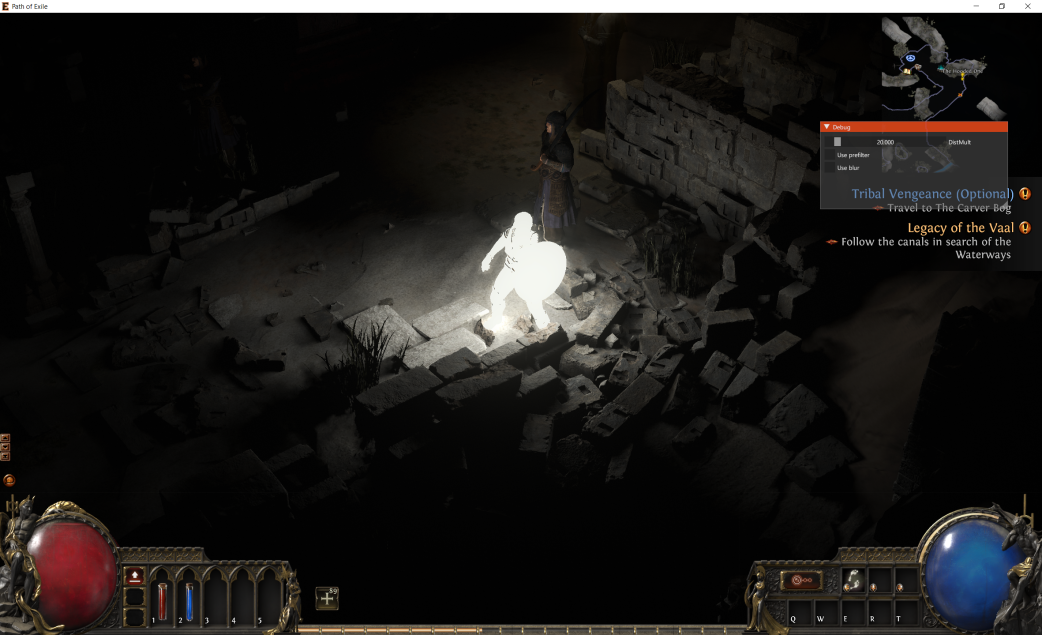
\includegraphics[width=\columnwidth]{images/ranger_gi.png}
  \caption{\label{fig:ranger_gi}
     Implementation of radiance cascades in Path of Exile 2, running in ~3ms on GTX1050 and used to calculate indirect light coming from a glowing character.}
\end{figure}
In order to make it possible to run on the target hardware, PoE2 GI uses a very efficient screenspace raymarching scheme that instead of casting individual rays corresponding to each radiance interval, it raymarches 4 rays simultaneously, basically for free and stores occlusion in 128-bit bitmask, that is equivalent to storing 128 binary occlusion rays per radiance cascade texel. There's a lot to be said about this implementation, however it is unfortunately outside of the scope of this article which has the basic concept of radiance cascades as its main focus.

\begin{figure}[htb]
  \centering
  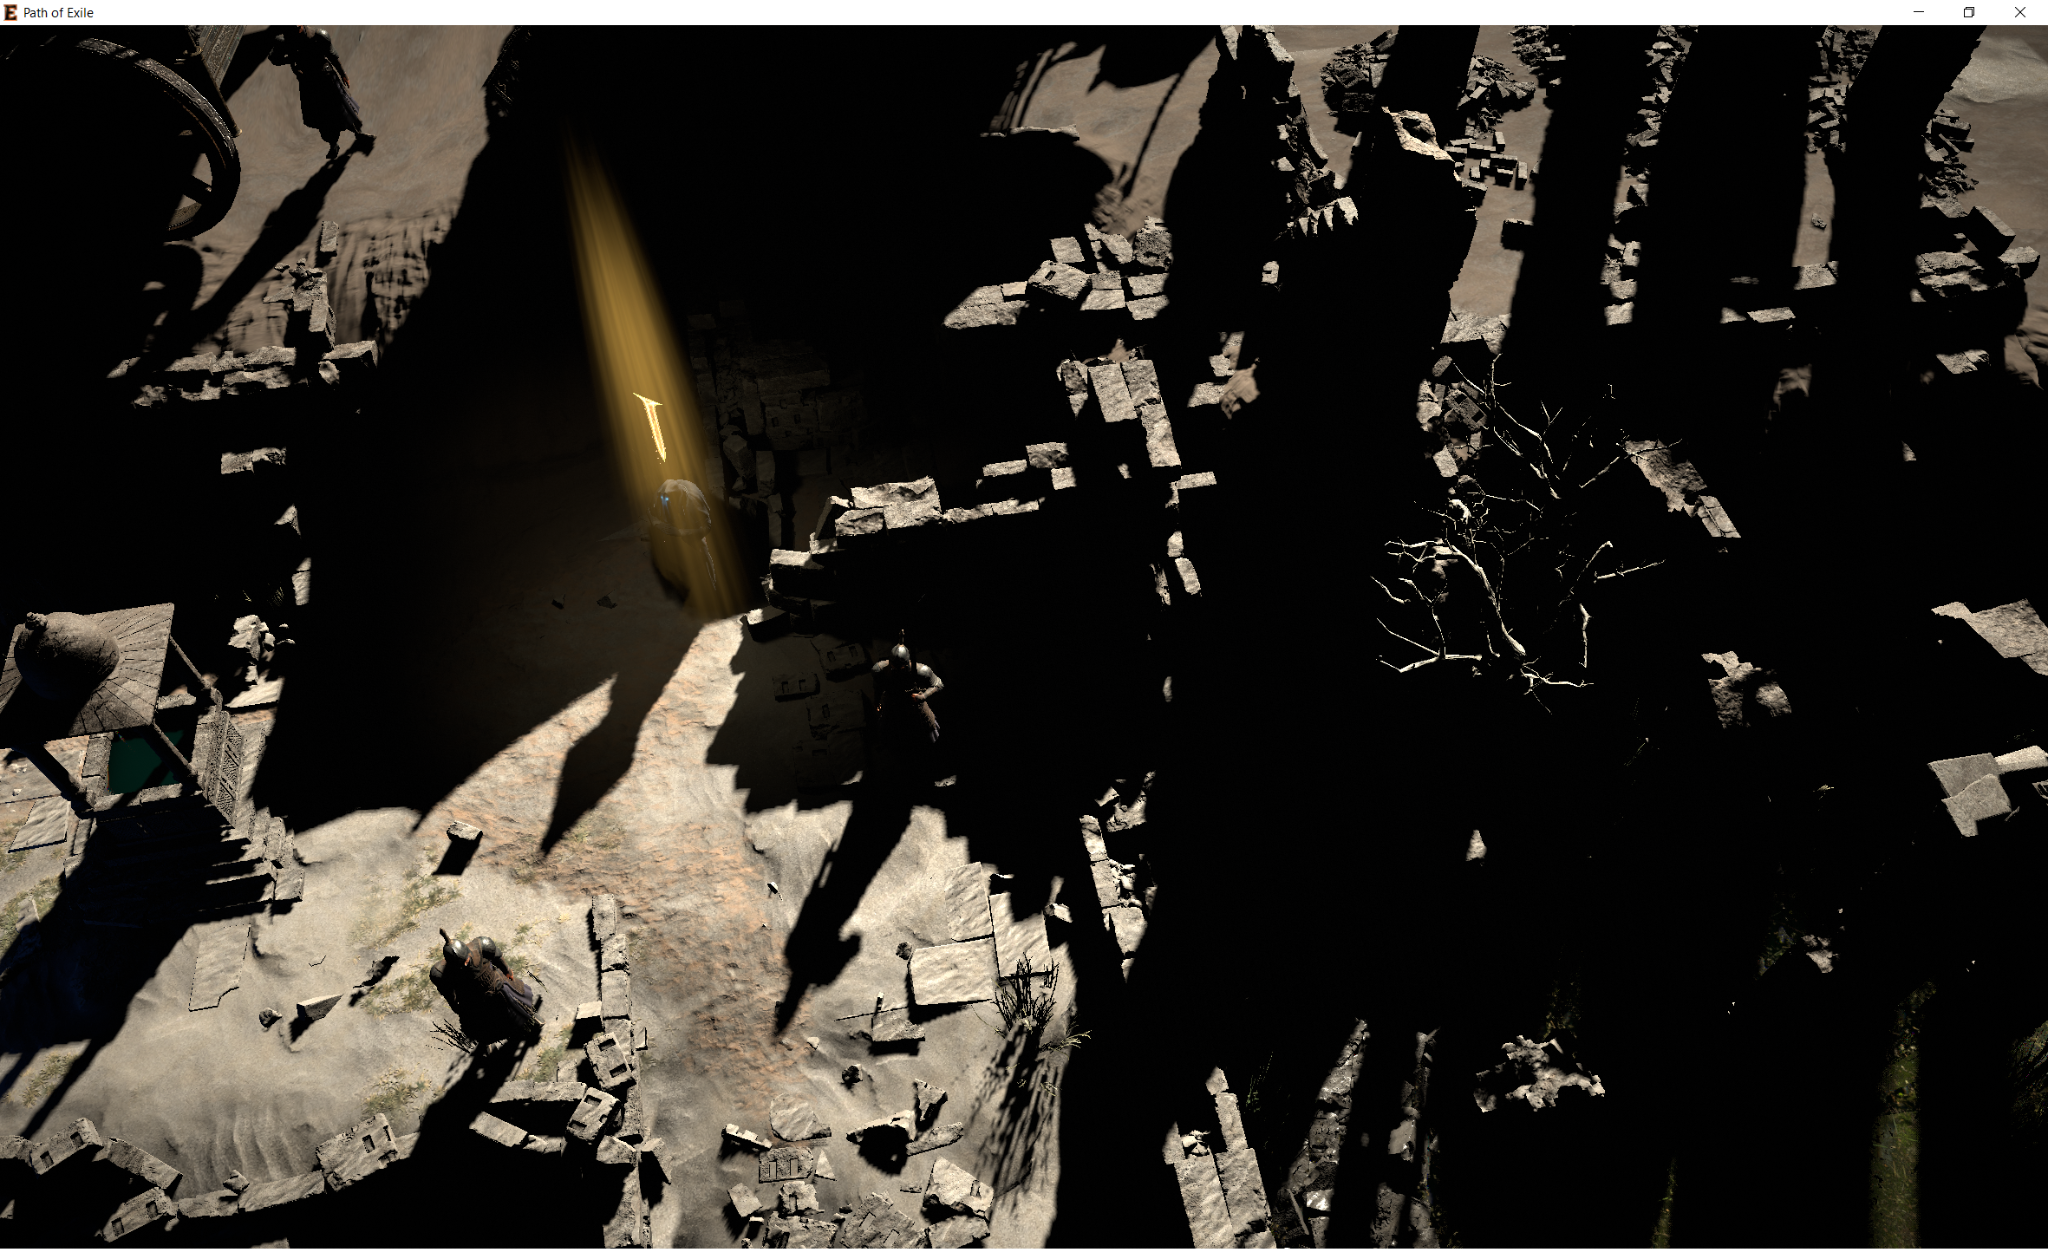
\includegraphics[width=\columnwidth]{images/poe2_gi_off.png}
  \includegraphics[width=\columnwidth]{images/poe2_gi_on.png}
  \caption{\label{fig:poe_gi_onoff}
     Comparison of Path of Exile 2 running with gi off and on.}
\end{figure}


Since radiance cascades encode the entire light field information, they combine particularly well with normal mapping, providing accurate directional lighting. In addition, directional distribution of radiance can be convolved with an arbitrary BRDF/BSDF to achieve specular lighting, refraction, complex microsurface distributions, etc. An example of radiance cascades used for specular only lighting is shown on Figure \ref{fig:poe_specular} and combined diffuse+specular can be seen on Figure \ref{fig:poe_spec_and_diff}.

\begin{figure}[htb]
  \centering
  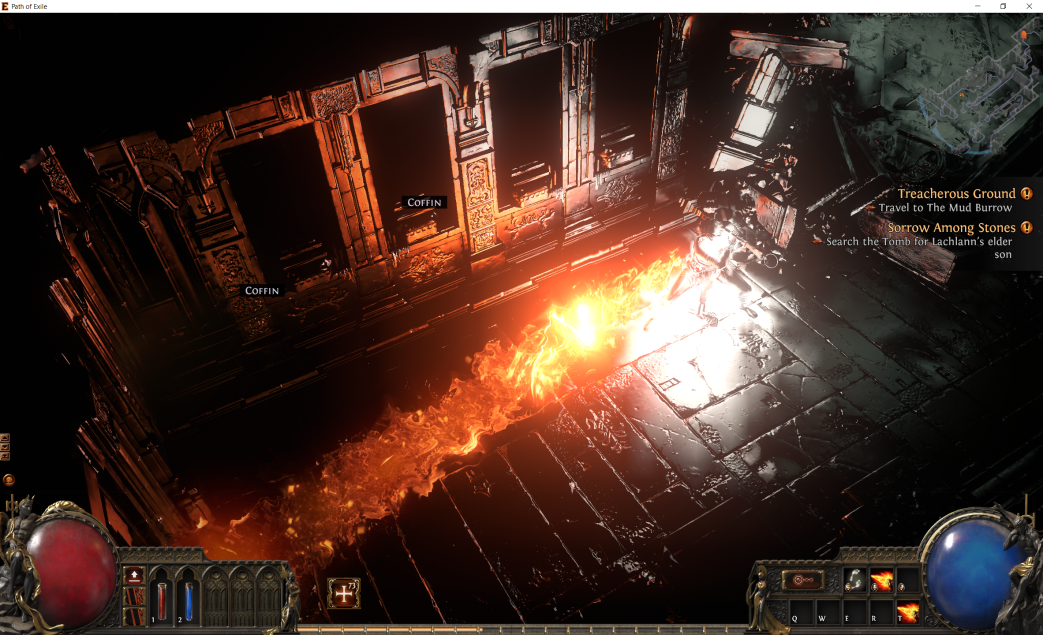
\includegraphics[width=\columnwidth]{images/poe2_reflections_1.png}
  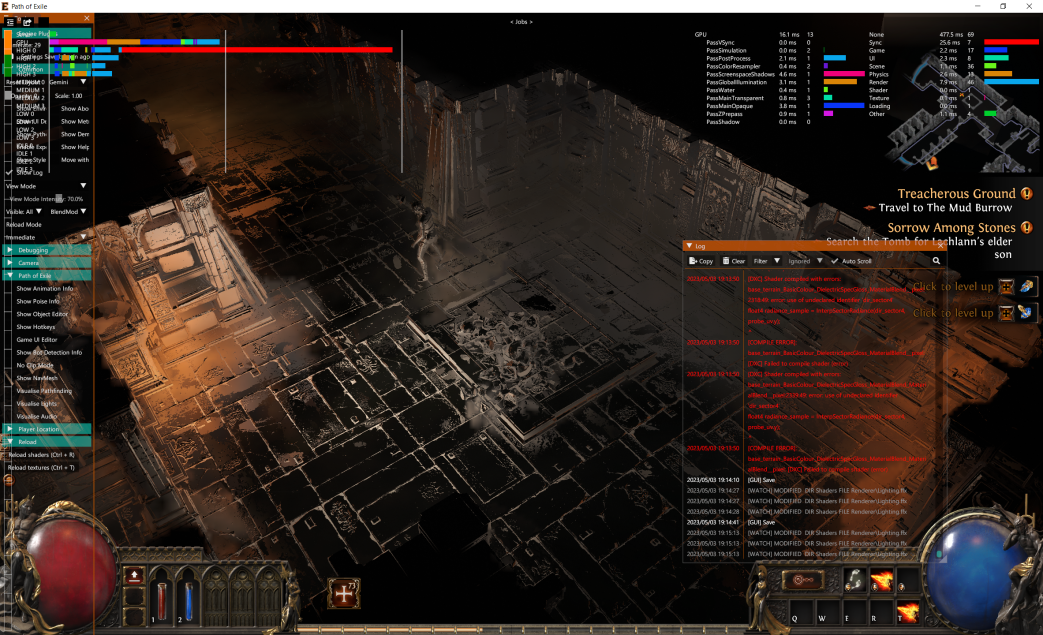
\includegraphics[width=\columnwidth]{images/poe2_reflections_2.png}
  \caption{\label{fig:poe_specular}
     An experiment where radiance cascades are used to render specular glossy materials (specular only).}
\end{figure}

\begin{figure}[htb]
  \centering
  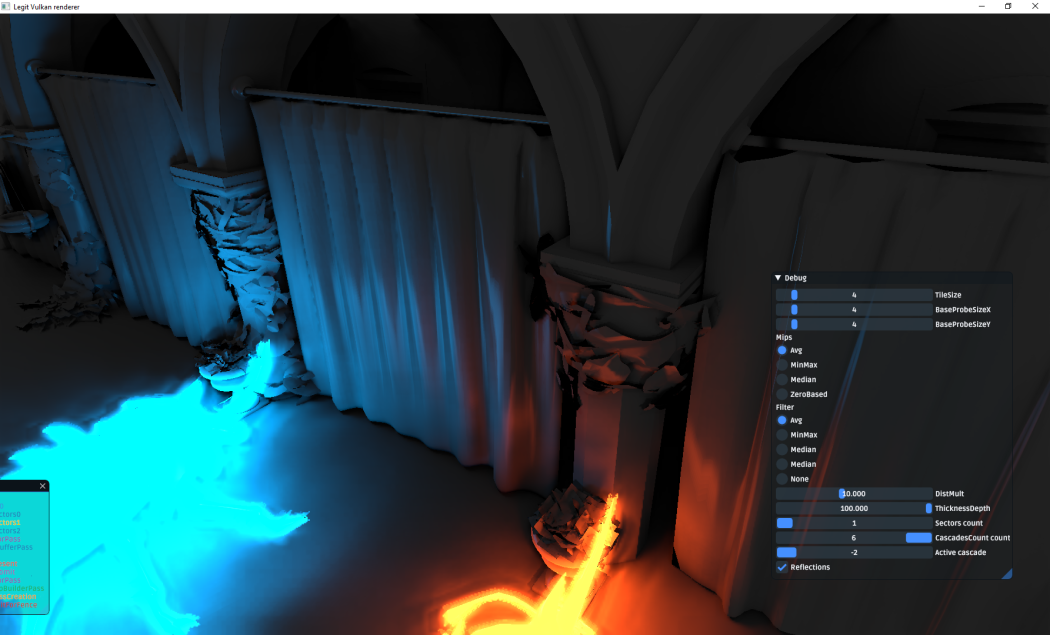
\includegraphics[width=\columnwidth]{images/radiant_specular.png}
  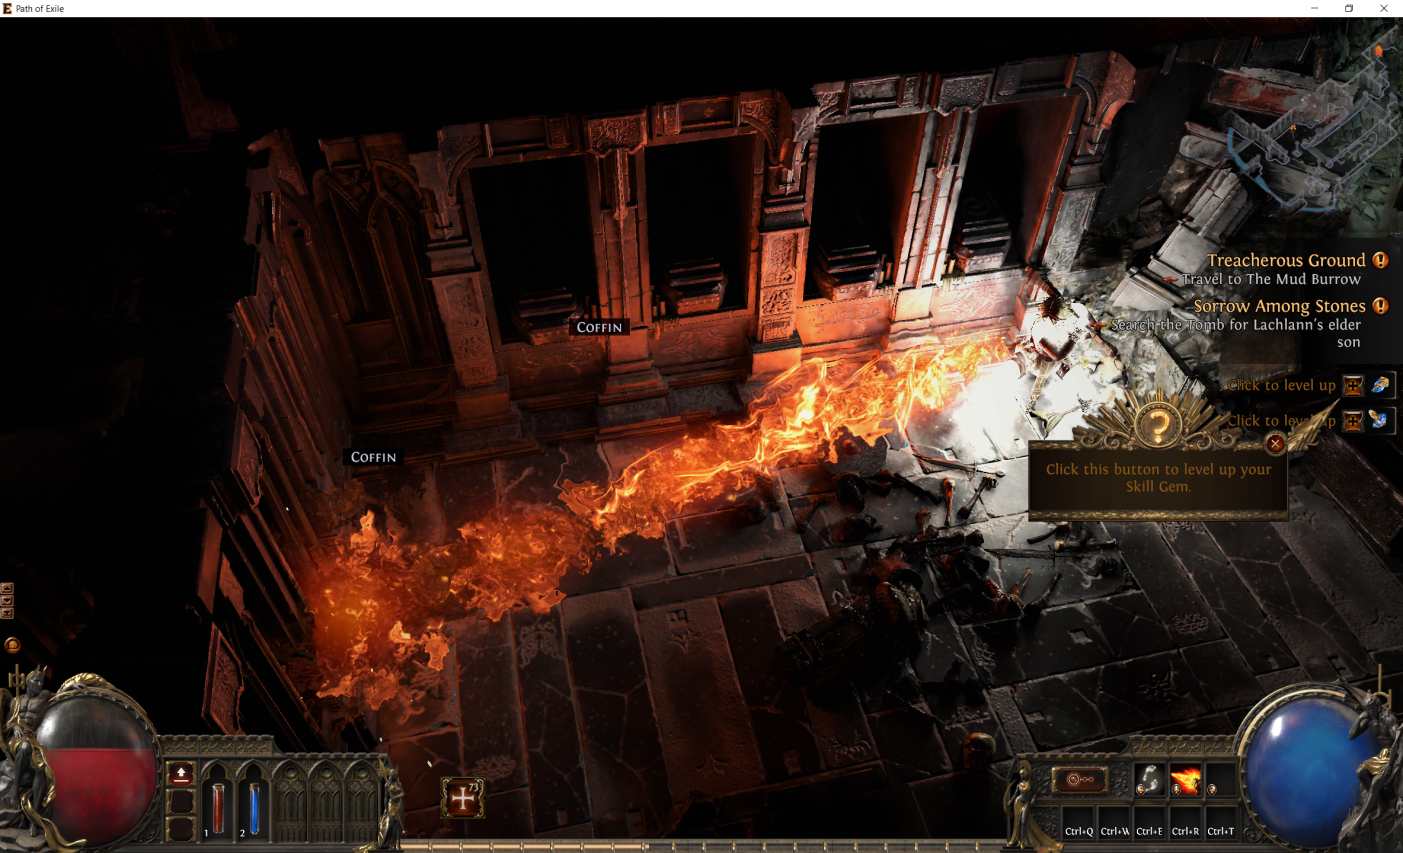
\includegraphics[width=\columnwidth]{images/poe2_reflections_comb.png}
  \caption{\label{fig:poe_spec_and_diff}
     Combined diffuse+specular lighting calculated using only emissive materials stored in radiance cascades.}
\end{figure}


\clearpage
\subsection{Radiance 3d}
\emph{Radiance 3d} is an experimental testbed designed to investigate properties of world space radiance cascades. It utilizes a 3d regular grid of radiance probes encoded in a volume texture, uses a 3d voxelization.

\begin{figure}[htb]
  \centering
  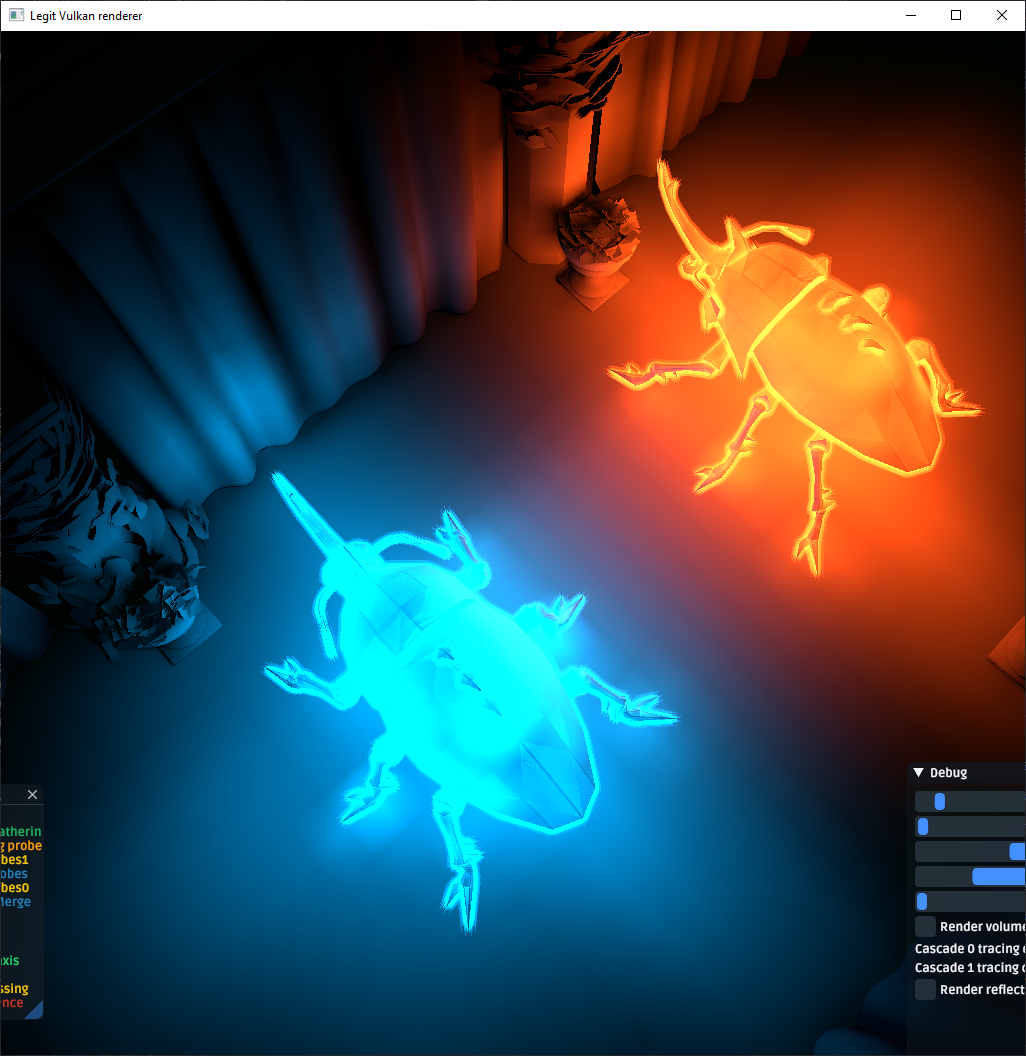
\includegraphics[width=0.49\columnwidth]{images/radiance_3d_from_voxels.png}
  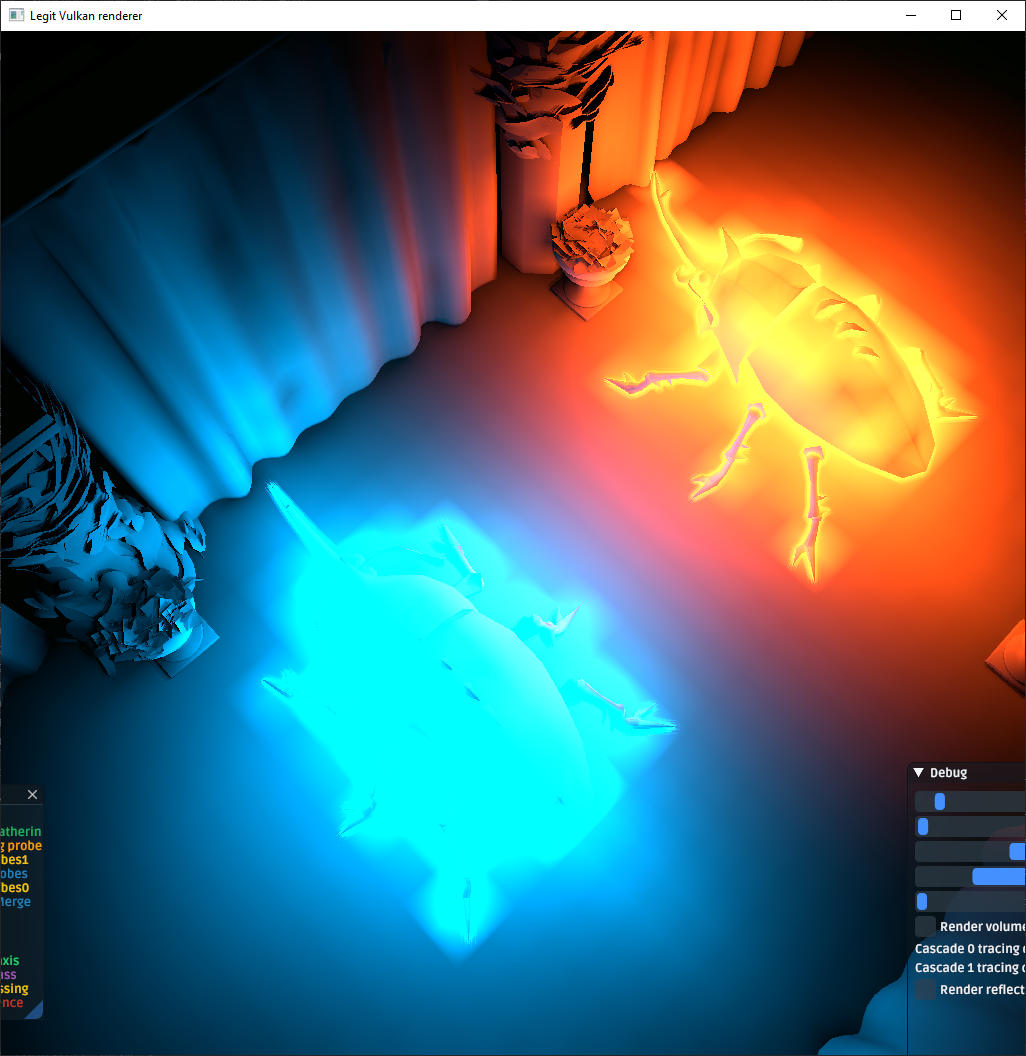
\includegraphics[width=0.49\columnwidth]{images/radiance_3d_from_screenspace.png}
  \caption{\label{fig:radiance_3d_voxels}
     Comparison between world space 3d radiance cascades using either screenspace data for radiance interval calculation(left) or voxelized world space data(right).}
\end{figure}

The version of this implementation that uses world space voxelization is done entirely in world space, which is illustrated in Figure \ref{fig:radiance_3d_offscreen}.
\begin{figure}[htb]
  \centering
  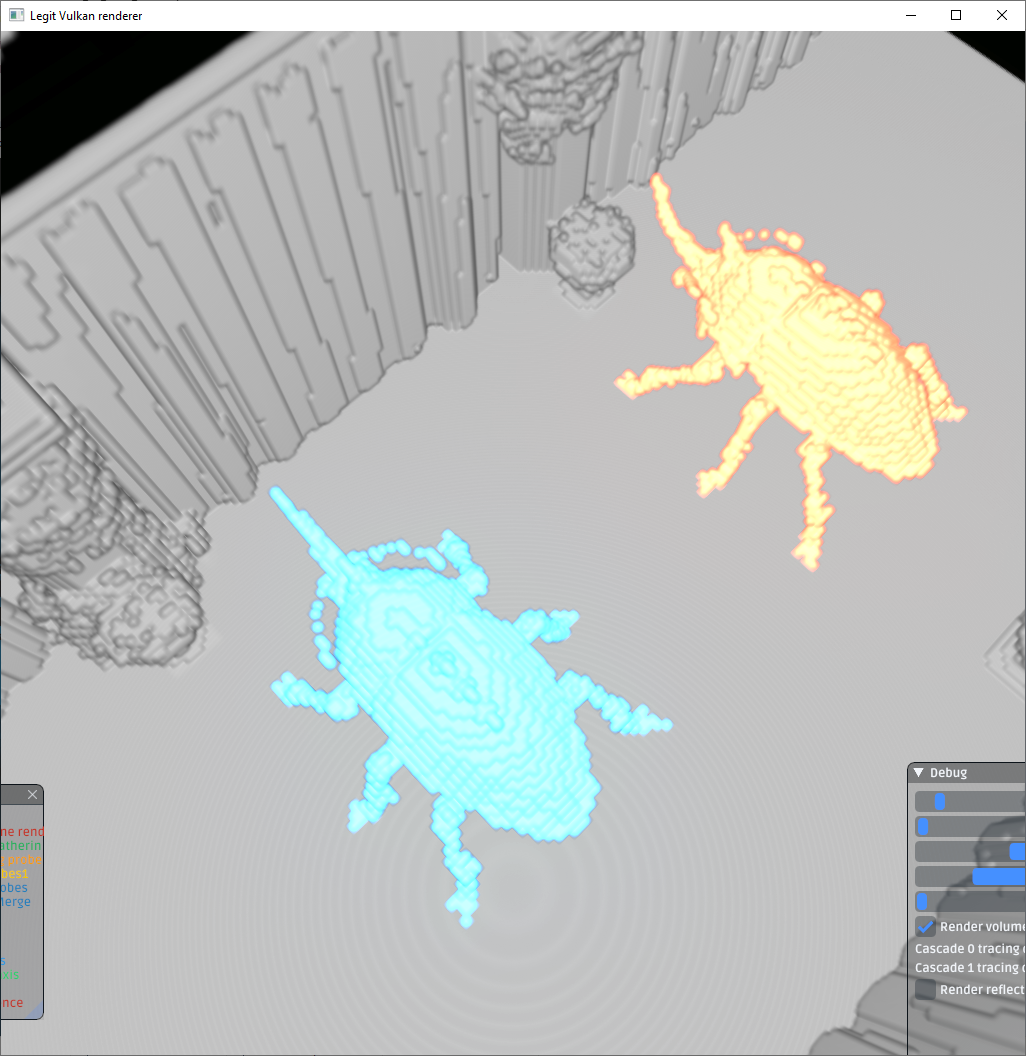
\includegraphics[width=0.3\columnwidth]{images/radiance_3d_voxels.png}
  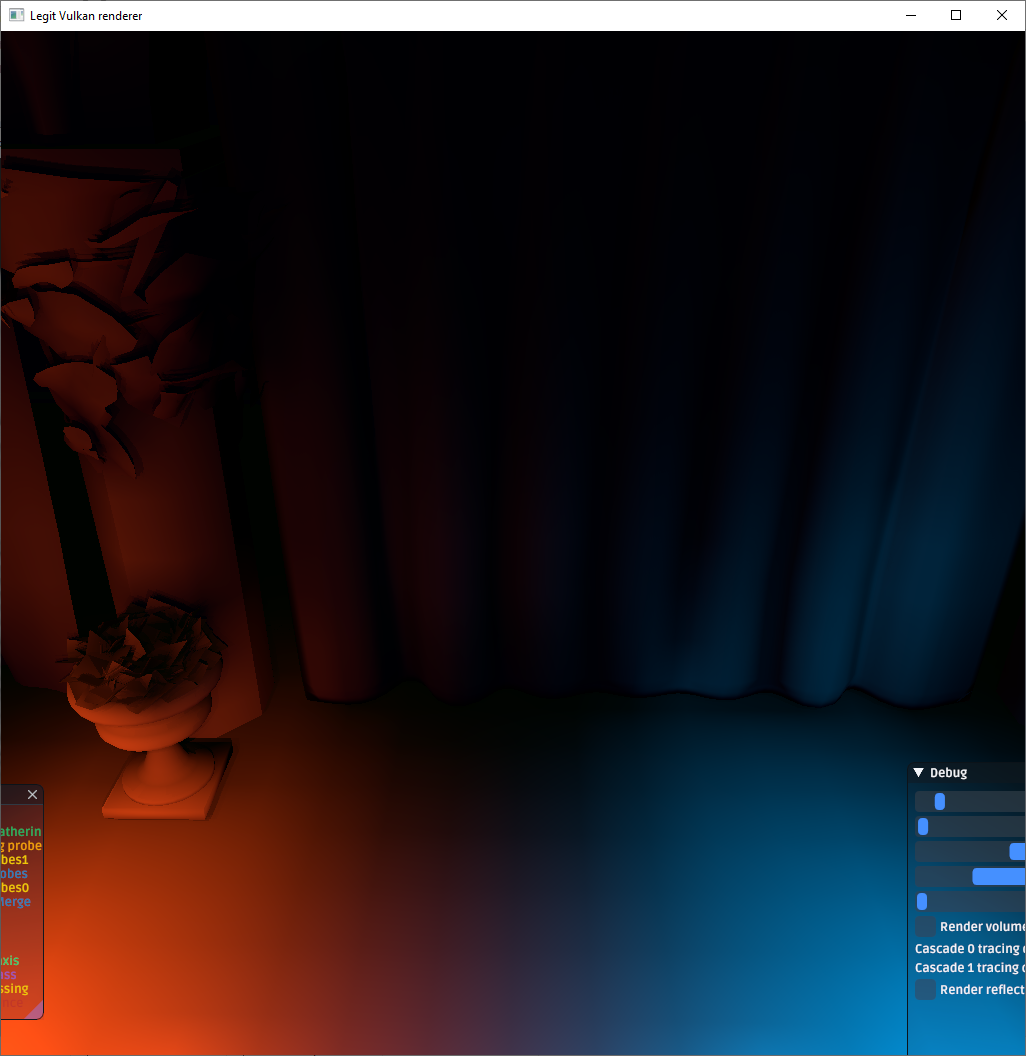
\includegraphics[width=0.3\columnwidth]{images/radiance_3d_from_offscreen.png}
  \caption{\label{fig:radiance_3d_offscreen}
     Left: voxelized representation of the scene. Right: demonstration of indirect light coming from offscreen, which is possible since this technique works in worldspace rather than screenspace.}
\end{figure}

The advantage of storing world space radiance cascades instead of screenspace cascades is that world space cascades allow querying for radiance values anywhere in the world, when the screenspace version only allows one to query radiance on the surface of gbuffer. In practice this means that techniques such as atmospheric scattering or rendering participating medium are only possible with a 3d grid of probes.

Even though the entire hierarchy of 3d cascades takes only as much memory as its cascade 0, it can be still prohibitively expensive, because storing a 3d grid associated with just cascade 0 comes with a very high cost, its their storage requirements scale as the size of the scene cubed, which is often beyond what is acceptable.

However, for a full 3d grid of probes it is possible to employ radiance interval extension \ref{eq:extending_intervals} that allows for a dramatic time reduction on raymarching the scene by replacing a linear-time raymarcher with a short-range raymarching + a couple of iterations of exponential extension. In practice this results in 3d grids being acceptable in terms of computation time, but quite expensive in terms of storage. That being said, a hierarchy of 3d radiance cascades should be basically a drop-in improvement for any implementation that uses a uniform grid of radiance probes.

\clearpage
\subsection{Direct radiance field renderer}
\label{sec:direct_radiance_field}
In order to explore properties of radiance cascades, I implemented a separate program that renders their stored radiance fields directly. More specifically, first a radiance field of a volume is precalculated by path tracing during precomputation and is then stored into a surface radiance cascade hierarchy of a single quad. Then, in runtime this quad is rendered and shaded with radiance retrieved from this radiance cascade hierarchy. This setup effectively allows observing the initial volume and to render it with fully precomputed radiance (including specular lighting, multiple light bounces and refraction) in less than 0.5ms on GTX3060 (see Figure \ref{fig:cascade direct rendering}). The exact encoding scheme used in this case is identical to the one discussed in Section \ref{sub:surface_scaling}.

\begin{figure}[htb]
  \centering
  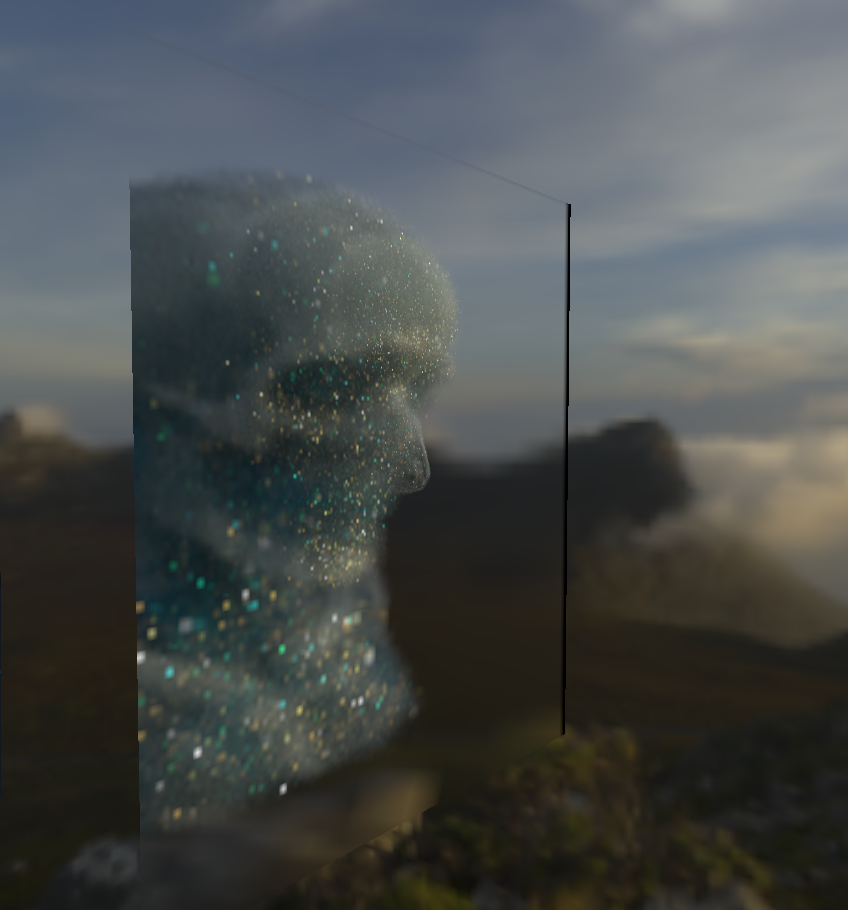
\includegraphics[width=0.32\columnwidth]{images/cropped_left_2.png}
  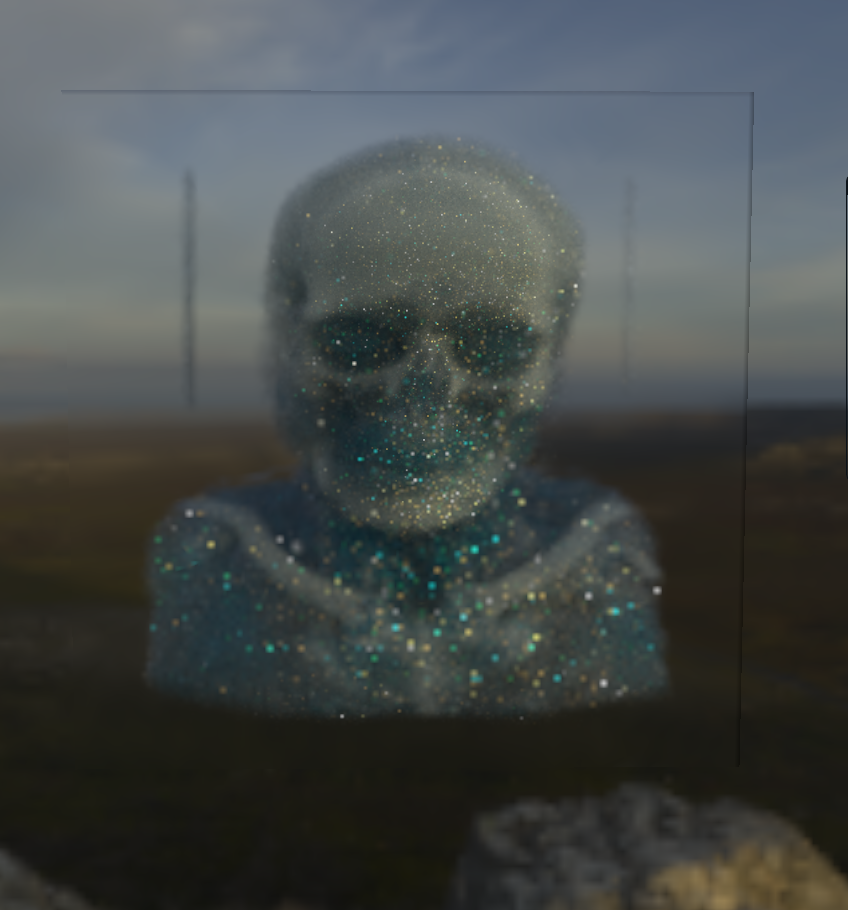
\includegraphics[width=0.32\columnwidth]{images/cropped_center_2.png}
  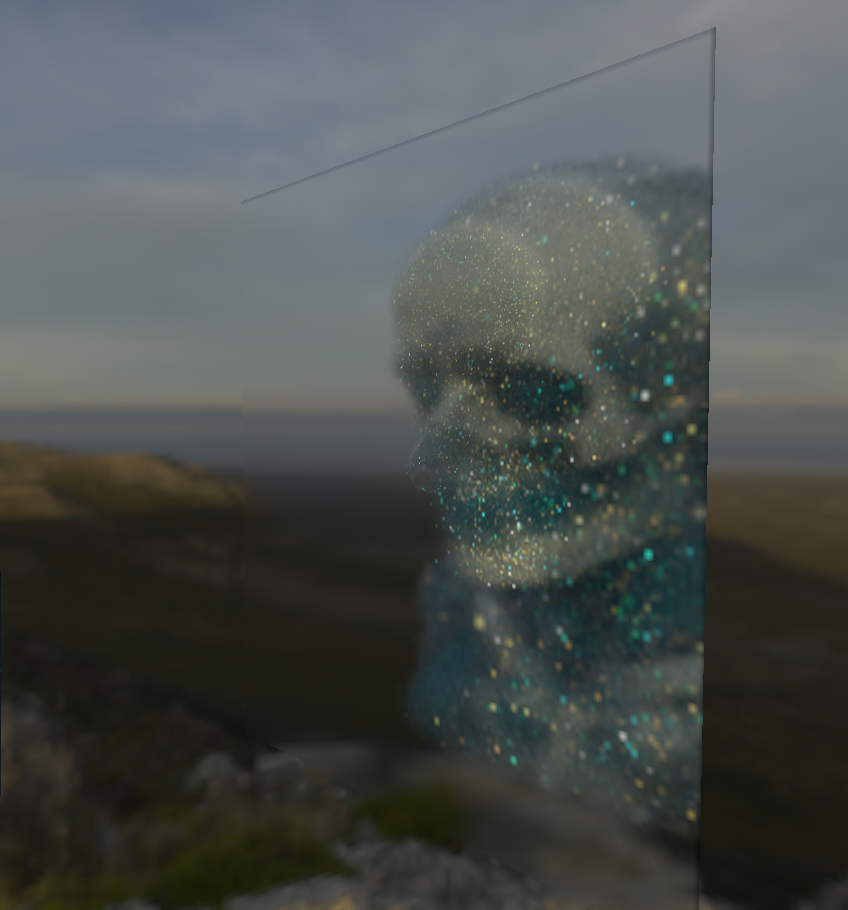
\includegraphics[width=0.32\columnwidth]{images/cropped_right_2.png}
  \caption{\label{fig:cascade direct rendering}
     A demo for directly observing radiance field encoded in \emph{radiance cascades}. Precomputed path traced volumetric data is stored in surface radiance cascades of on a quad, allowing to render it from an arbitrary view point in 0.5ms on GTX3060.}
\end{figure}

\clearpage
\subsection{Screen space probes with world space radiance intervals}
It's also possible to calculate one world-space bounce of indirect by using screenspace radiance cascade. In order to achieve this, a hierarchy of image-space probes akin to \emph{surface radiance cascades} \cref{sec:direct_radiance_field} can be used, where probes of cascade $i$ are represented as octahedral maps of size $\sim 2^i \cdot 2^i$ texels each and probes are placed on the depth buffer $~2^i$ pixels apart. This probe arrangement is very similar to \cref{fig:surface_cascades} and the only difference is that instead of being placed on a flat surface, probes are placed on the depth buffer geometry.

In order to interpolate radiance interval inside one such a cascade, bilateral interpolation is used in space (so that only adjacent probes with similar depth contribute) and bilinear interpolation is used in direction.

This arrangement scales differently to a flatland-like implementation used in PoE2, it also works much less efficiently than screenspace raymarching, but its main advantage is that probes of size $\sim 2^i \cdot 2^i$ can capture radiance intervals in world space, allowing invisible sources of indirect light to illuminate geometry on the screen. This include off-screen emissive or directly lit surfaces as well as surfaces occluded in the depth buffer. In comparison, PoE2 implementation uses probes that scale as $\sim 2^i \cdot 1$ (same as flatland), can't capture offscreen light sources, but it works 1 to 2 orders of magnitude faster in the end due to dramatically more efficient optimizations possible due to screenspace raymarching.

To query radiance intervals between probes, bilateral interpolation is used, which reduces influence of adjacent probes that have a different value of the depth buffer associated with them. For directional interpolation, a simple bilinear interpolation is used.

World space radiance intervals can be calculated in many different ways, including volume raymarching, raytracing (software and hardware): any acceleration structure can work, as long as it allows querying ray segments. The implementation that this work uses signed distance field  \footnote{Authors of these SDFs (in the order of occurrence) are:  WAHa\_06x36, iq, leon, Kali, jb} raymarching purely because of convenience.

This implementation also utilizes reprojection: each cascade can be efficiently reprojected from the previous frame to allow temporal accumulation over time. This allows to dramatically increase long-term convergence by sacrificing some lighting responsiveness.

\begin{figure}[htb]
  \centering
  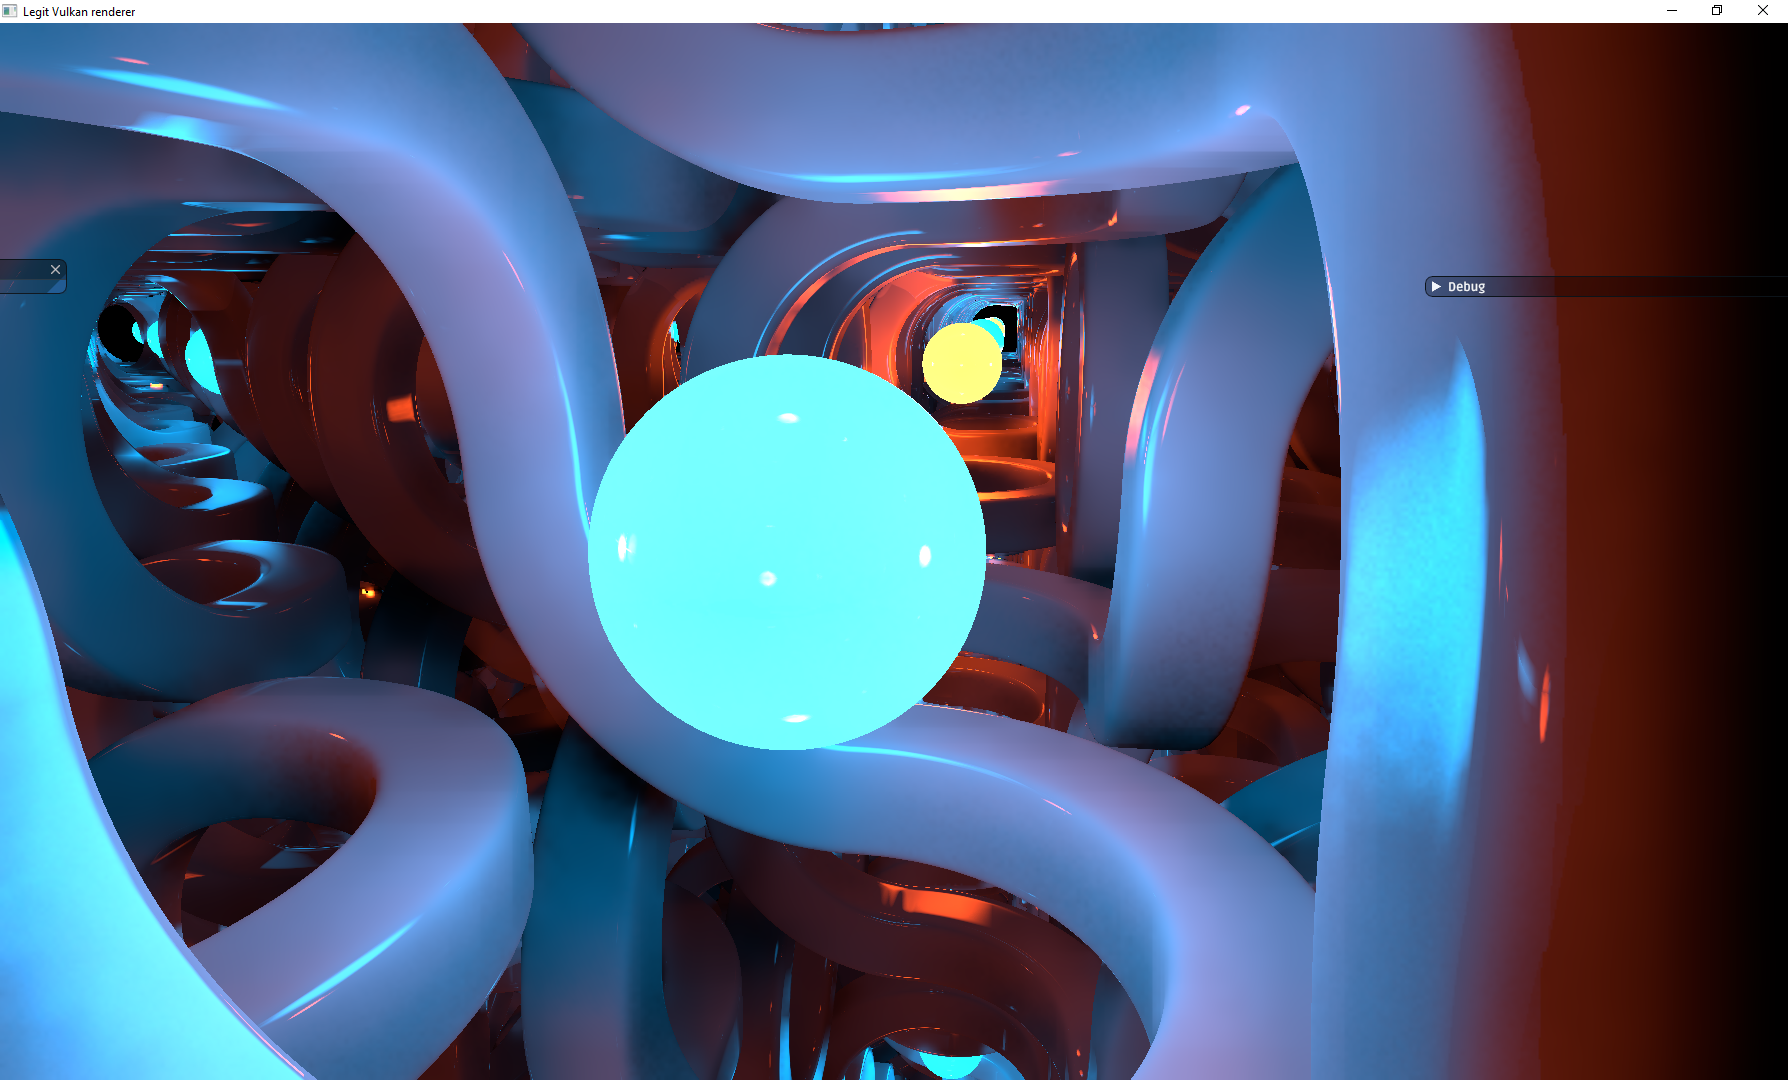
\includegraphics[width=0.49\columnwidth]{images/sdf_reprojection_truchet.png}
  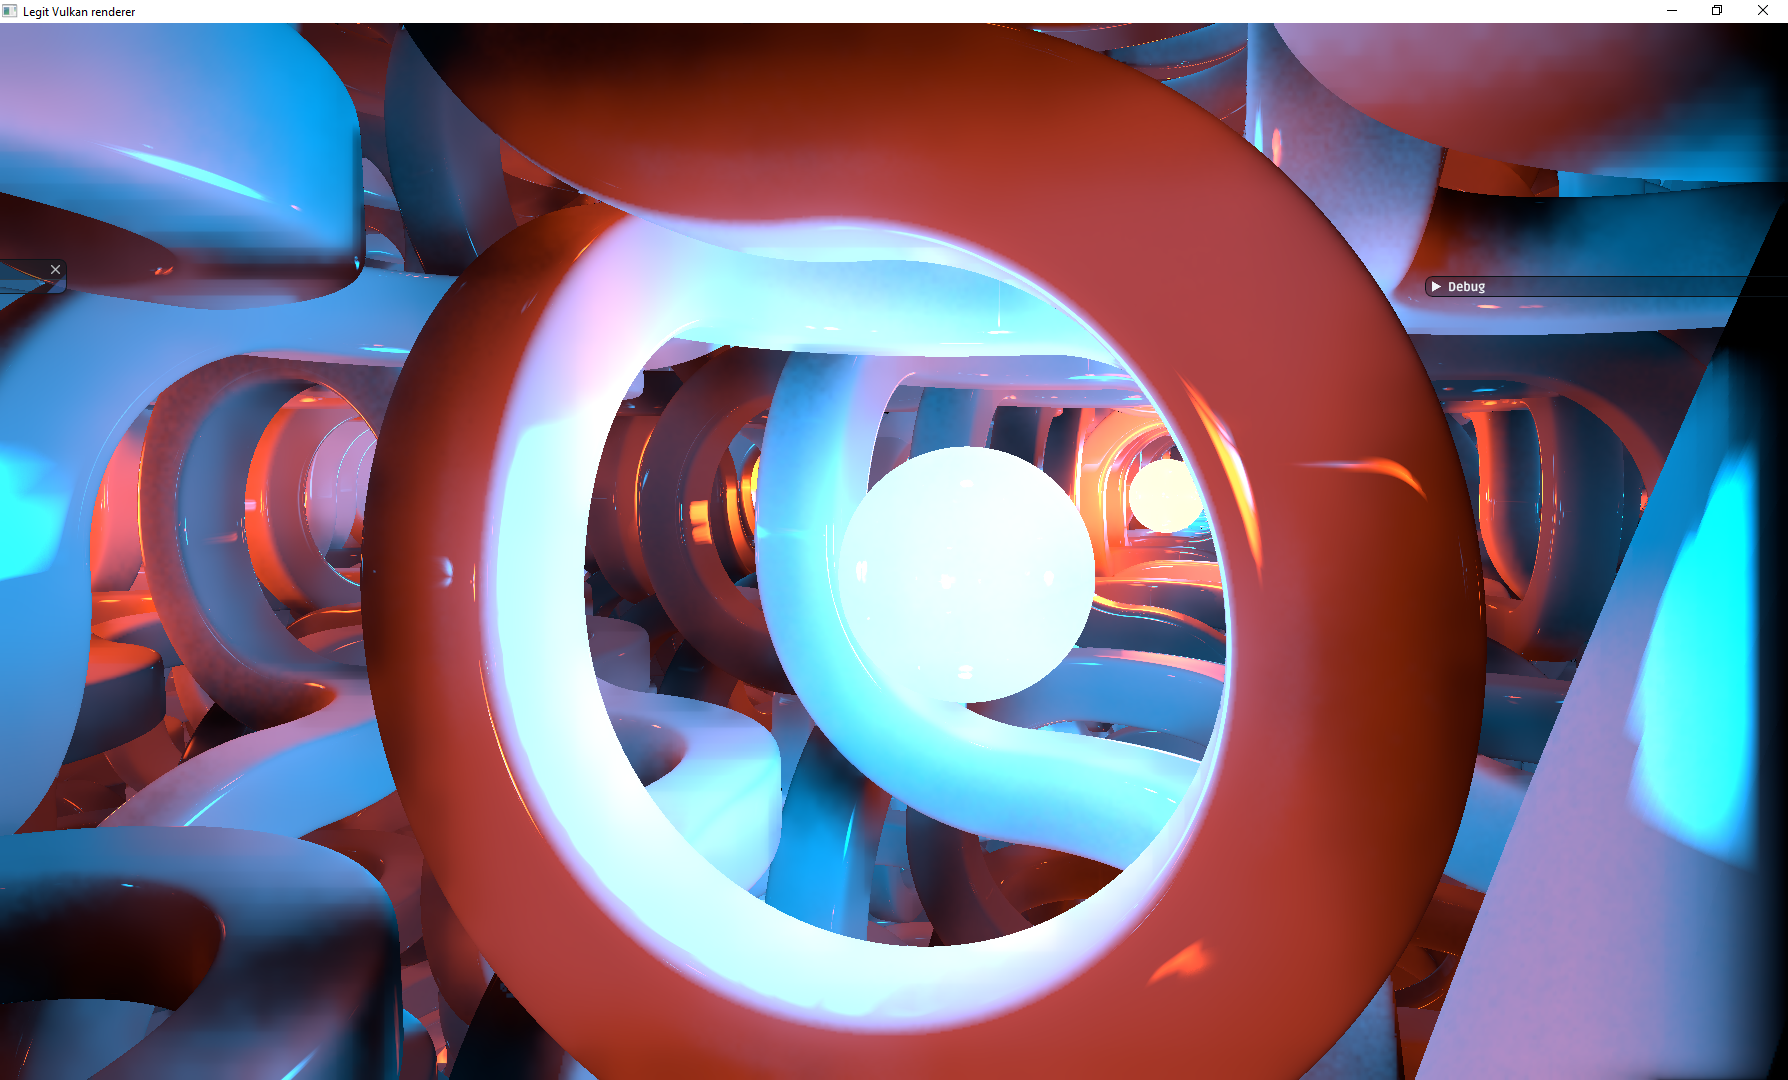
\includegraphics[width=0.49\columnwidth]{images/sdf_reprojection_truchet2.png}
  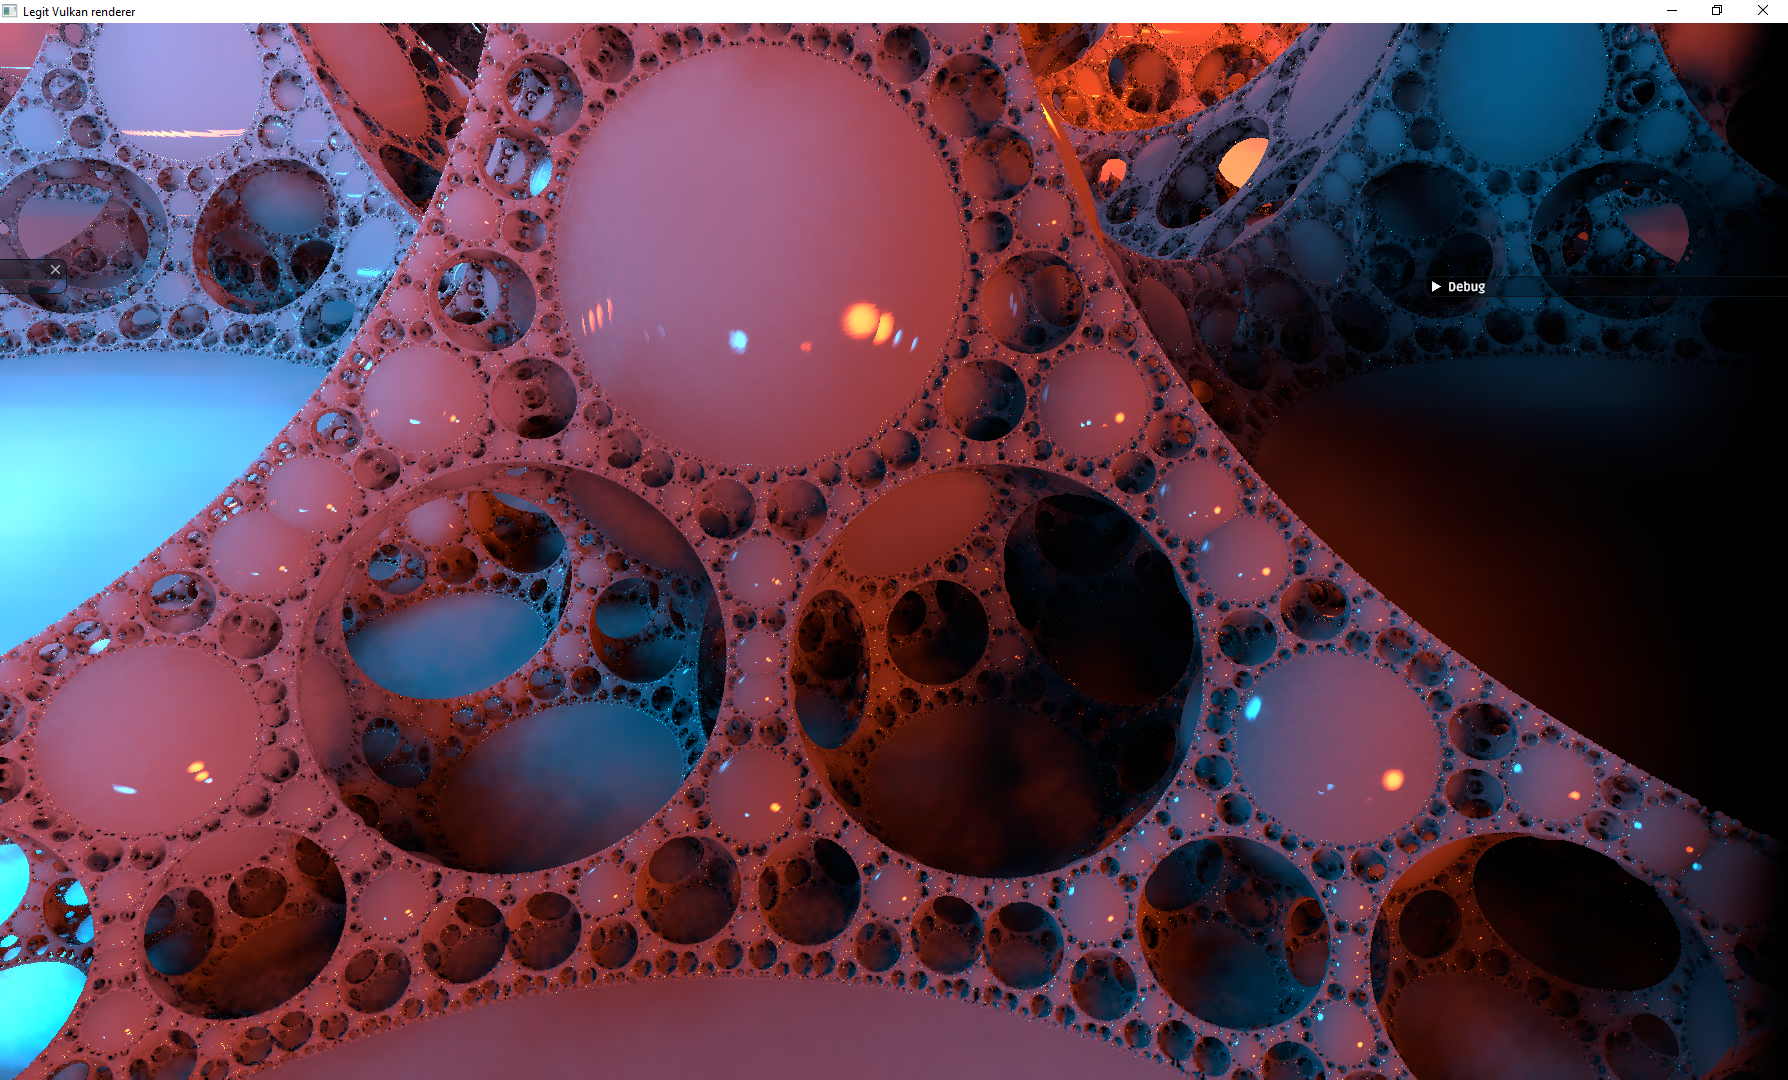
\includegraphics[width=0.49\columnwidth]{images/sdf_apollonian.png}
  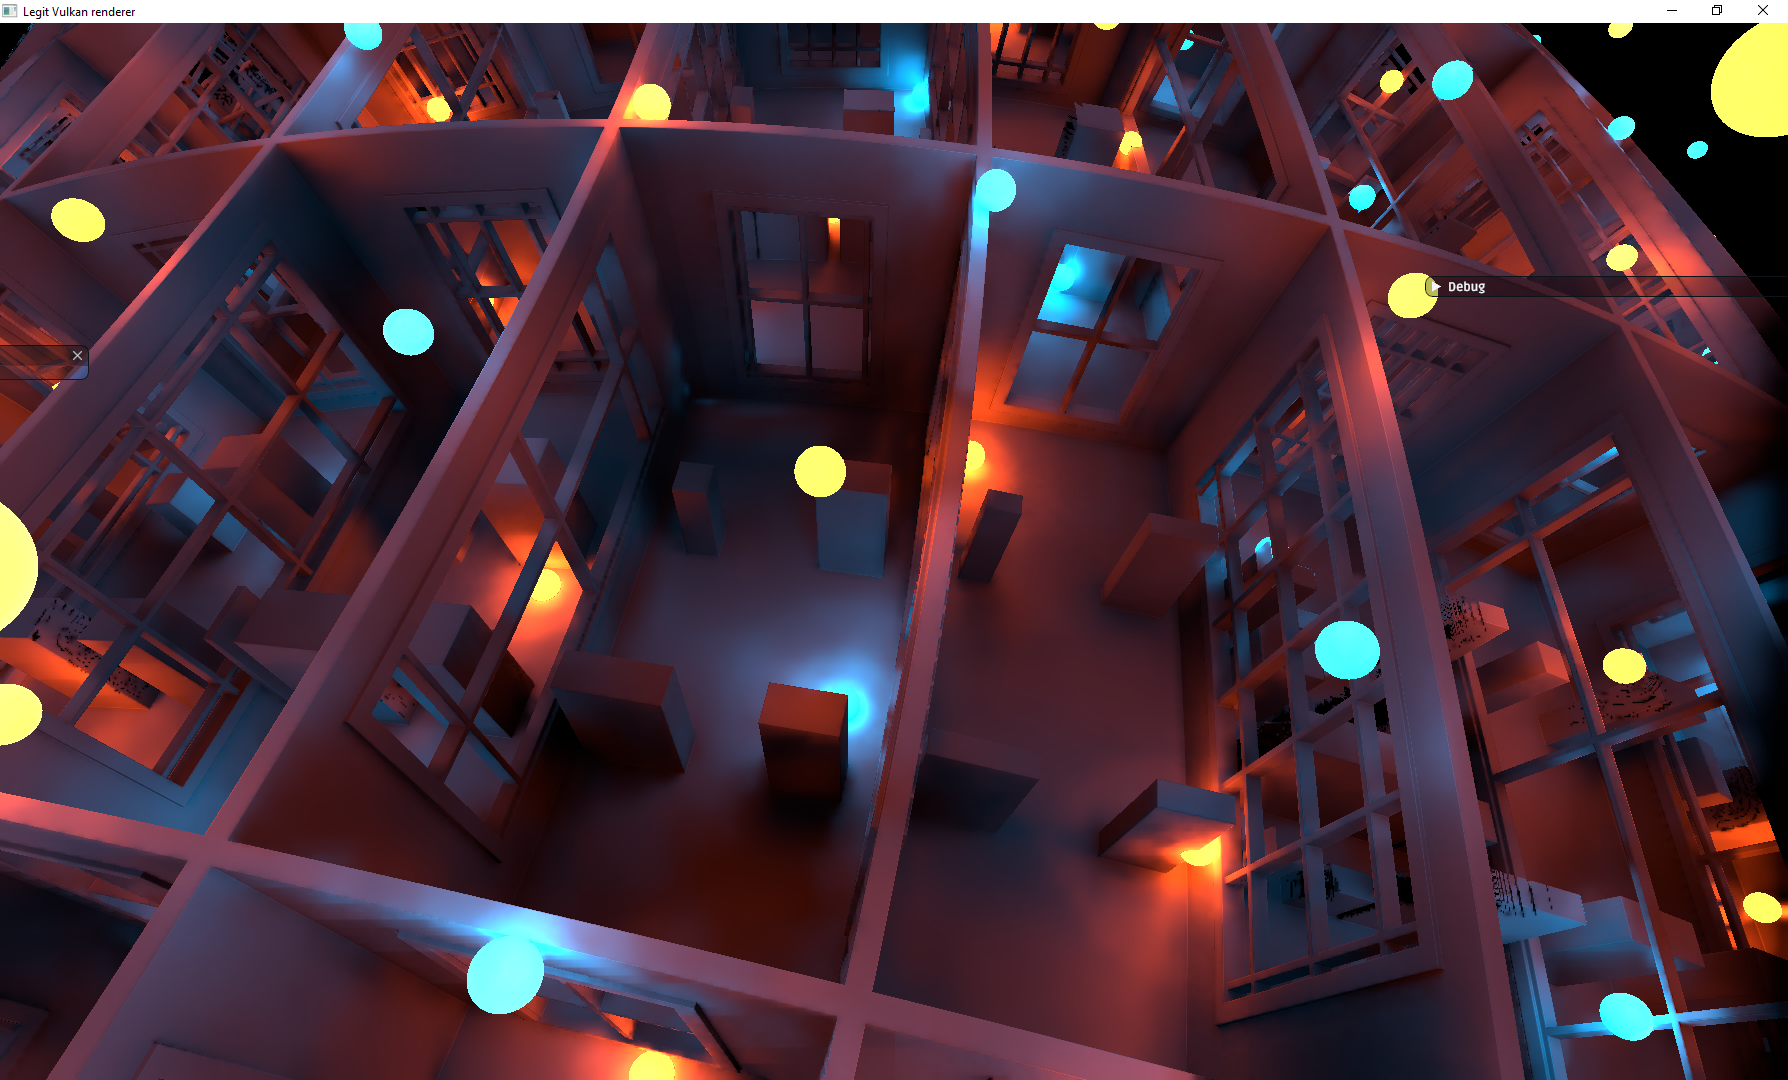
\includegraphics[width=0.49\columnwidth]{images/sdf_leon_torus_1.png}
  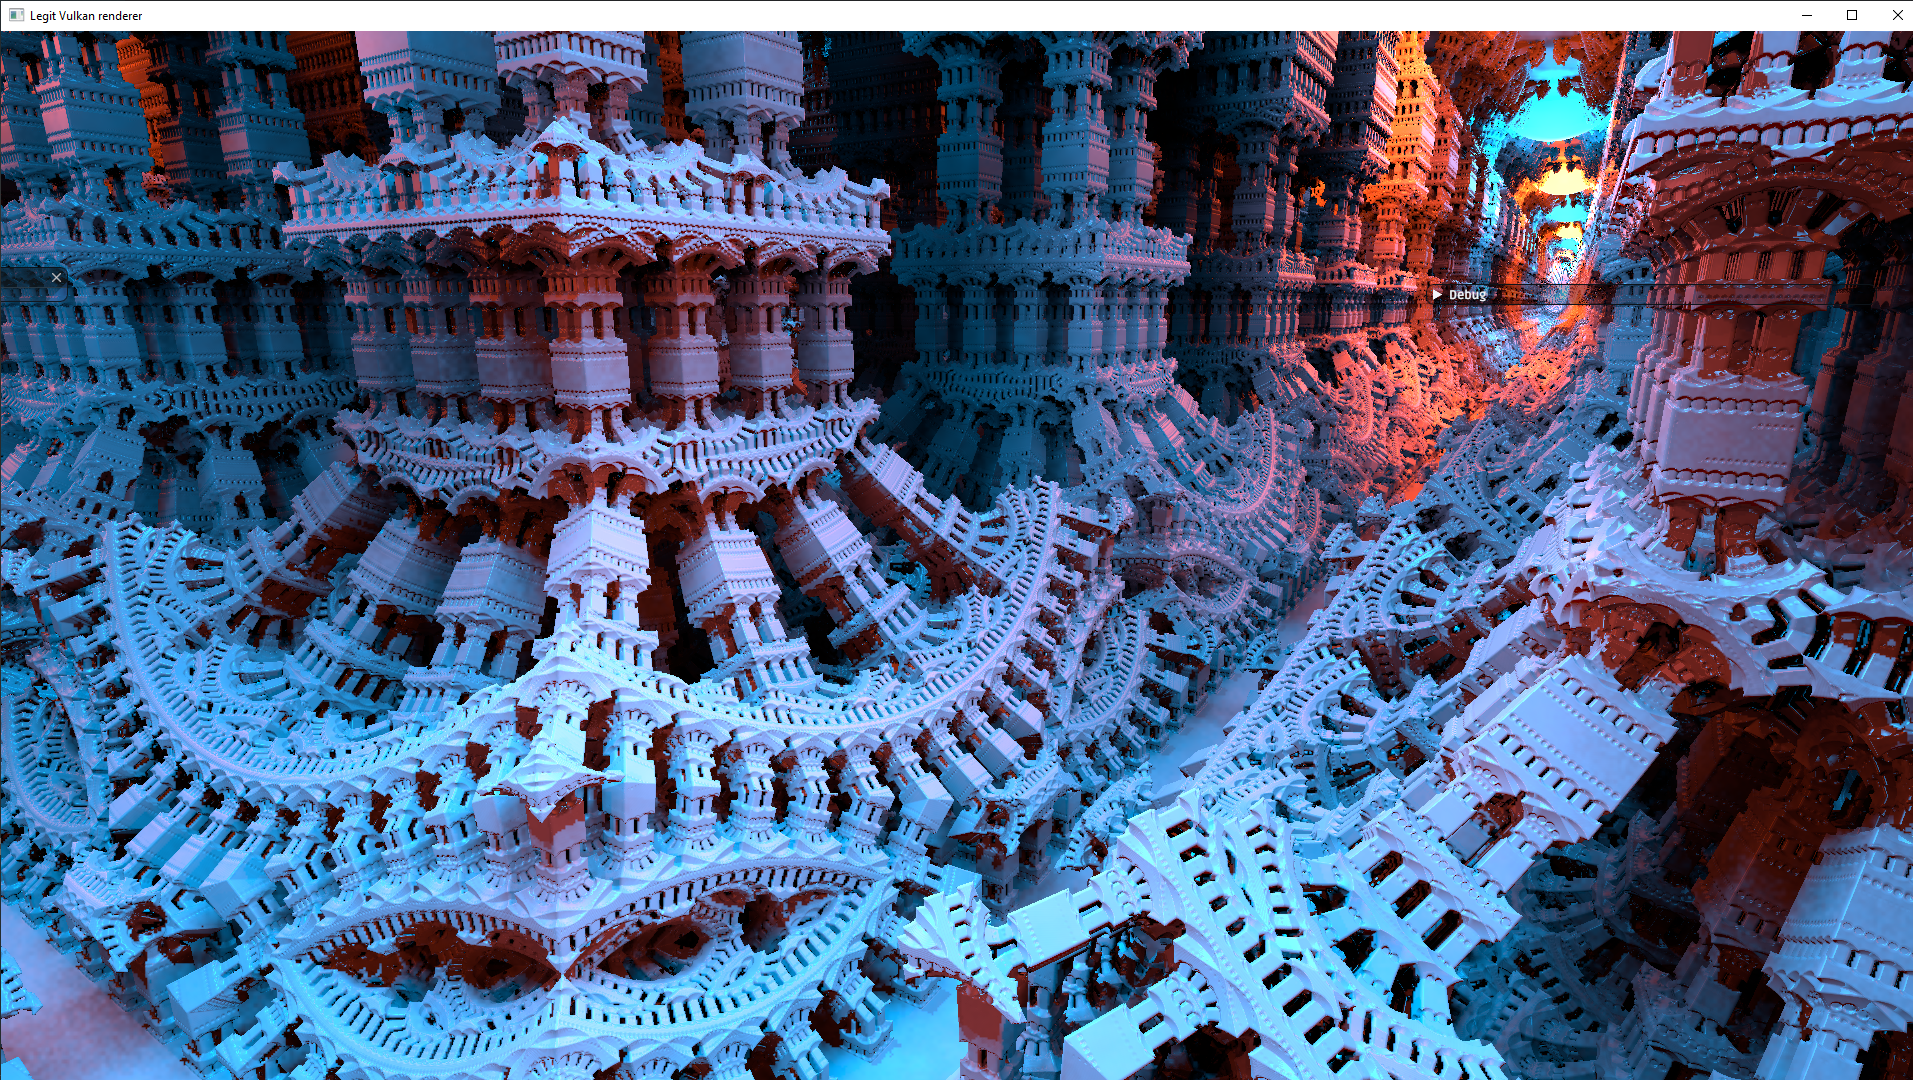
\includegraphics[width=0.49\columnwidth]{images/sdf_temple.png}
  \includegraphics[width=0.49\columnwidth]{images/sdf_fractal_1.png}
  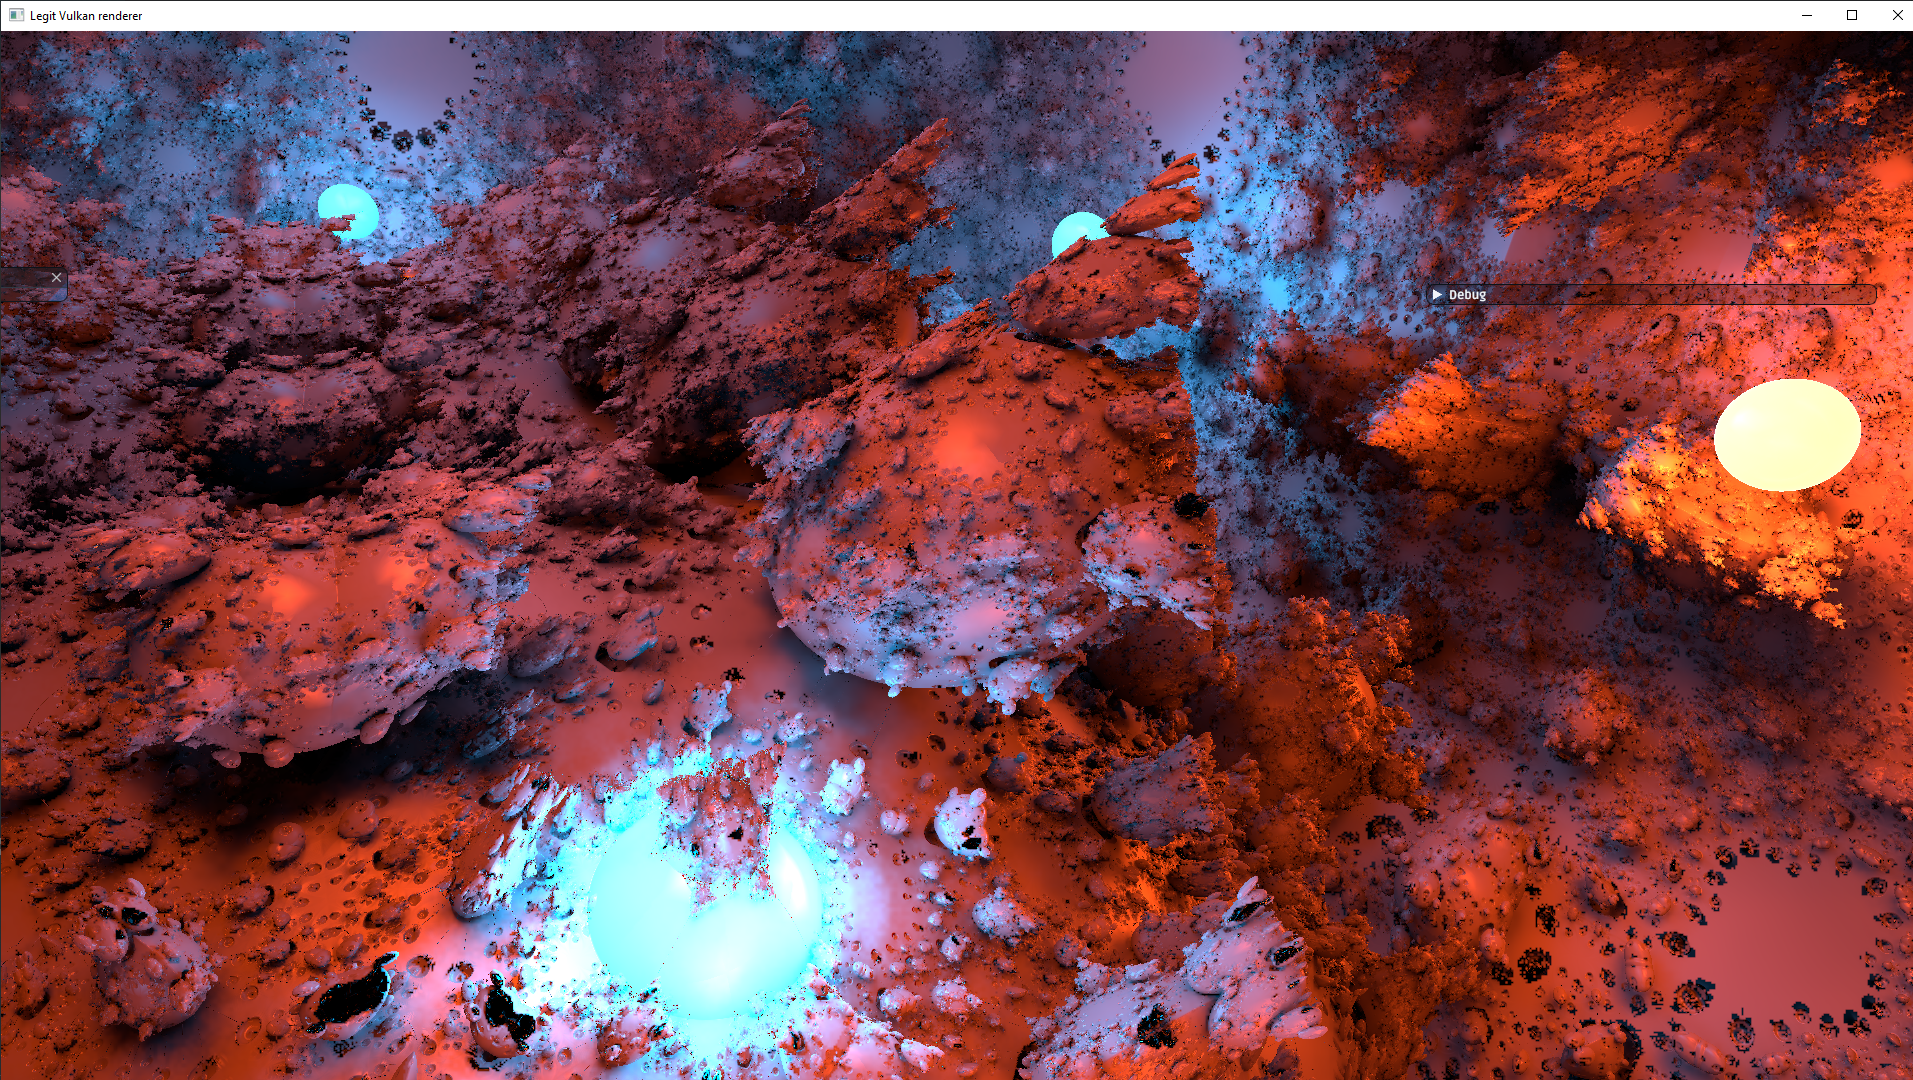
\includegraphics[width=0.49\columnwidth]{images/sdf_fractal_2.png}
  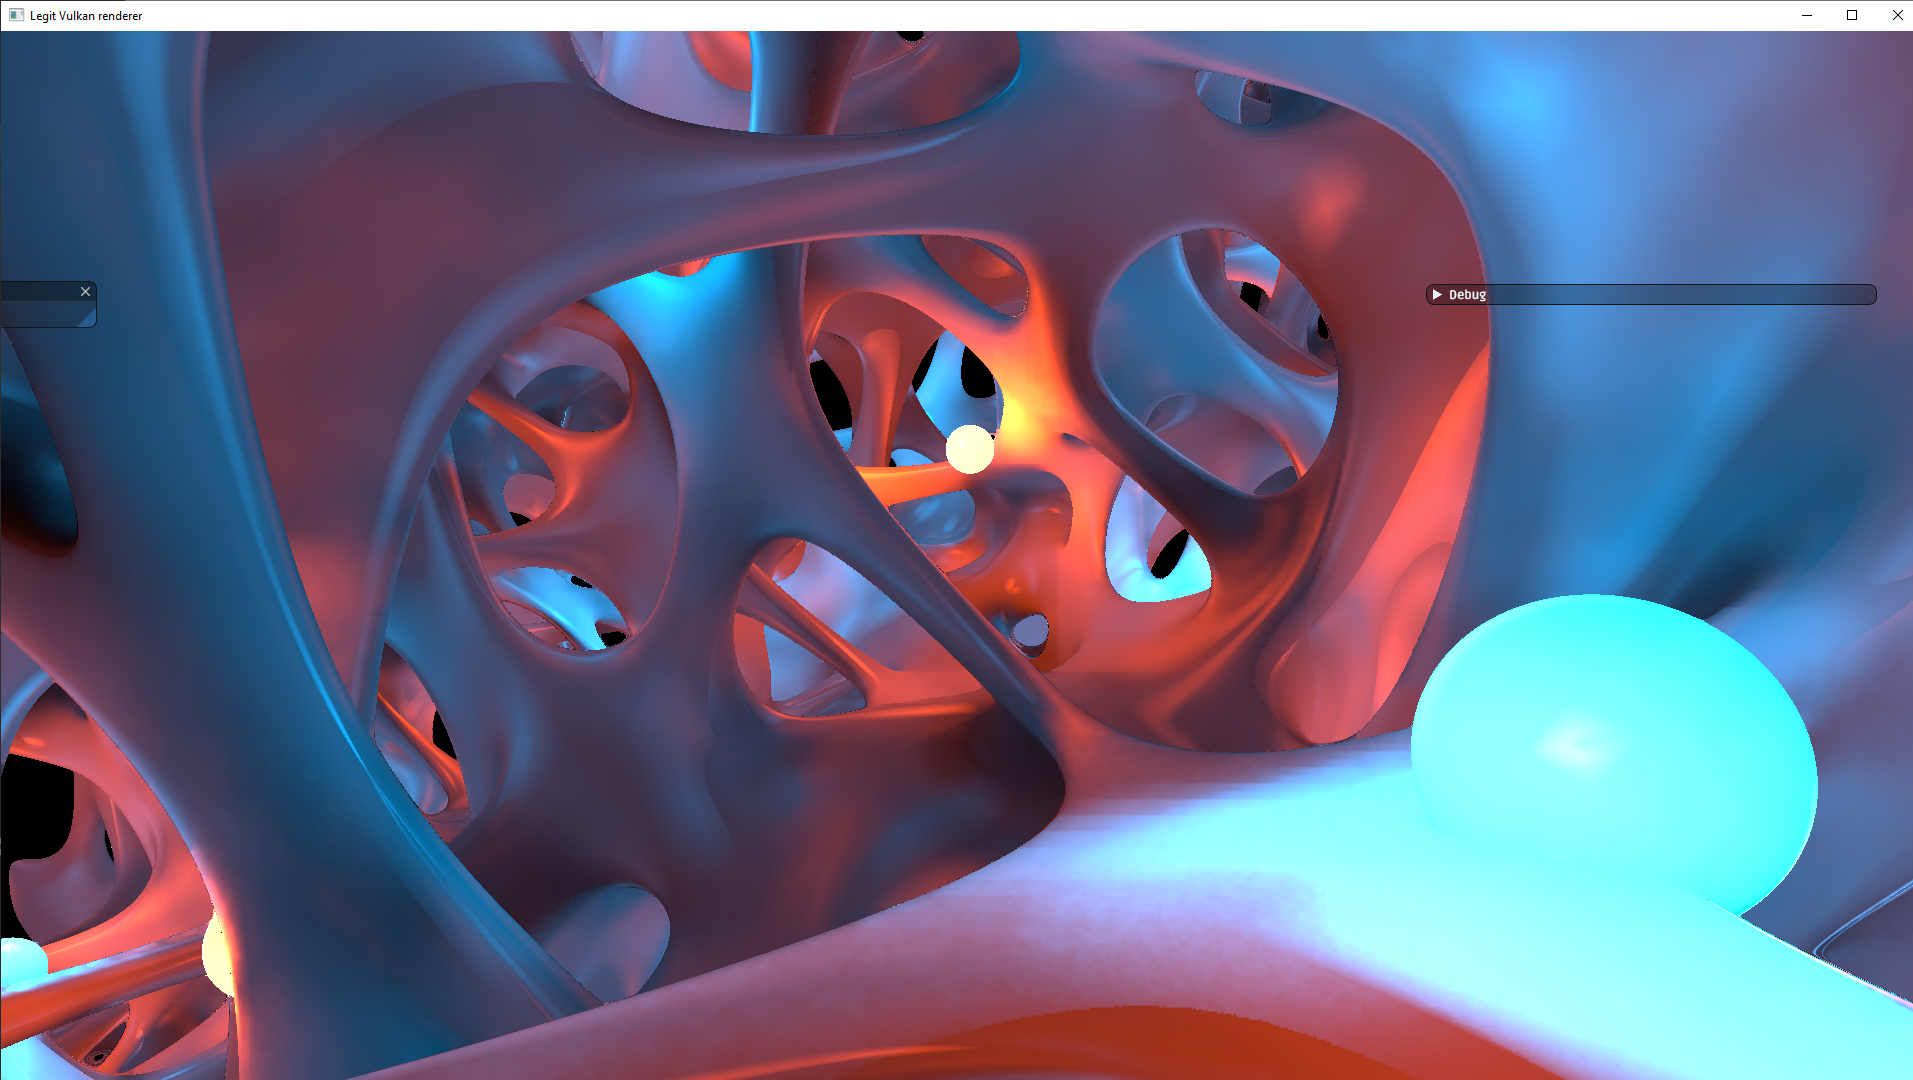
\includegraphics[width=0.49\columnwidth]{images/sdf_goopy2.png}
  \caption{\label{fig:sdf_world_space}
     A demo of world space radiance intervals encoded in screenspace probes. Images demonstrate the possibility of capturing off-screen world-space lighting and occlusion information in screenspace probes. Each scene is represented as an analytical SDF and it's used for world space raymarching while calculating radiance cascades. Each frame takes about 30-50ms to calculate on GTX3060 and each novel view takes 0.1-0.5s to converge due to temporal accumulation(exact time depends on fractal used).}
\end{figure}

\begin{figure}[htb]
  \centering
  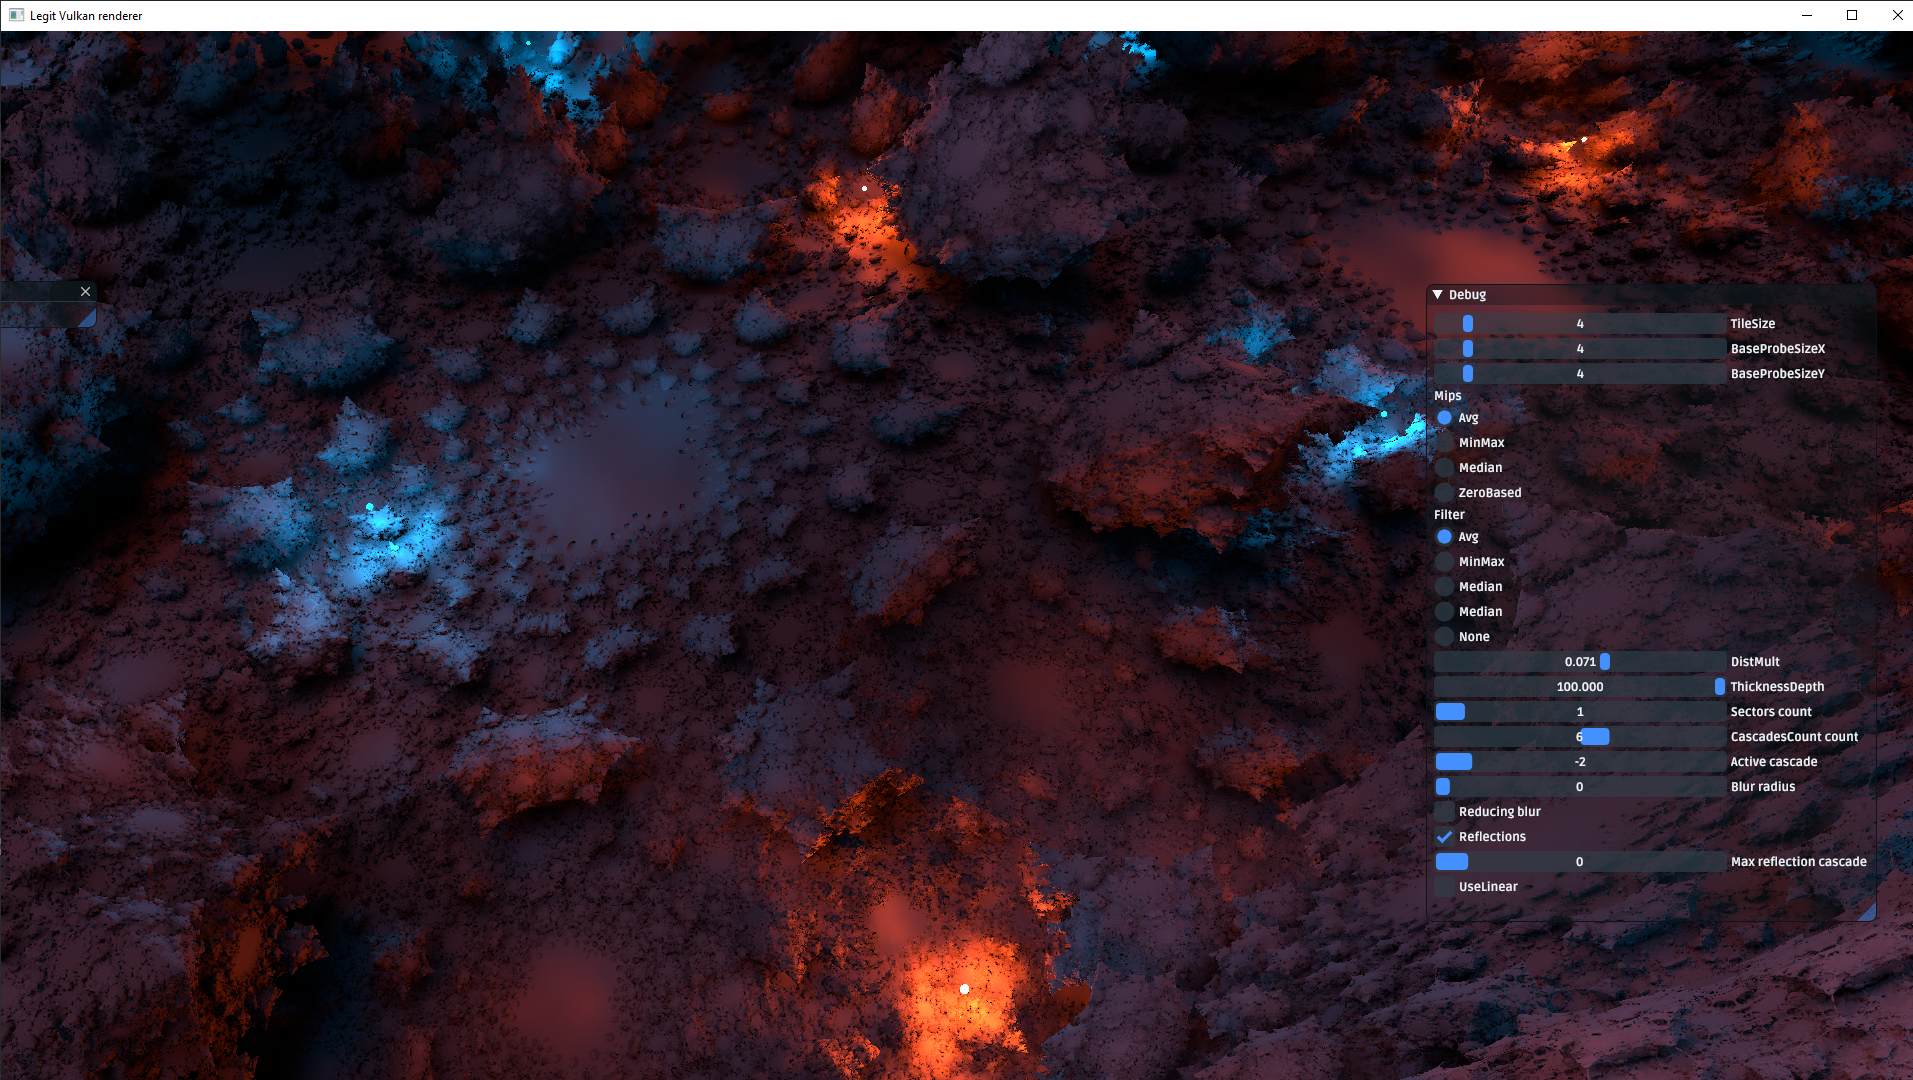
\includegraphics[width=\columnwidth]{images/sdf_stress_tiny.png}
  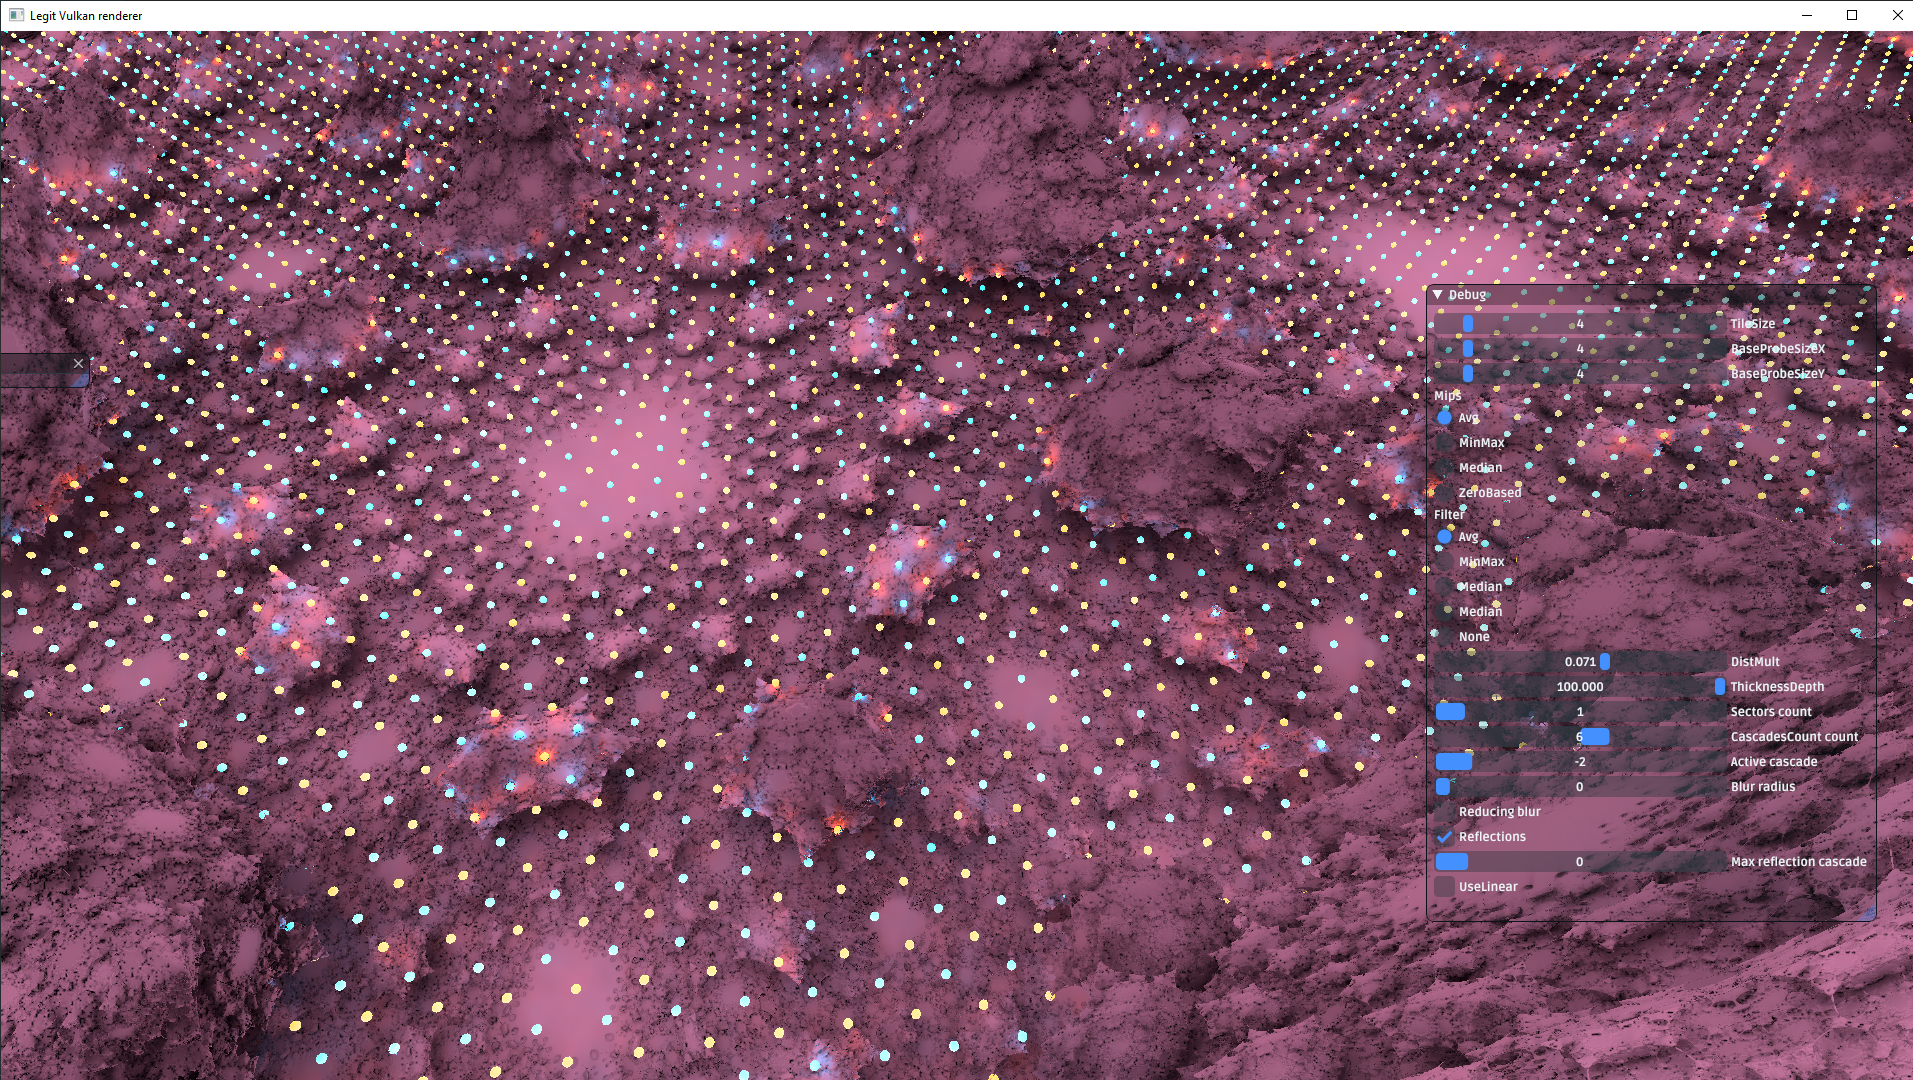
\includegraphics[width=\columnwidth]{images/sdf_stress_many.png}
  \caption{\label{fig:sdf_stress_test}
     Top: stress test with small indirect light sources, Bottom: stress test with many light sources. Indirect light even from small emissive surfaces can be observed and performance of the method does not depend on their number.}
\end{figure}
\clearpage
\section{Limitations}
Radiance cascades do have their limitations, however. Most importantly, even though radiance cascades scale very well asymptotically, the constant part of their complexity can be quite high. For example, even though storing the "tail" of a full 3d radiance field takes only as much space as storing its cascade 0, just storing a cascade 0 is practically equivalent to voxelizing the entire scene -- this is often a "dealbreaker" for large-scale scenes.

Even in image space, even though all cascades add up to have the same cost as cascade 0, calculating just cascade 0 in a high level of detail can take milliseconds, which can already be over the budget for some realtime applications.

Another limitation of this work is that for the sake of simplicity it only provides an asymptotic scaling analysis, completely omitting considerations behind choosing any actual initial values. Values such as cascade 0 linear stepping $\Delta_p$, angular stepping $\Delta_\omega$, its corresponding radiance interval, etc -- these arbitrary parameters dramatically affect both accuracy and performance of the method, and can take some amount of fiddling to get right.

At the time of writing this article, the most successful practical implementation of this method (used in Path of Exile 2) uses exclusively screenspace data to raymarch radiance intervals. While this is highly efficient and is arguably quite convenient for PoE2, it has obvious screenspace limitations: light sources outside of the view don't cast indirect light, invisible occluders don't cast shadows and there's no data about any geometry behind the depth buffer. It is important to mention that these limitations stem from the fact that cascades are built by raymarching screenspace data, and \textbf{not} due to the fact that cascades themselves are stored in screenspace. In fact, screenspace radiance cascades can store world space radiance intervals and this would eliminate any screenspace-related artifacts. However, it is unclear how to calculate world space radiance intervals anywhere near as efficiently as by raymarching in screenspace. While it is possible to do so with hardware raytracing, and while such an approach would indeed scale asymptotically just as well, the constant cost would be an order of magnitude higher compared to raymarching in screenspace.


\section{Conclusions and further work}
Radiance cascades are a novel data structure with unusually effective scaling parameters where rays get exponentially cheaper with every new cascade, which is possible because instead of casting rays explicitly, radiance cascades instead store radiance intervals that can be combined into rays when needed, which has proven to be much more efficient. Such approach relies on a fundamental assumption about inherent structure of radiance fields, \emph{the penumbra hypothesis} that ties together spatial and angular discretization frequency of typical radiance fields intervals that allows discretizing them very efficiently. While it might be possible to construct synthetic cases for which this hypothesis breaks, in practice it seems to hold most of the time.

As a consequence, using radiance cascades practically removes one of the most fundamental limitations of global illumination methods: the total number of rays available. This is distinctly different from methods that calculate rays explicitly (instead of using radiance intervals), as their calculation time as well as memory required for storage scales linearly with total number of rays.

A very important property of every approximate rendering algorithm is how its quality degrades with less samples/precision. And radiance cascades degrade in a very interesting way where normally sharp shadows become blurrier as if they were cast by an area light source, which looks quite natural in practice. Achieving penumbras by design is a very important property and is distinctly different from most other shadowing algorithms that rely on building sharp shadows first and then wasting resources on blurring them. 

Radiance cascades are primarily useful for solving diffuse global illumination, but since they provide a general purpose way of encoding radiance, they can also be used with arbitrary BRDF's (including specular) and can even be used for direct observation for purposes such as rendering precomputed path traced data.

While this work primarily utilizes very efficient screenspace raymarching to calculate radiance intervals, it has its obvious limitations, and it would be interesting to explore other ways such as utilizing raytracing or some other sort of a worldspace approach.


\begin{enumerate}
\item ``The Rendering Equation \cite{Immel:1986:RMN:15886.15901,Kajiya:1986:RE:15922.15902} relates the incoming and outgoing light at a surface...''
\item ``Immel et al.'s paper~\shortcite{Immel:1986:RMN:15886.15901} uses a directional parameterization...''
\end{enumerate}

\small
\bibliographystyle{jcgt}
\bibliography{RadianceCascades}

\section*{Index of Supplemental Materials}
When supplemental materials such as video, data sets, and source code are provided with an article, briefly describe them by directory or filename here.

\section*{Author Contact Information}

\hspace{-2mm}\begin{tabular}{p{0.5\textwidth}p{0.5\textwidth}}
Alexander Sannikov \newline
Grinding Gear Games \newline
6 Alderman Dr \newline
Henderson, Auckland, New Zealand 0612 \newline
\href{mailto:donxenapo@gmail.com}{donxenapo@gmail.com} \newline
\href{https://www.youtube.com/@Alexander_Sannikov}{https://www.youtube.com/@Alexander\_Sannikov} \newline
\href{https://www.linkedin.com/in/alexander-sannikov-9964aa188/}{https://www.linkedin.com/in/alexander-sannikov-9964aa188/}

\end{tabular}


\afterdoc

\end{document}
